\documentclass[12pt,american]{report}
\usepackage{times}
\usepackage[T1]{fontenc}
\usepackage[utf8]{inputenc}
\usepackage{graphicx}
\usepackage{geometry}
\usepackage{siunitx}
\usepackage{pgfplots}
\usepackage{hyperref}
\usepackage{longtable}
\usepackage{caption}
\usepackage{url}
\usepackage{grffile}
\usepackage{ulem}
\usepackage{booktabs}
\usepackage{fancyvrb}
\usepackage{amssymb}
\usepackage{amsmath}
\usepackage{ifxetex}
\usepackage{ifluatex}
\geometry{verbose,letterpaper,tmargin=1in,bmargin=1in,lmargin=1.5in,rmargin=1in} %% sets paper size and margins
\usepackage{setspace}
\usepackage[square]{natbib}
\bibliographystyle{unsrtnat}
\usepackage{texments}
% \usepackage{amssymb}
\usepackage[]{algorithm2e}
\usestyle{xcode}


%\singlespacing        %% 1-spacing (default)
%\onehalfspacing       %% 1,5-spacing
%\doublespacing        %% 2-spacing

\pagestyle{plain}      %% select plain page style: no headers, page numbers center bottom

%% uncomment the following to include headers (e.g., to keep track of draft versions). Also change pagestyle to fancyplain:
%\rhead[\fancyplain{}{\leftmark}]%0
%      {\fancyplain{}{Draft 04/08 -- \thepage}}
%\cfoot[\fancyplain{Draft 04/08 -- \thepage}{}]{\fancyplain{Draft 04/08 -- \thepage}{}}

\begin{document}

\pagenumbering{roman}        %% roman page numbers for front matter

\renewcommand\thepage{}
% \pagestyle{plain}
\begin{center}
\textbf{FOLDLINGS: Interactive Pop-Up Card Design}
\vspace{0.4cm}

A Thesis\\ [0.4cm]
Submitted to the Faculty \\ [0.4cm]
in partial fulfillment of the requirements for the \\[0.4cm]
degree of \\[0.4cm]
Master of Science\\in\\Computer Science with a Concentration in Digital Arts\\[0.4cm]
by\\[0.5cm]
Nook Harquail\\[0.4cm]
in Conjunction with Marissa Allen \\[0.5cm]
Department of Computer Science \\ [0.4cm]
DARTMOUTH COLLEGE \\ [0.4cm]
Hanover, New Hampshire \\[0.4cm]
September 1, 2015 % that you will submit your signed thesis
\vspace{1.5cm}

\end{center}

Examining Committee:

\begin{flushright}
Advisor \line(180, 0){110} \\
Emily Whiting \\[1cm]

Member \line(180, 0){110} \\
Lorie Loeb \\[1cm]

Member \line(180, 0){110} \\
Jodie Mack \\[1cm]

% Member \line(180, 0){110} \\
% MEMBER NAME HERE\\[1cm]

%(ALL signatures must be in Black ink, ALL fonts in black ink)

\end{flushright}

\begin{flushleft}
\line(180, 0){110} \\
F. Jon Kull, Ph.D.\\
Dean of Graduate Studies\\[1cm]
%NOTE: the copies you submit must have the original signatures for PhD, one hard copy, for MS, two copies and a pdf of the thesis is required for both degrees.  No Holes, clips or binding on the copy and should be on Quality paper, preferably, Dartmouth Bond.
\end{flushleft}

% \pagestyle{plain}
\begin{center}
\textbf{FRAMESHIFT: SHIFT YOUR ATTENTION, SHIFT THE STORY}
\vspace{0.4cm}

A Thesis\\ [0.4cm]
Submitted to the Faculty \\ [0.4cm]
in partial fulfillment of the requirements for the \\[0.4cm]
degree of \\[0.4cm]
Master of Science\\in\\Computer Science with a Concentration in Digital Arts\\[0.4cm]
by\\[0.5cm]
Tim Tregubov\\[0.4cm]
in Conjunction with Rukmini Goswami \\[0.5cm]
Department of Computer Science \\ [0.4cm]
DARTMOUTH COLLEGE \\ [0.4cm]
Hanover, New Hampshire \\[0.4cm]
May 15, 2015 % that you will submit your signed thesis
\vspace{1.5cm}

\end{center}

Examining Committee:

\begin{flushright}
Chair \line(180, 0){110} \\
Lorie Loeb\\[1cm]

Member \line(180, 0){110} \\
Michael Cohen \\[1cm]

Member \line(180, 0){110} \\
Michael Casey \\[1cm]

% Member \line(180, 0){110} \\
% MEMBER NAME HERE\\[1cm]

%(ALL signatures must be in Black ink, ALL fonts in black ink)

\end{flushright}

\begin{flushleft}
\line(180, 0){110} \\
F. Jon Kull, Ph.D.\\
Dean of Graduate Studies\\[1cm]
%NOTE: the copies you submit must have the original signatures for PhD, one hard copy, for MS, two copies and a pdf of the thesis is required for both degrees.  No Holes, clips or binding on the copy and should be on Quality paper, preferably, Dartmouth Bond.
\end{flushleft}







% \pagestyle{plain}
\begin{center}
\textbf{FRAMESHIFT: SHIFT YOUR ATTENTION, SHIFT THE STORY}
\vspace{0.4cm}

A Thesis\\ [0.4cm]
Submitted to the Faculty \\ [0.4cm]
in partial fulfillment of the requirements for the \\[0.4cm]
degree of \\[0.4cm]
Master of Science\\in\\Computer Science with a Concentration in Digital Arts\\[0.4cm]
by\\[0.5cm]
Rukmini Goswami\\[0.4cm]
in Conjunction with Tim Tregubov \\[0.5cm]
Department of Computer Science \\ [0.4cm]
DARTMOUTH COLLEGE \\ [0.4cm]
Hanover, New Hampshire \\[0.4cm]
May 15, 2015 % that you will submit your signed thesis
\vspace{1.5cm}

\end{center}

Examining Committee:

\begin{flushright}
Chair \line(180, 0){110} \\
Lorie Loeb\\[1cm]

Member \line(180, 0){110} \\
Michael Cohen \\[1cm]

Member \line(180, 0){110} \\
Michael Casey \\[1cm]

% Member \line(180, 0){110} \\
% MEMBER NAME HERE\\[1cm]

%(ALL signatures must be in Black ink, ALL fonts in black ink)

\end{flushright}

\begin{flushleft}
\line(180, 0){110} \\
F. Jon Kull, Ph.D.\\
Dean of Graduate Studies\\[1cm]
%NOTE: the copies you submit must have the original signatures for PhD, one hard copy, for MS, two copies and a pdf of the thesis is required for both degrees.  No Holes, clips or binding on the copy and should be on Quality paper, preferably, Dartmouth Bond.
\end{flushleft}







\newpage
% a blank page follows the title page, this page is not numbered
\mbox{}
\newpage

\renewcommand\thepage{\arabic{page}}
\pagenumbering{roman}        %% roman page numbers for front matterstarting with page ii
\setcounter{page}{2}


% \renewcommand\thechapter{\arabic{chapter}.}
\renewcommand\thesection{\Roman{section}.}
\renewcommand\thesubsection{(\alph{subsection})}

\doublespacing               %% set spacing to double

\pagestyle{plain}
\begin{center}


\section*{ABSTRACT}


\end{center}
Crafting a 3D paper pop-up can be a lot of fun, and can help develop spatial reasoning skills.  However, designing the cuts and folds is often a frustrating trial and error process.  Foldlings is an iPad application that assists in this exploratory process.   Our tool-based approach allows users of all skill levels to create complex cards with ease, separating folding geometries into logical units.  This thesis focusses on the user interface and algorithms used in creating the two-dimensional view of the popup card from user input.

\cleardoublepage


\singlespacing
\tableofcontents             %% include TOC
\listoftables                %% include list of tables
\listoffigures               %% include list of figures
\listofalgorithms        %% list of algos
\cleardoublepage             %% start new page

\pagenumbering{arabic}       %% arabic page numbers for body of text starting with page 1

\doublespacing
% \include{Introduction}

%START_INCLUDES

\chapter{Introduction}

\section{Background}\label{background}

\textbf{\textgreater{}\textgreater{}TODO: Complete w/Marissa} \emph{This
section is co-authored with Marissa Allen}

introduce kirigami, then popup cards, then maybe trees/graphs?

Kirigami is the art of papercraft originating from 17th century Japan
\citet{temko1978magic}. In contrast with origami, which only permits
folds, kirigami designs incorporate cuts. Thus, kirigami can represent a
wide range of 2D. Further In particular, Foldlings is concerned with
90-degree pop-up cards, which have the further constraint that
orthogonal relationships exist between planes. We do not use glue or
other attachment in building pop-up cards; all designs are cut from a
single piece of paper, in the tradition of kirigami
\citet{temko1978magic}.

\begin{figure}[htbp]
\centering
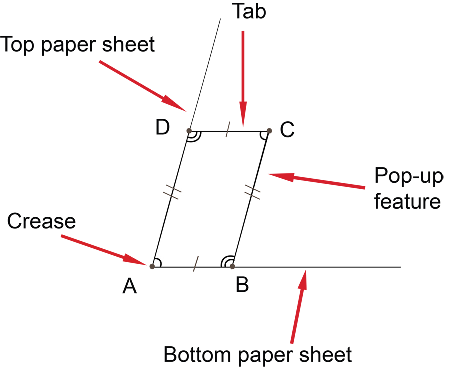
\includegraphics{figures/shared/01_Background/popup-diagram.pdf}
\caption{Cross-section of a popup card Figure modified from
https://en.wikipedia.org/wiki/File:Popup-diagram.svg.}
\end{figure}

The 90-degree popup card presents a tightly-constrained problem, with
opportunities for both interface design and algorithm innovations. We
present a system for designing popup cards, whose audience is
deliberately broad. We aim to make the pop=up card design process easier
and more fun.

Typically, users create popup cards through manual methods. For example,
a user might sketch out shape on a card in pencil, and then measure with
a rule to find locations to place folds. Or, they might \footnote{These
  are behaviors we observed by watching users create pop-up cards.}

\section{Motivation}\label{motivation}

\emph{This section is co-authored with Marissa Allen}

\begin{figure}[htbp]
\centering
\includegraphics{figures/shared/02_Overview/allcards.pdf}
\caption{A sample of cards created using Foldlings. For larger images
and fold patterns, see \nameref{appendix-d-sample-cards} on page
\pageref{appendix-d-sample-cards}.}
\end{figure}

We set out to create a tool that would help people design 3D pop-up
cards. We were driven by the desire to create original kirigami designs
without a template. As we progressed in our project, we began to focus
on developing a tool that would provide a way to create pop-ups more
intuitively, without explicitly understanding how to create a valid
90-degree pop-up card. Our tool allows users to design, iterate, and
preview an original pop-up card before they even pick up a pair of
scissors.

We outline some user stories --- potential use cases for our software:

\begin{itemize}
\itemsep1pt\parskip0pt\parsep0pt
\item
  George is an avid scrapbooker. He uses Foldlings to create small
  pop-up elements to liven up his scrapbooks. Sometimes he, creates
  cards to commemorate moments --- other times, he pastes photos or
  other media onto a pop-up card structure created with our app.
\item
  Sally designs cards for a commercial greeting card company. She uses
  Foldlings to create rough prototypes and concept sketches for pop-up
  cards. After getting feedback from the rest of her team, she brings
  the exported SVG file into Adobe Illustrator to refine the final card
  designs.
\item
  Jim forgot to make a card for his wife's anniversary present, and
  she's coming home in an hour! He downloads Foldlings from the Apple
  App Store, and is able to quickly design and create a beautiful card.
\item
  Alex is a creative college student who wants to continue making things
  for her friends and family. She wants to explore pop-up cards, but
  doesn't like any of the templates she's found online and can't pay for
  pop-up design books. She finds Foldlings in the Apple App Store and
  tests her creativity with our tool.
\item
  Kate, a middle school math teacher, is teaching a module on pop-up
  card geometry. She uses Foldlings to teach the students about the
  parallelogram constraints between planes as cards fold. By using our
  app, her students gain an intuitive understanding of the geometric
  constraints.
\end{itemize}

\section{Technical Overview}\label{technical-overview}

\emph{This section is co-authored with Marissa Allen}

Our algorithmic simulation and validity detection is based on a tight
set of constraints to the pop-up card problem. We require the card to
have a central main valley fold --- from there we can determine the
orientation of planes, as alternating folds fold in opposite
orientations. The card then folds 180 degrees; this implies
parallelogram constraints between all the edges in a sideways
cross-section (with the exception of v-fold features).

We capture touch input, translating touches into cuts and folds
depending on the geometry of the fold feature. We validate fold features
before they are added to the sketch, ensuring that the design can fold
in 3D. At this point, we also perform bezier path operations to modify
existing edges in the sketch based on the new design element. When a
fold feature is added to the sketch, we re-calculate planes (areas
enclosed by cuts and folds) by traversing a directed graph of edges in
the sketch. Based on these 2D planes, we create 3D planes, which are
oriented and translated based on their relationship to other planes in
the sketch. In 3D, we animate planes in response to user input. Each of
the planes is translated in relation to the plane oriented above the
fold and rotated in relation to the main driving joint.

Our approach constructs a tree representation of the planes based on
fold adjacency and uses this for determining the parent child
relationships in the simulated 3D view. We also use a tree-based
structure to store associations between logical geometric units.

\subsection{Development Process}\label{development-process}

\begin{figure}[htbp]
\centering
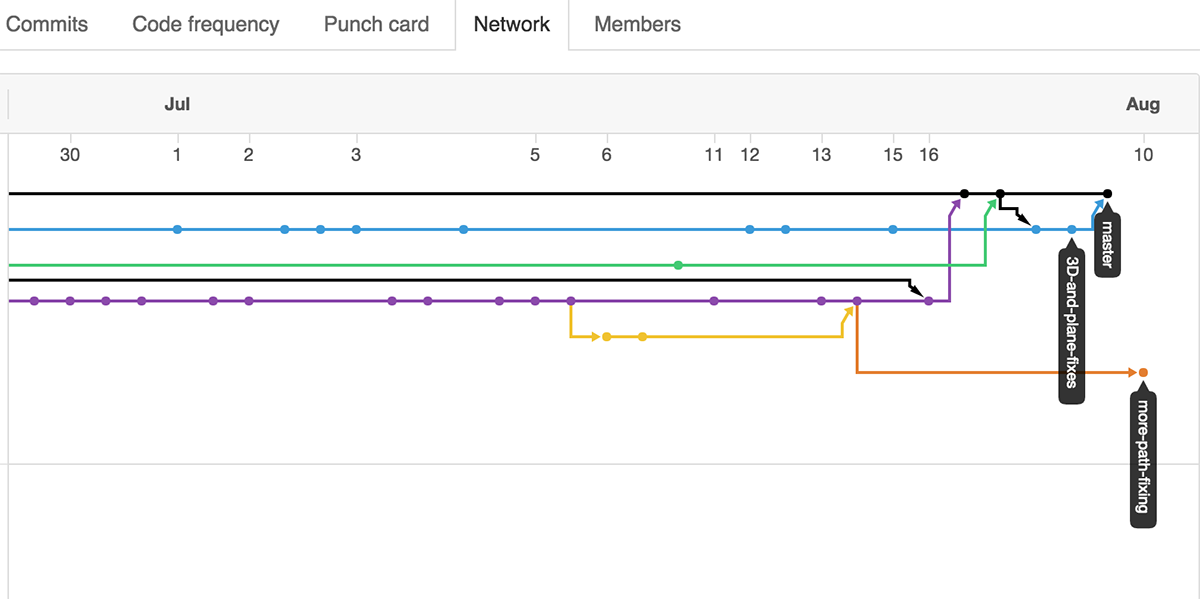
\includegraphics{figures/shared/02_Overview/gitflow.png}
\caption{Branches in our github.com repository.}
\end{figure}

We designed and developed the software interactively, frequently testing
prototypes with users. We used github to build Foldlings
collaboratively. Our workflow involved creating new code branches for
each feature, and reviewing the changes before merging back into the
master branch of the codebase. The full source for our software is
available at \url{http://github.com/harquail/foldlings/}.

\section{Pipeline Overview}\label{pipeline-overview}

\emph{This section is co-authored with Marissa Allen}

\begin{figure}[htbp]
\centering
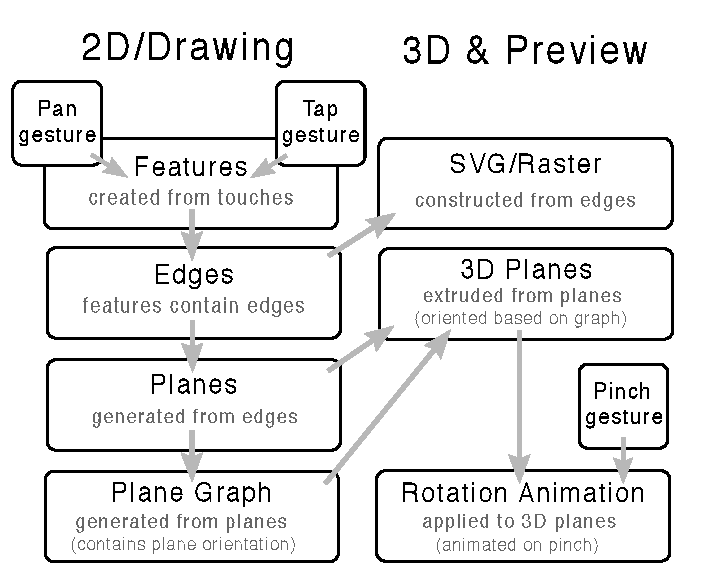
\includegraphics{figures/shared/02_Overview/pipeline.pdf}
\caption{Overview of data flow between 2D and 3D systems.}
\end{figure}

To begin, a user draws a design using the fold feature tools: box fold,
polygon, freeform and v-fold. These tools create a pattern of cuts and
folds, displaying an interactive preview of the design as the user
creates it. The cuts and folds created with these tools remain
associated with each other, and can be modified or deleted as a unit.

Each time a new shape is added to the design, it is evaluated for
validity: whether it can fold to 90 degrees and be parsed into
individual planes. The planes are then linked together in an acyclic
graph based on the planes' abutting top edges. This acyclic graph allows
us to shade planes based on orientation in 2D and simulate the design in
3D. Each feature can also be modified or deleted, by tapping on the
feature an selecting an entry from the list of available options.

This process continues until the user previews the design in 3D. The 3D
preview displays a simulation of how the design will fold, which can be
manipulated using a pinch gesture. The user is free to return to the 2D
drawing interface and continue editing his/her design or save the design
as either a raster file or SVG vector file. After this step, the user
can print and cut the raster file or open the SVG file on a laser cutter
or other cutting tool. We automatically save designs locally when
leaving the design workspace, so users can restore their work.

Figure 1.6 shows the full pipeline for designing cards. It shows a
user's design process, starting with concept sketches, and moving
through iterations of the sketch using the 3D preview to test the
design. Finally, the user exports the design as a fold pattern, and cuts
and folds the pop-up card.

\begin{figure}[htbp]
\centering
\includegraphics{figures/shared/02_Overview/sinewave.pdf}
\caption{A full outline of the design process for Foldlings, from
initial concept sketches to full realization of a paper pop-up card.}
\end{figure}

\section{Related Work}\label{related-work}

\textbf{\textgreater{}\textgreater{}TODO: Complete w/Marissa}

\emph{This section is co-authored with Marissa Allen}

Our approach to pop-up creation does not require glue or 3D modeling
experience, but is more similar to kirigami. Glue-based design presents
different affordances than kirigami, but requires an assembly stage that
disconnects the initial 2D pattern from the final pop-up geometry
{[}Glassner 1998{]}. Others approach the pop-up design problem from the
opposite direction: creating designs by modeling in 3D space {[}Ruiz et
al. 2014{]}. {[}Li et al. 2010{]} transform 3D models into paper
architectures that are stable and rigid. A drawback to this approach is
that it does not preserve the original model's features. Compared to
existing tools, Foldlings allows novice users more opportunities for
free-form, artistic expression in the pop-up medium.

There has been prior work done on automated methods to create a pop-up
schematic. For example, Li, Xian-Ying, et al. develop an algorithm that
transforms user-defined models into paper architectures that are stable
and rigid. Because their algorithm modifies the input geometry given by
the user, the end result does not preserve the original model's
features. Other attempts to create pop-up cards such as Abel, Zachary,
et al. --- can only take in simple polygonal meshes and require the user
to fold and glue additional pieces of paper together, whereas our
approach creates a pop-up card with arbitrary shapes from a single piece
of paper. These methods also impose strict constraints on user input,
which requires the end user to know how to model an object in 3D and
thus is not accessible to novice users.

Our approach to smoothing user input as the user draws his/her design is
similar to Johnson, Gabe, et al. After a user has drawn lines in their
program, they edit these lines depending on what mode the user is in and
the drawing is then sent to a laser-cutter. However, our method
automatically interpolates the lines given by the user and transforms
them into smoothed Bezier curves, ready to be printed.

Hendrix, Susan L., and Michael Eisenberg. ``Computer-assisted pop-up
design for children: computationally enriched paper engineering.''
Advanced Technology for Learning 3.2 (2006): 119-127.
\citet{hendrix2006computer}

The pop-up tool described by this paper is very similar to our current
design. However, this tool was built as an introduction to the
engineering sciences and not as a tool to aid artistic design. Perhaps
as a result of an engineering-centric design methodology, the pop-up
tool has a more restrictive UI than ours. Their program is designed to
only create the simple folding mechanism of the pop-up card. Adding
arbitrary cuts and multiple layers is not supported and must be added
later.

Okamura, Sosuke, and Takeo Igarashi. ``An interface for assisting the
design and production of pop-up card.'' Smart Graphics. Springer Berlin
Heidelberg, 2009. \citet{okamura2009interface}

This paper describes a program to design elaborate 180º pop-ups that can
be applied to both cards and books strictly within a 3d environment.
Their manufacturing process is additive, using glue to connect the
pieces. They implement collision testing and multiple components inside
their pop-up program. However, their program does not incorporate the
main folding piece in designing their pop-ups, it is simply a mechanical
driver for the rest of the design. Therefore, a user cannot design a
pop-up that consists of only one piece of paper that does not require
gluing.

Way, Der-Lor, Yong-Ning Hu, and Zen-Chung Shih. ``The Creation of V-fold
Animal Pop-Up Cards from 3D Models Using a Directed Acyclic
Graph.''Advances in Intelligent Systems and Applications-Volume 2.
Springer Berlin Heidelberg, 2013. 465-475. \citet{way2013creation}

The tool described in this paper creates pop-ups from 3d models. The
tool segments a 3d model and then uses shape recognition to create paper
models in pop-up cards. The authors create an acyclic graph from these
segments and use the nodes to drive a simulation of the pieces based on
opening and closing the card. This paper has a similar simulation
technique to our approach. However, they generate their designs from 3d
shapes instead of 2d patterns.

\section{Potential Applications}\label{potential-applications}

\emph{This section is co-authored with Marissa Allen}
\textbf{\textgreater{}\textgreater{}TODO: get comments/more content from
marissa}

As a general-purpose design tool for cuts and folds, Foldlings has a
wide variety of potential applications. For example, Melina Blees et al
present a graphene transistor that is constructed through kirigami
methods \citet{blees2014graphene}. Simple, usable interfaces for
designing complex kirigami structures are needed to advance similar
research.

One exciting application of Foldlings is as a tool for developing
advanced spatial reasoning skills. Taylor et al present a curriculum
that uses popup card design as a tool for building mathematics and
spatial reasoning skills \citet{taylor2013think3d}
\citet{olson_mathematics_2004}. A tool like Foldlings would likely
increase the effectiveness of such a program, since much of the
experimentation could happen more quickly in software than using manual
methods. Because our code is open source, advanced students could even
modify our software to develop new fold features and interactions.

\section{Appendix D: Separation of
Work}\label{appendix-d-separation-of-work}

I collaborated on this project with Marissa Allen. Although we worked
collaboratively on the software, each of us presents an individual
thesis paper. Our responsibilities on the software were as follows: Nook
concentrated on tools and interactions, including performing user
studies and processing user input, while Marissa concentrated on 3D
interactions and data structures, including the algorithms for shading
and traversing planes.

%END_INCLUDES

% \appendix
% 

\section*{Appendix A: User Study 1}
\addcontentsline{toc}{section}{Appendix A: User Study 1}

% \begin{figure}[h!]
% \begin{center}$
% \begin{array}{c c}
% 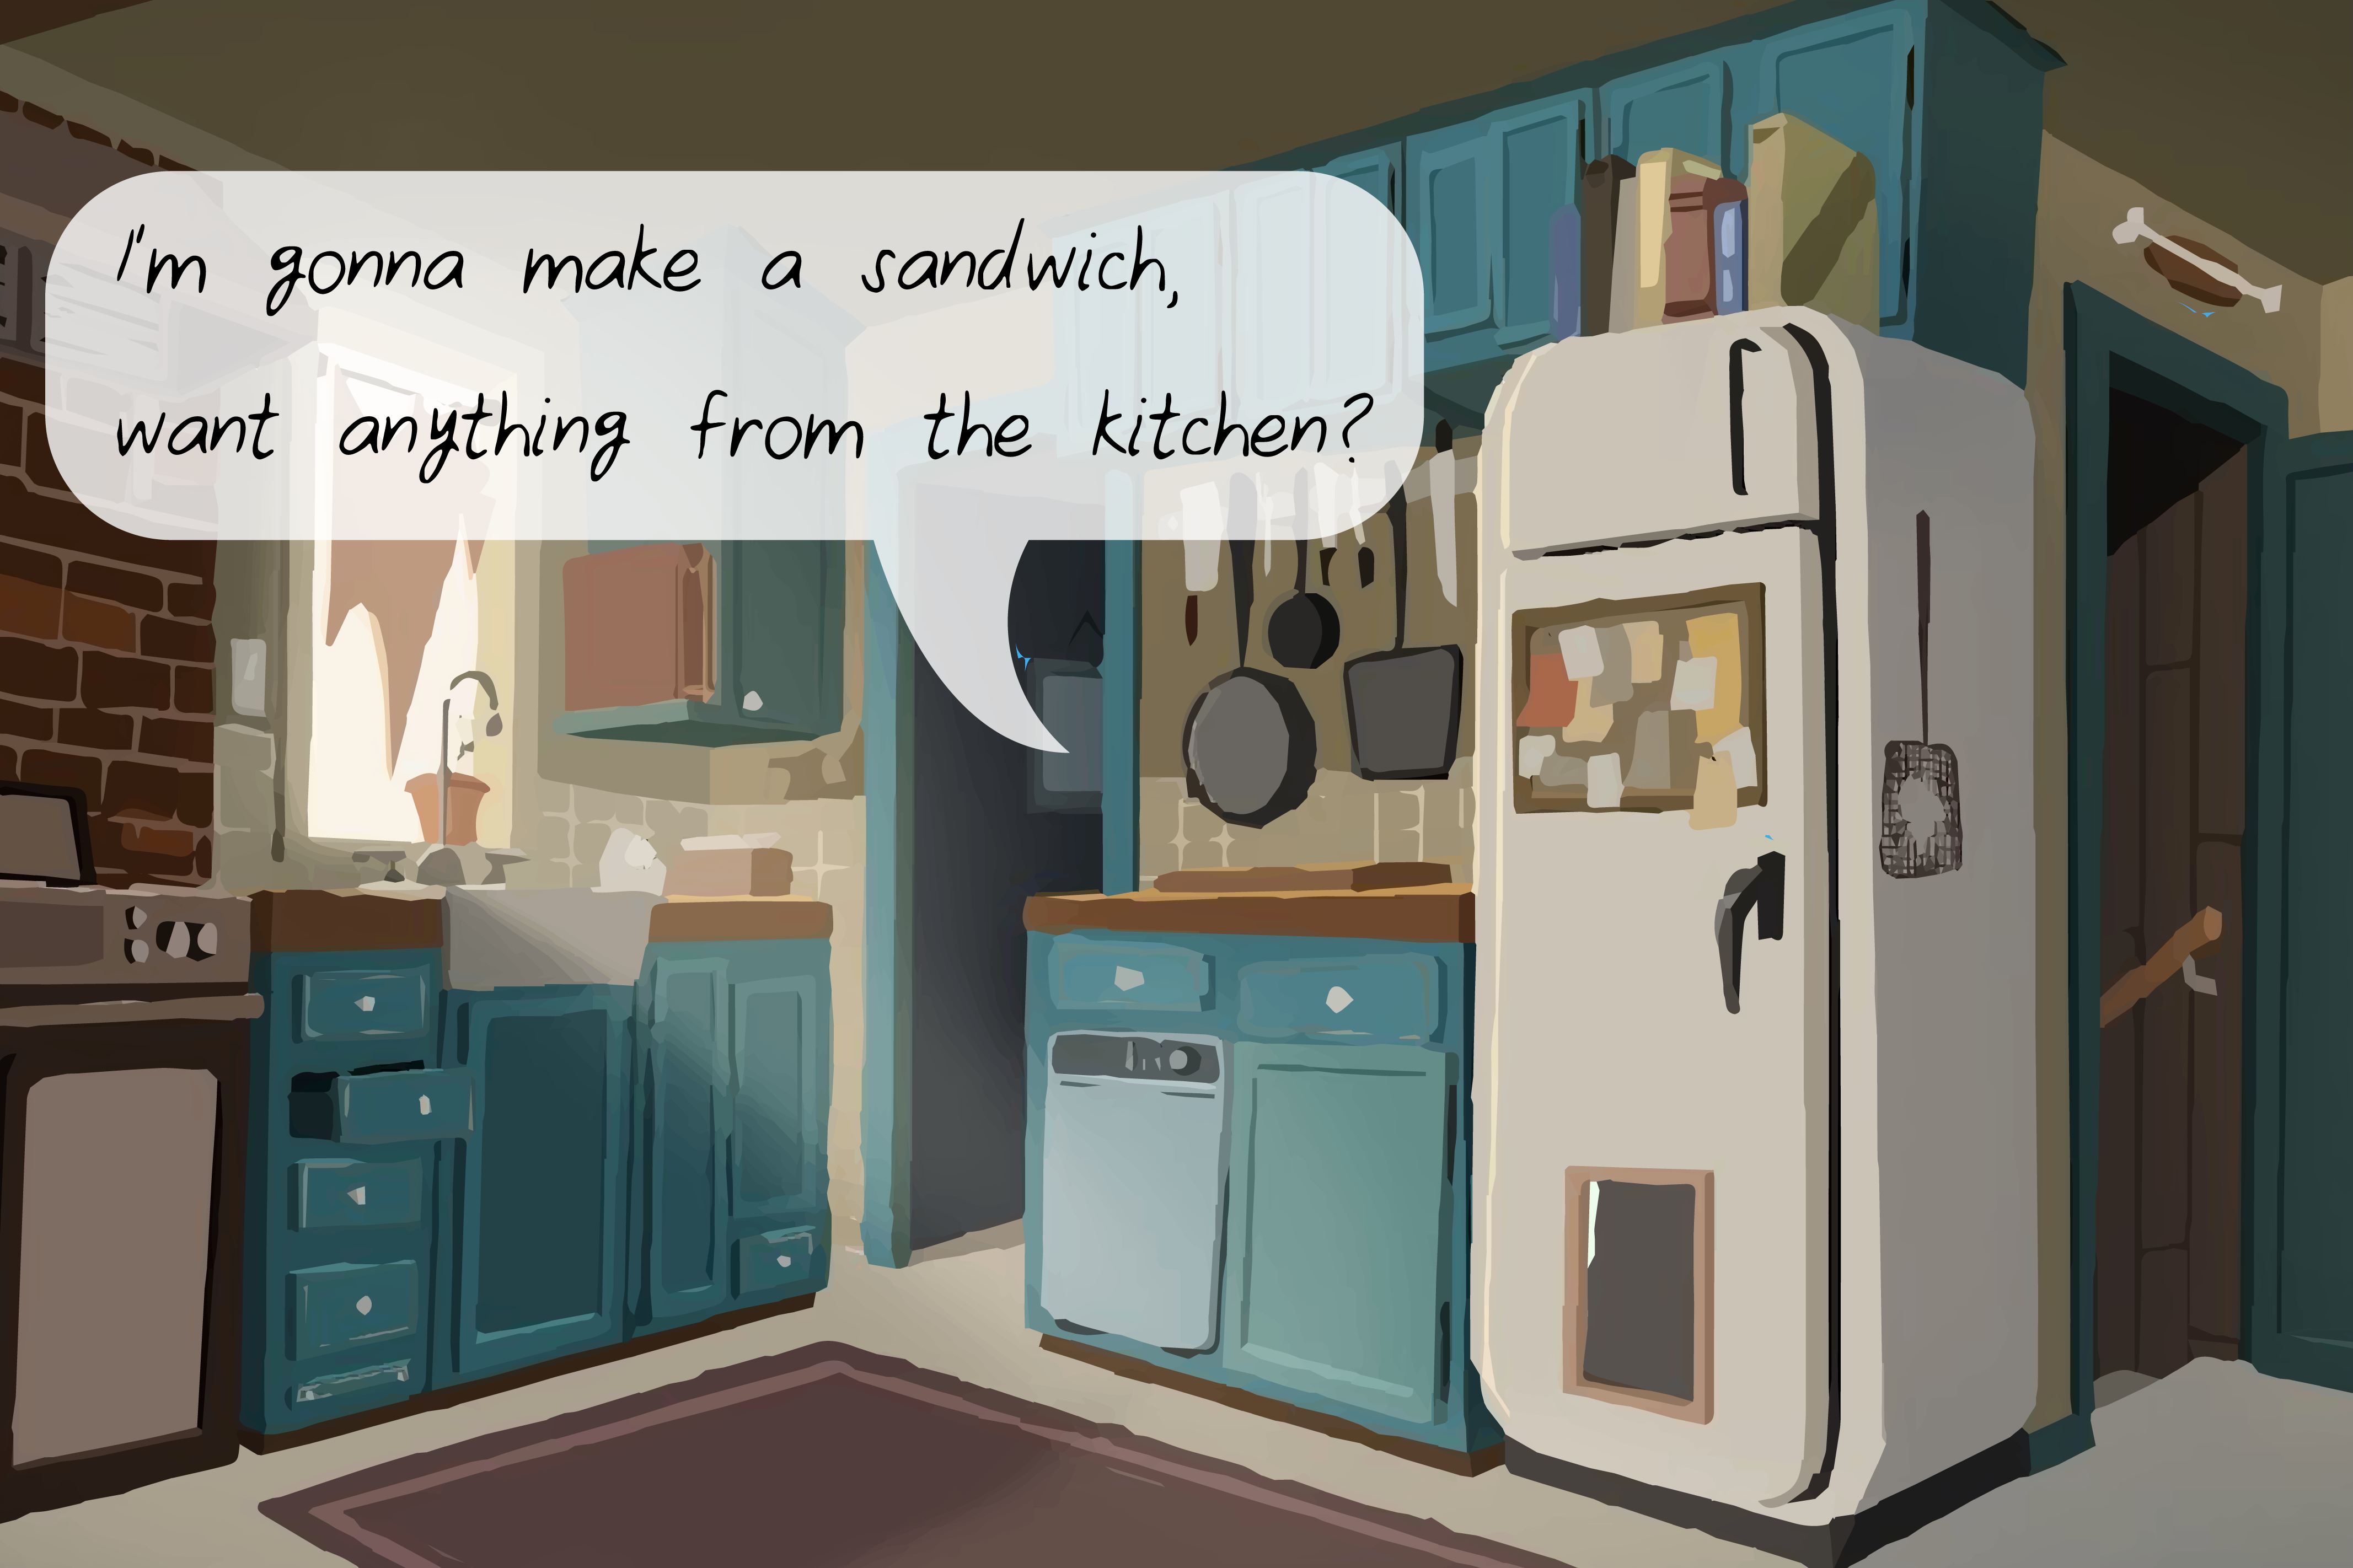
\includegraphics[width=2.3in]{figures/exp1/test-01.png} &
% 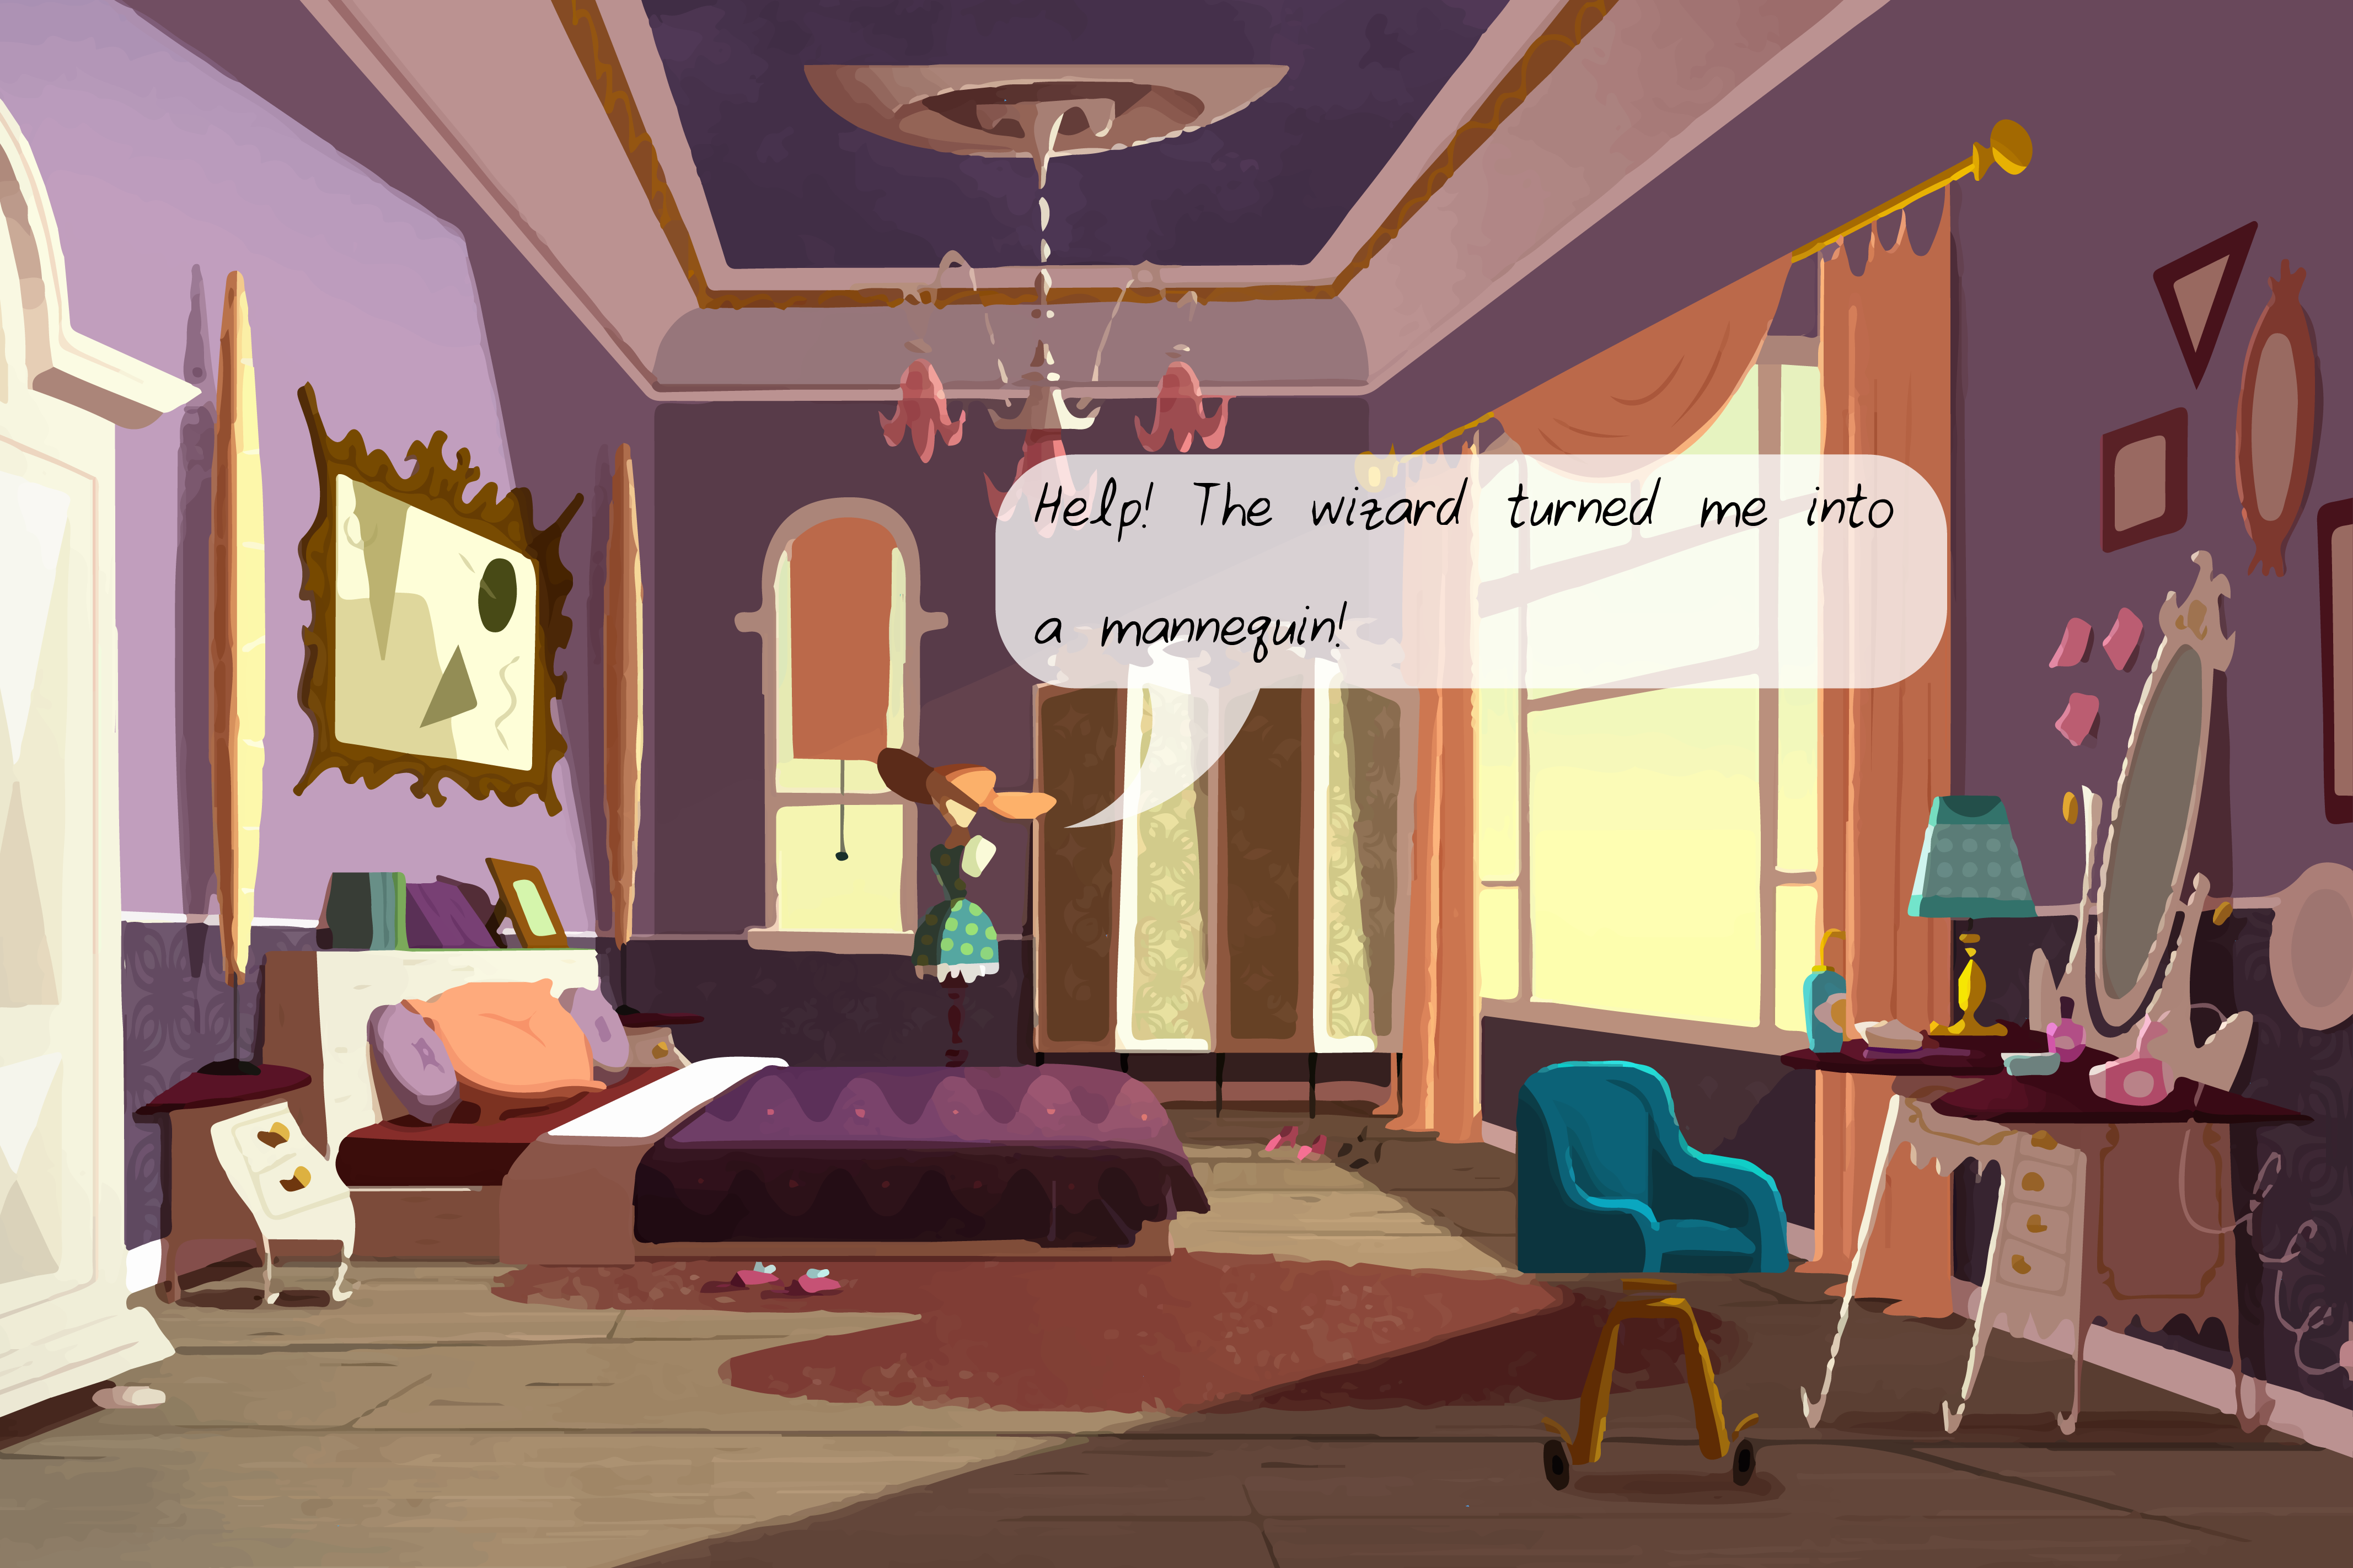
\includegraphics[width=2.3in]{figures/exp1/test-02.png} \\ 
% 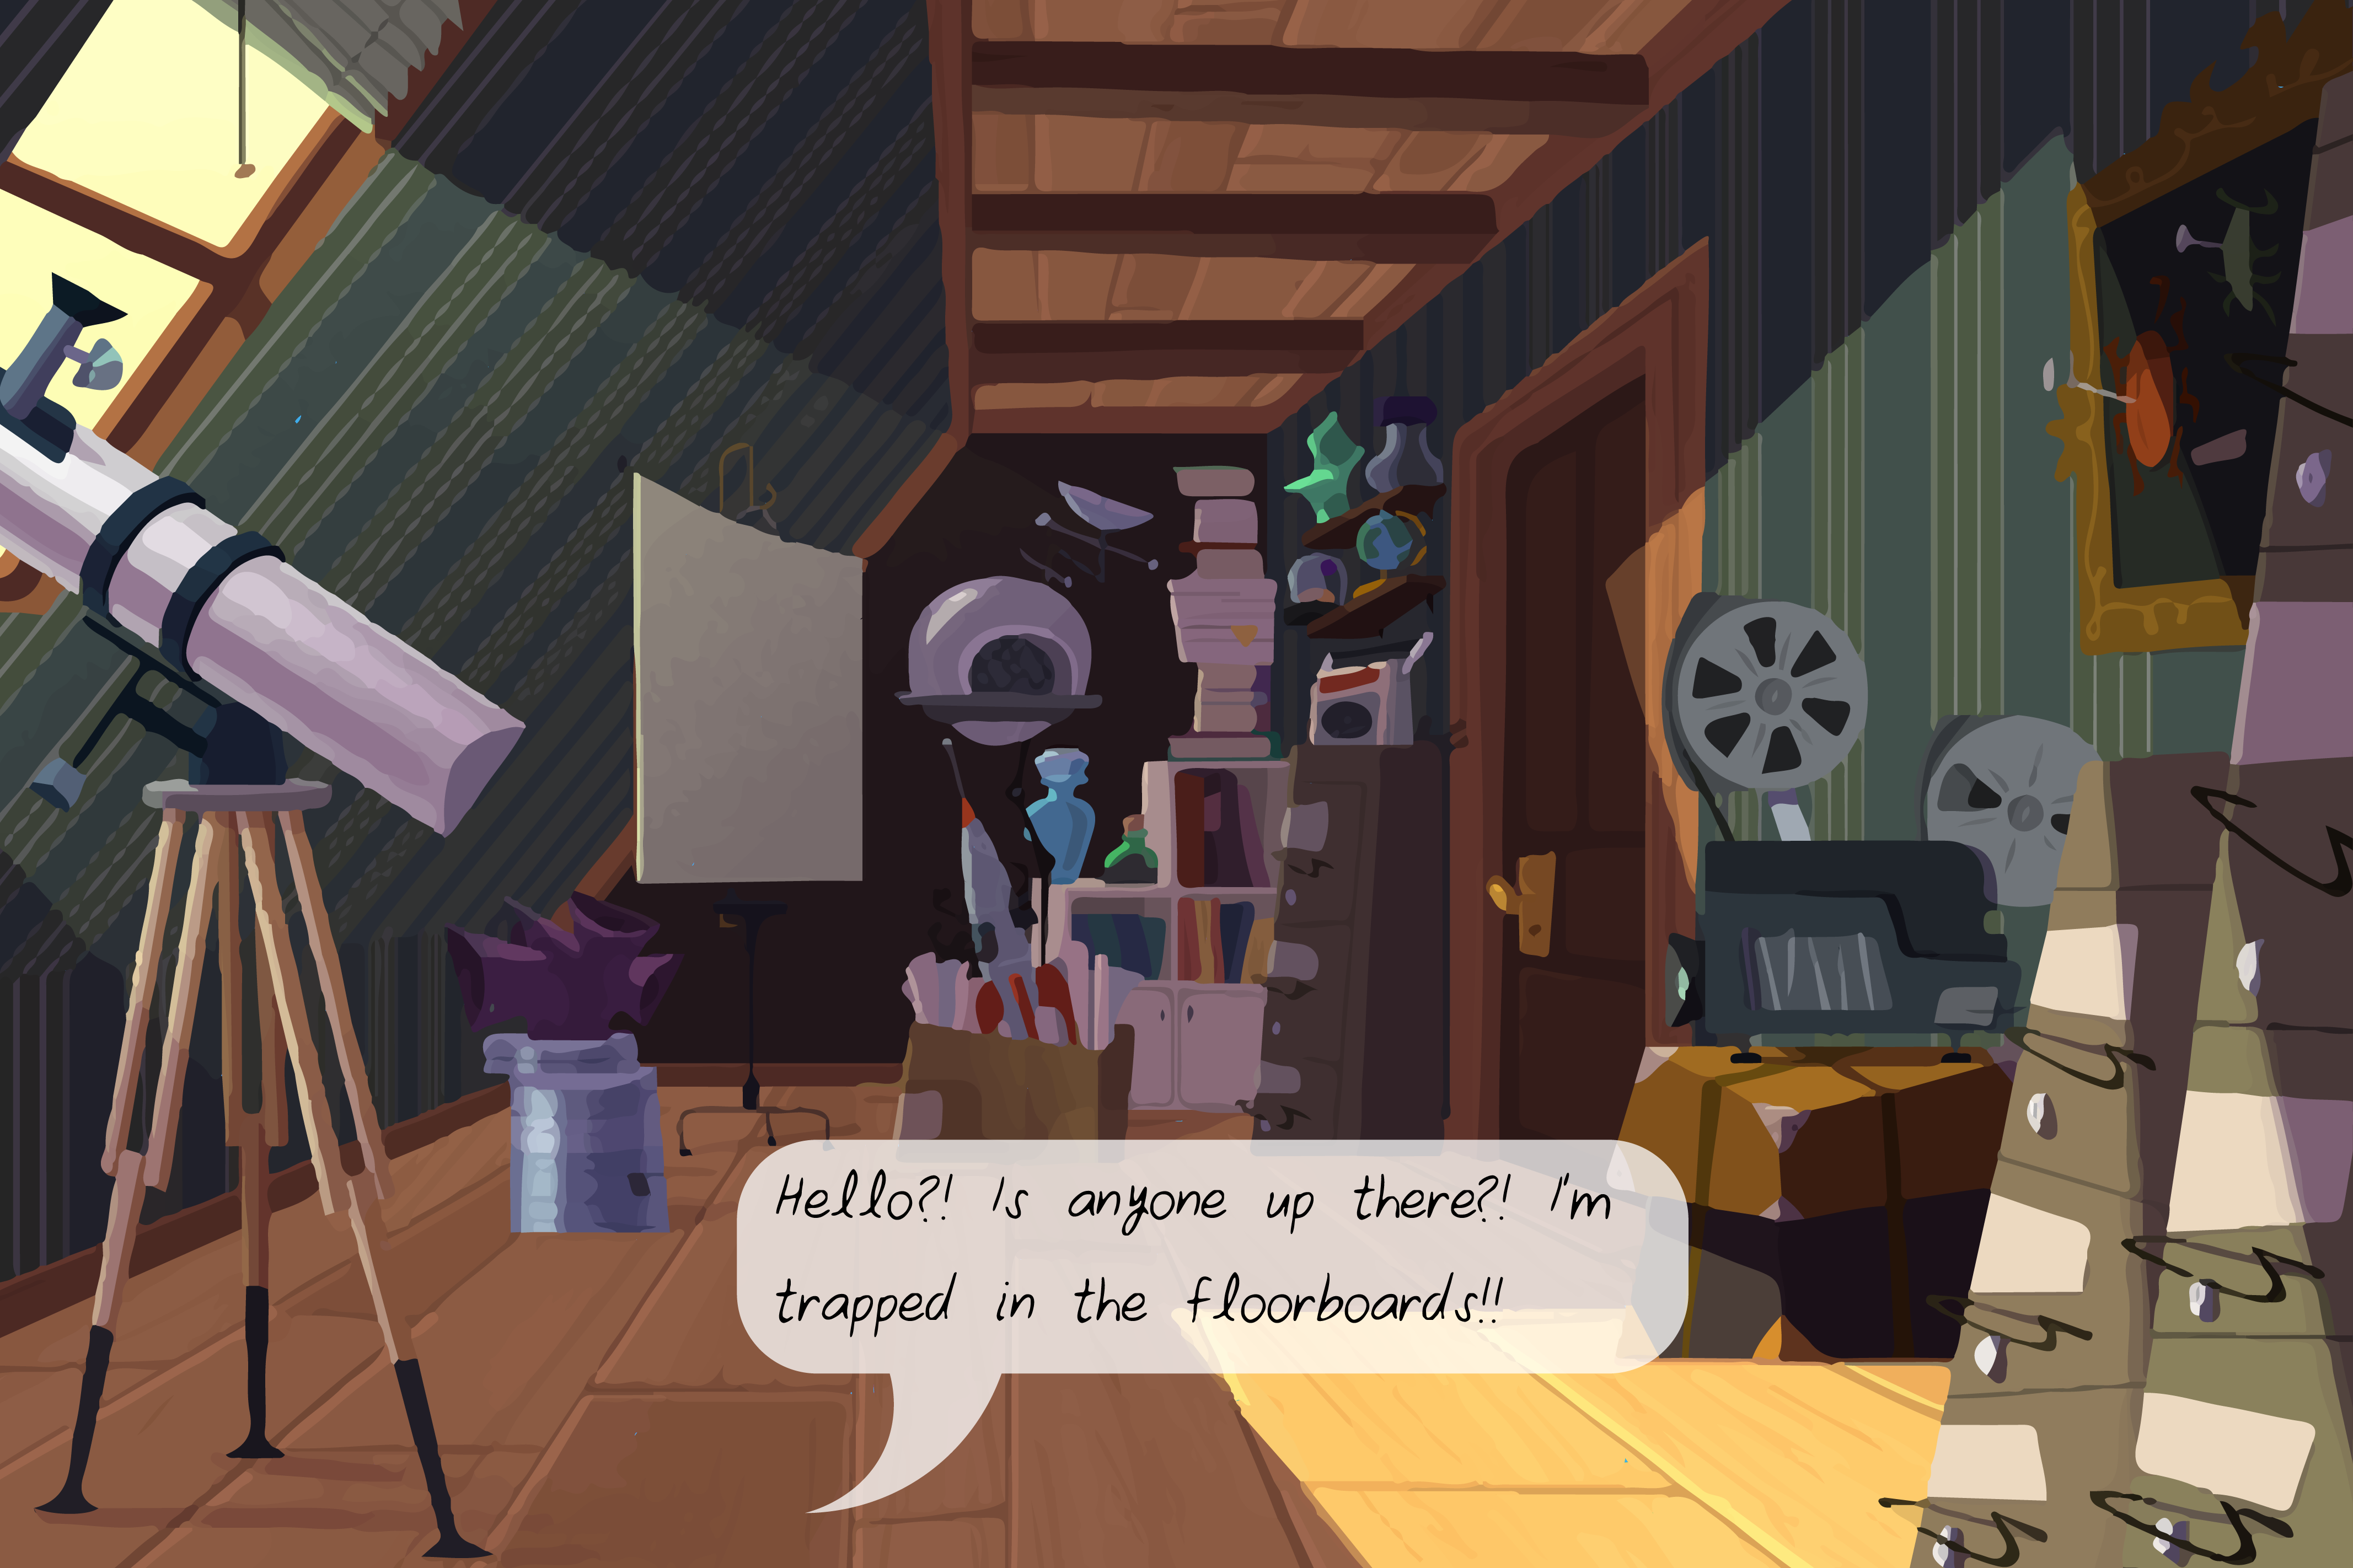
\includegraphics[width=2.3in]{figures/exp1/test-03.png} &
% 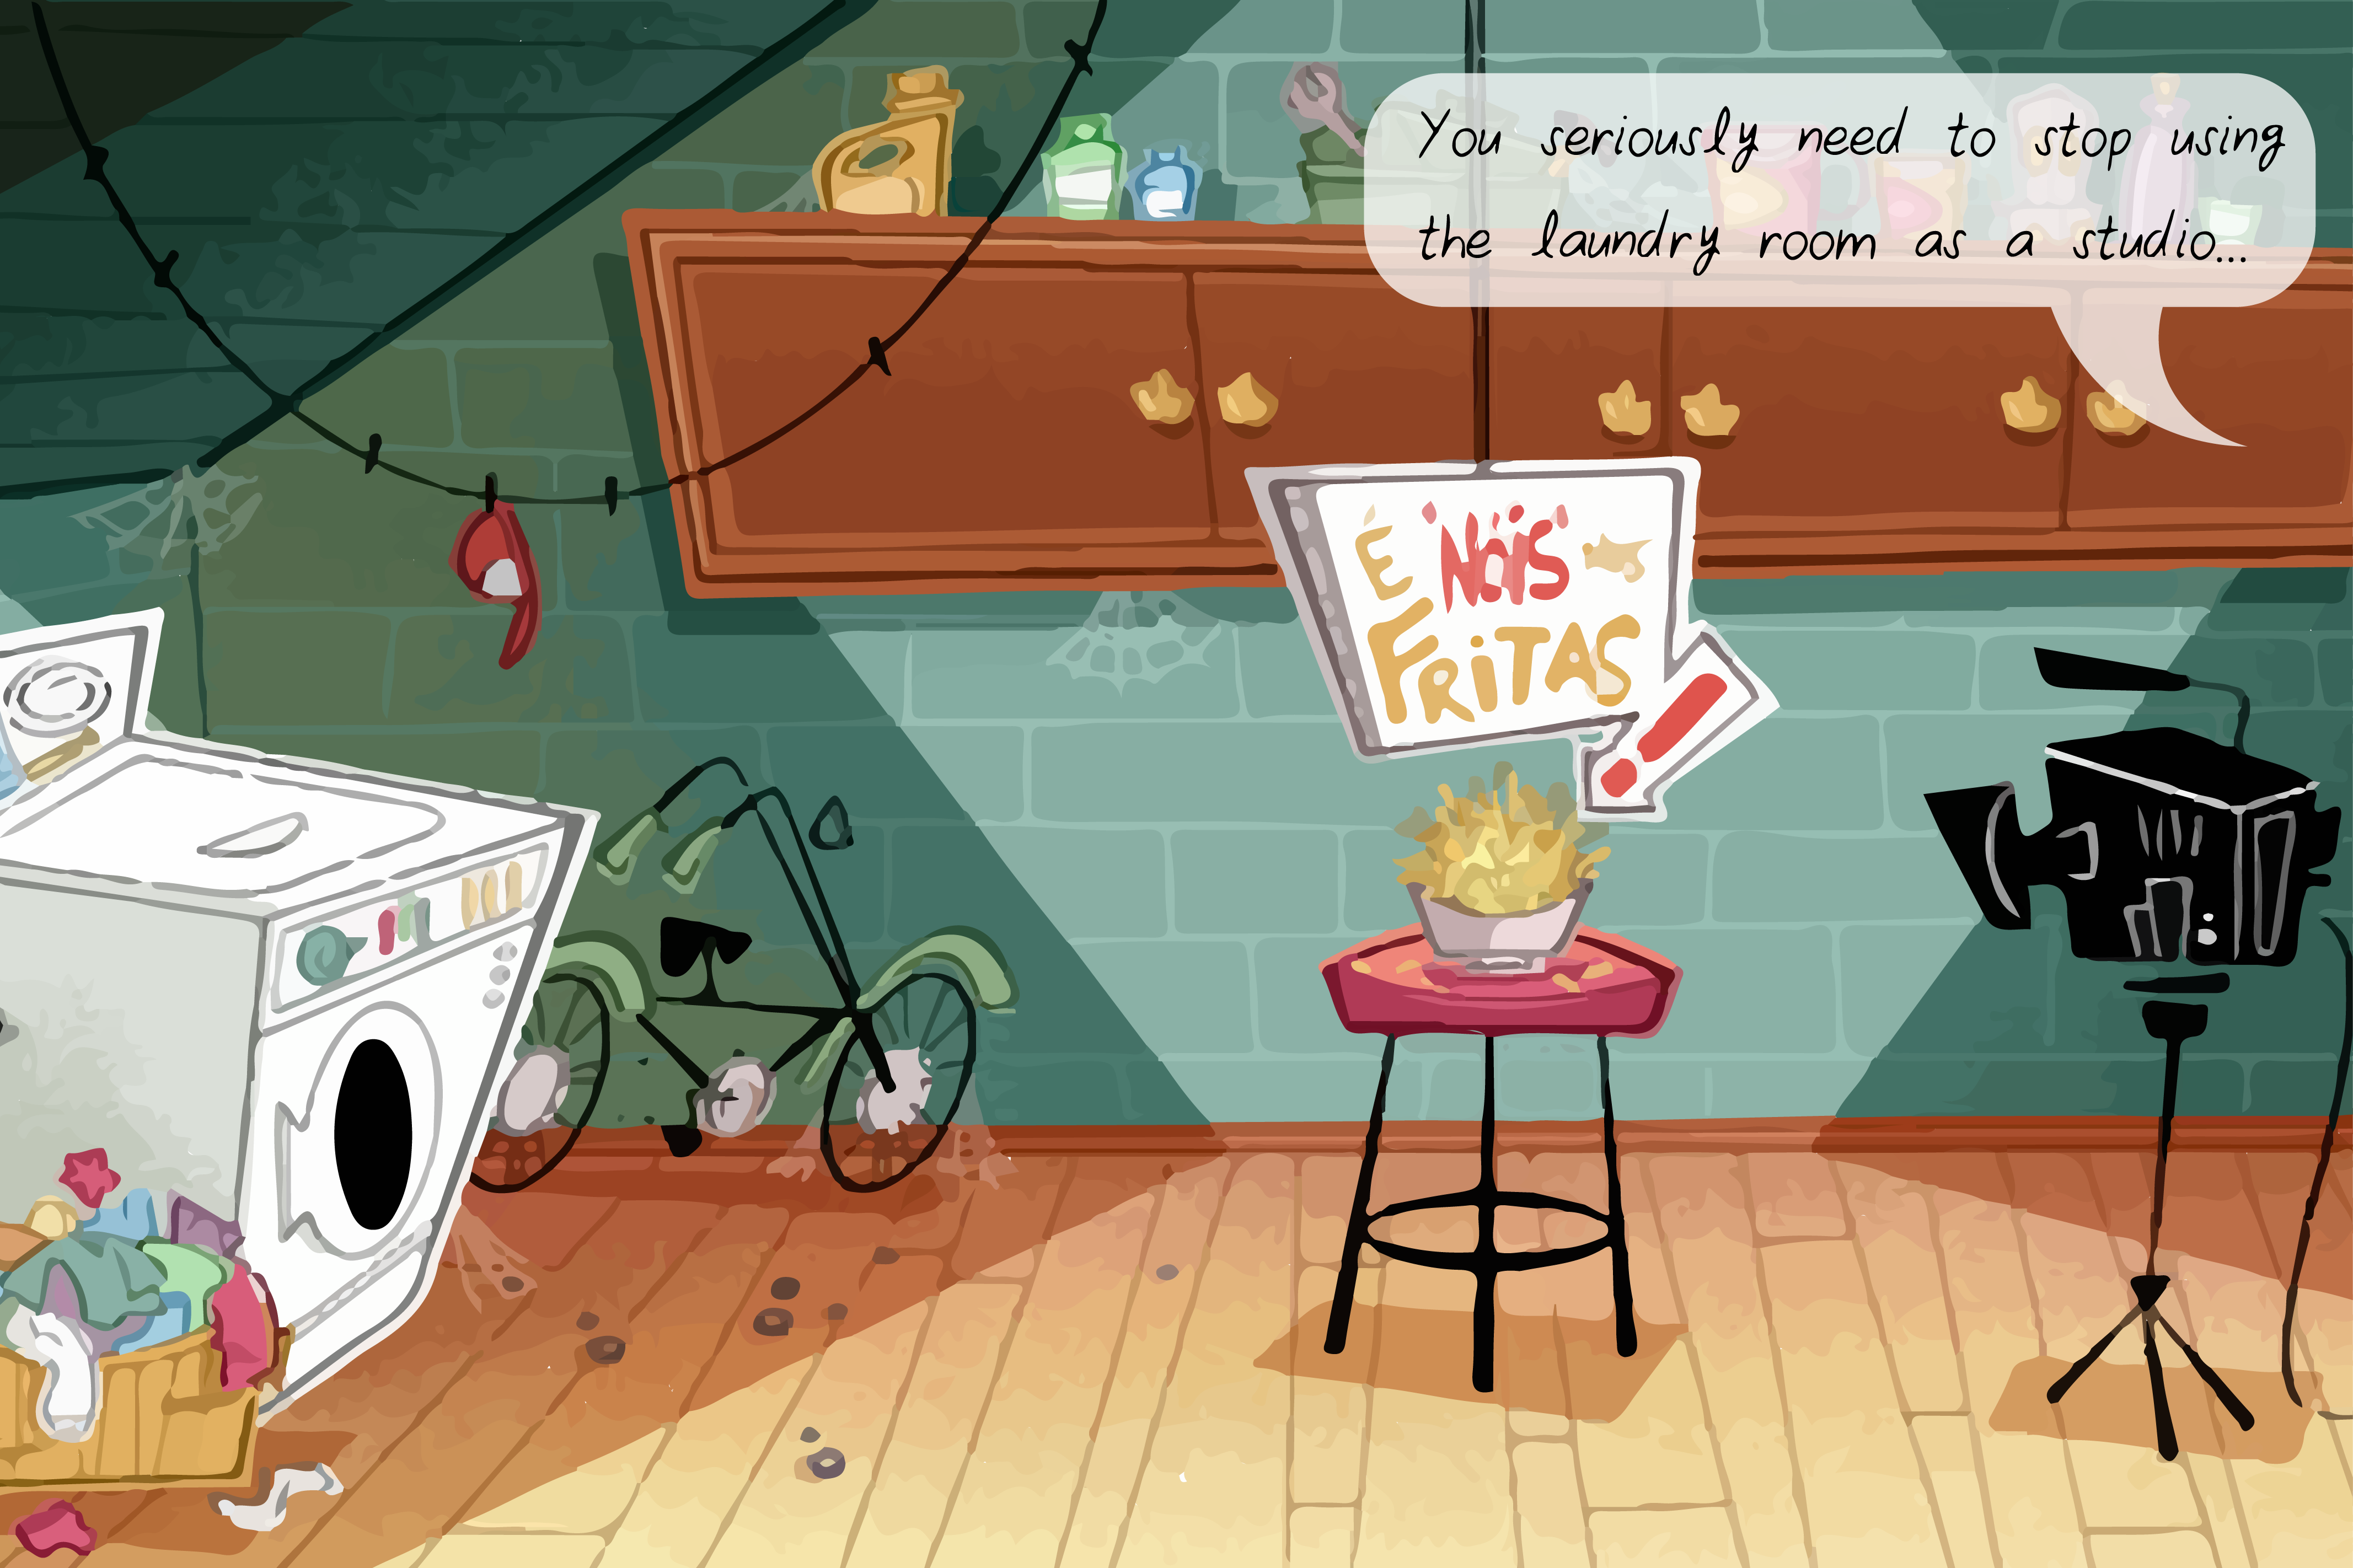
\includegraphics[width=2.3in]{figures/exp1/test-04.png} \\ 
% 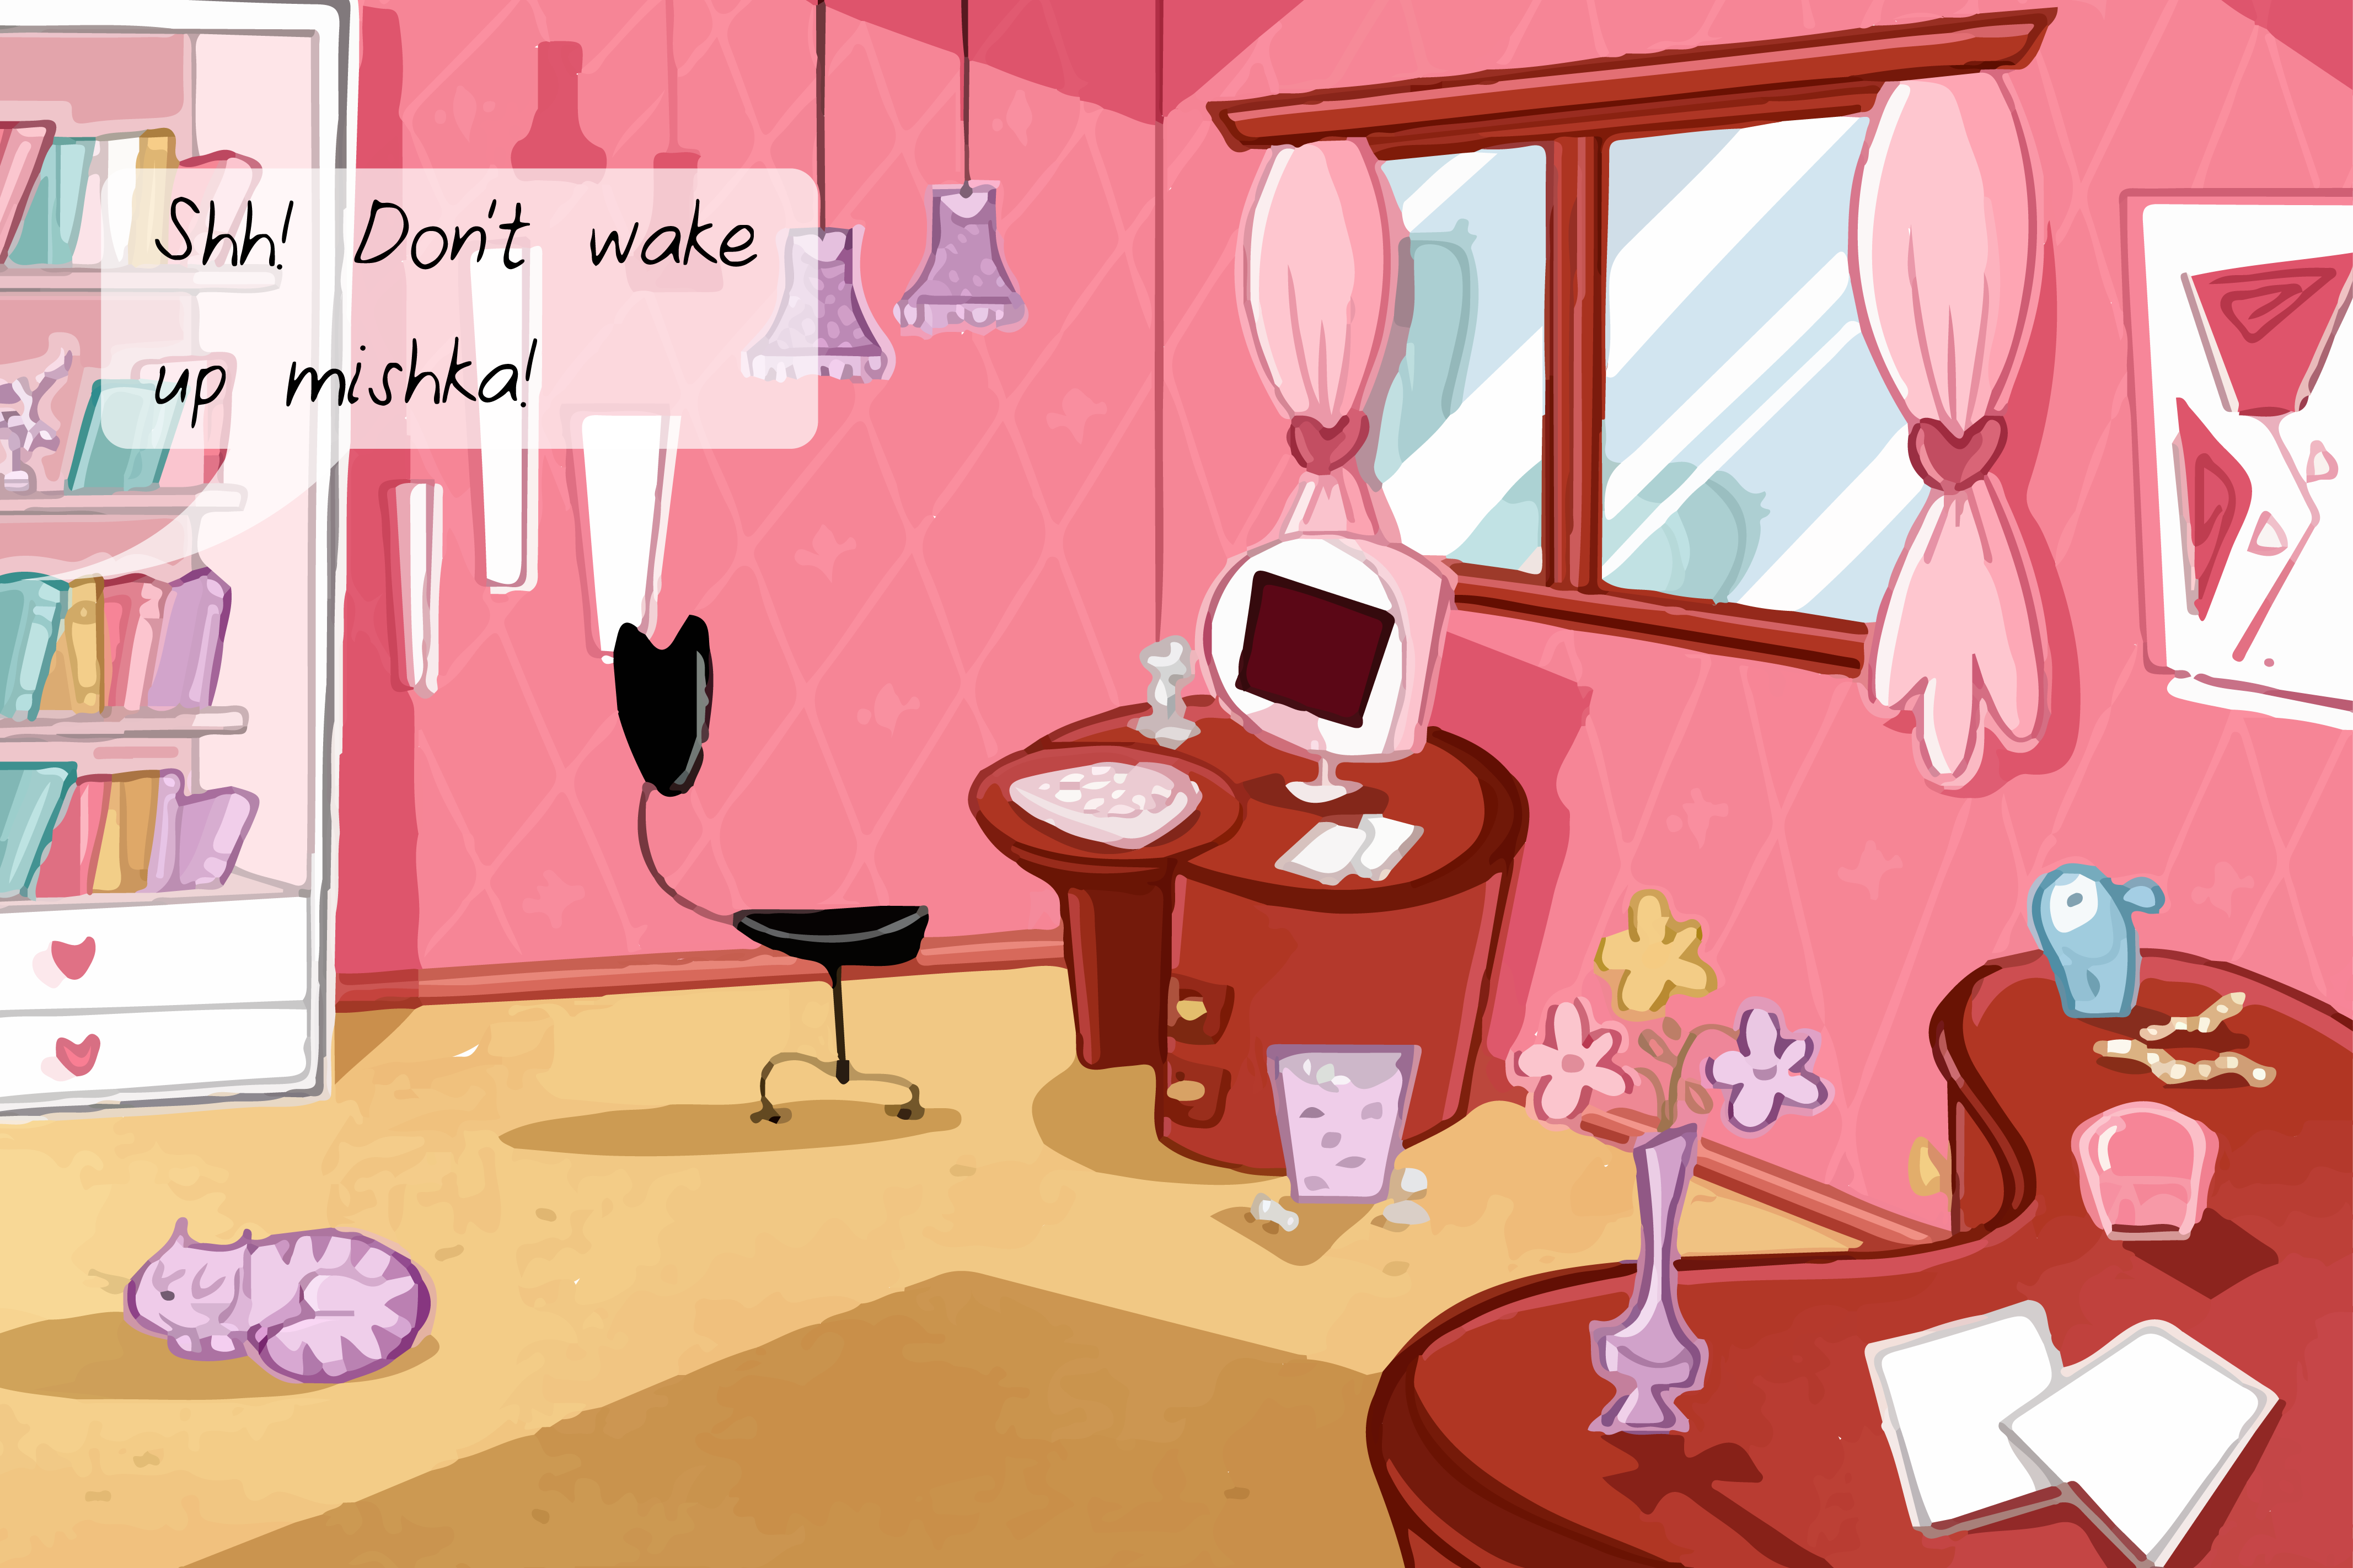
\includegraphics[width=2.3in]{figures/exp1/test-05.png} &
% 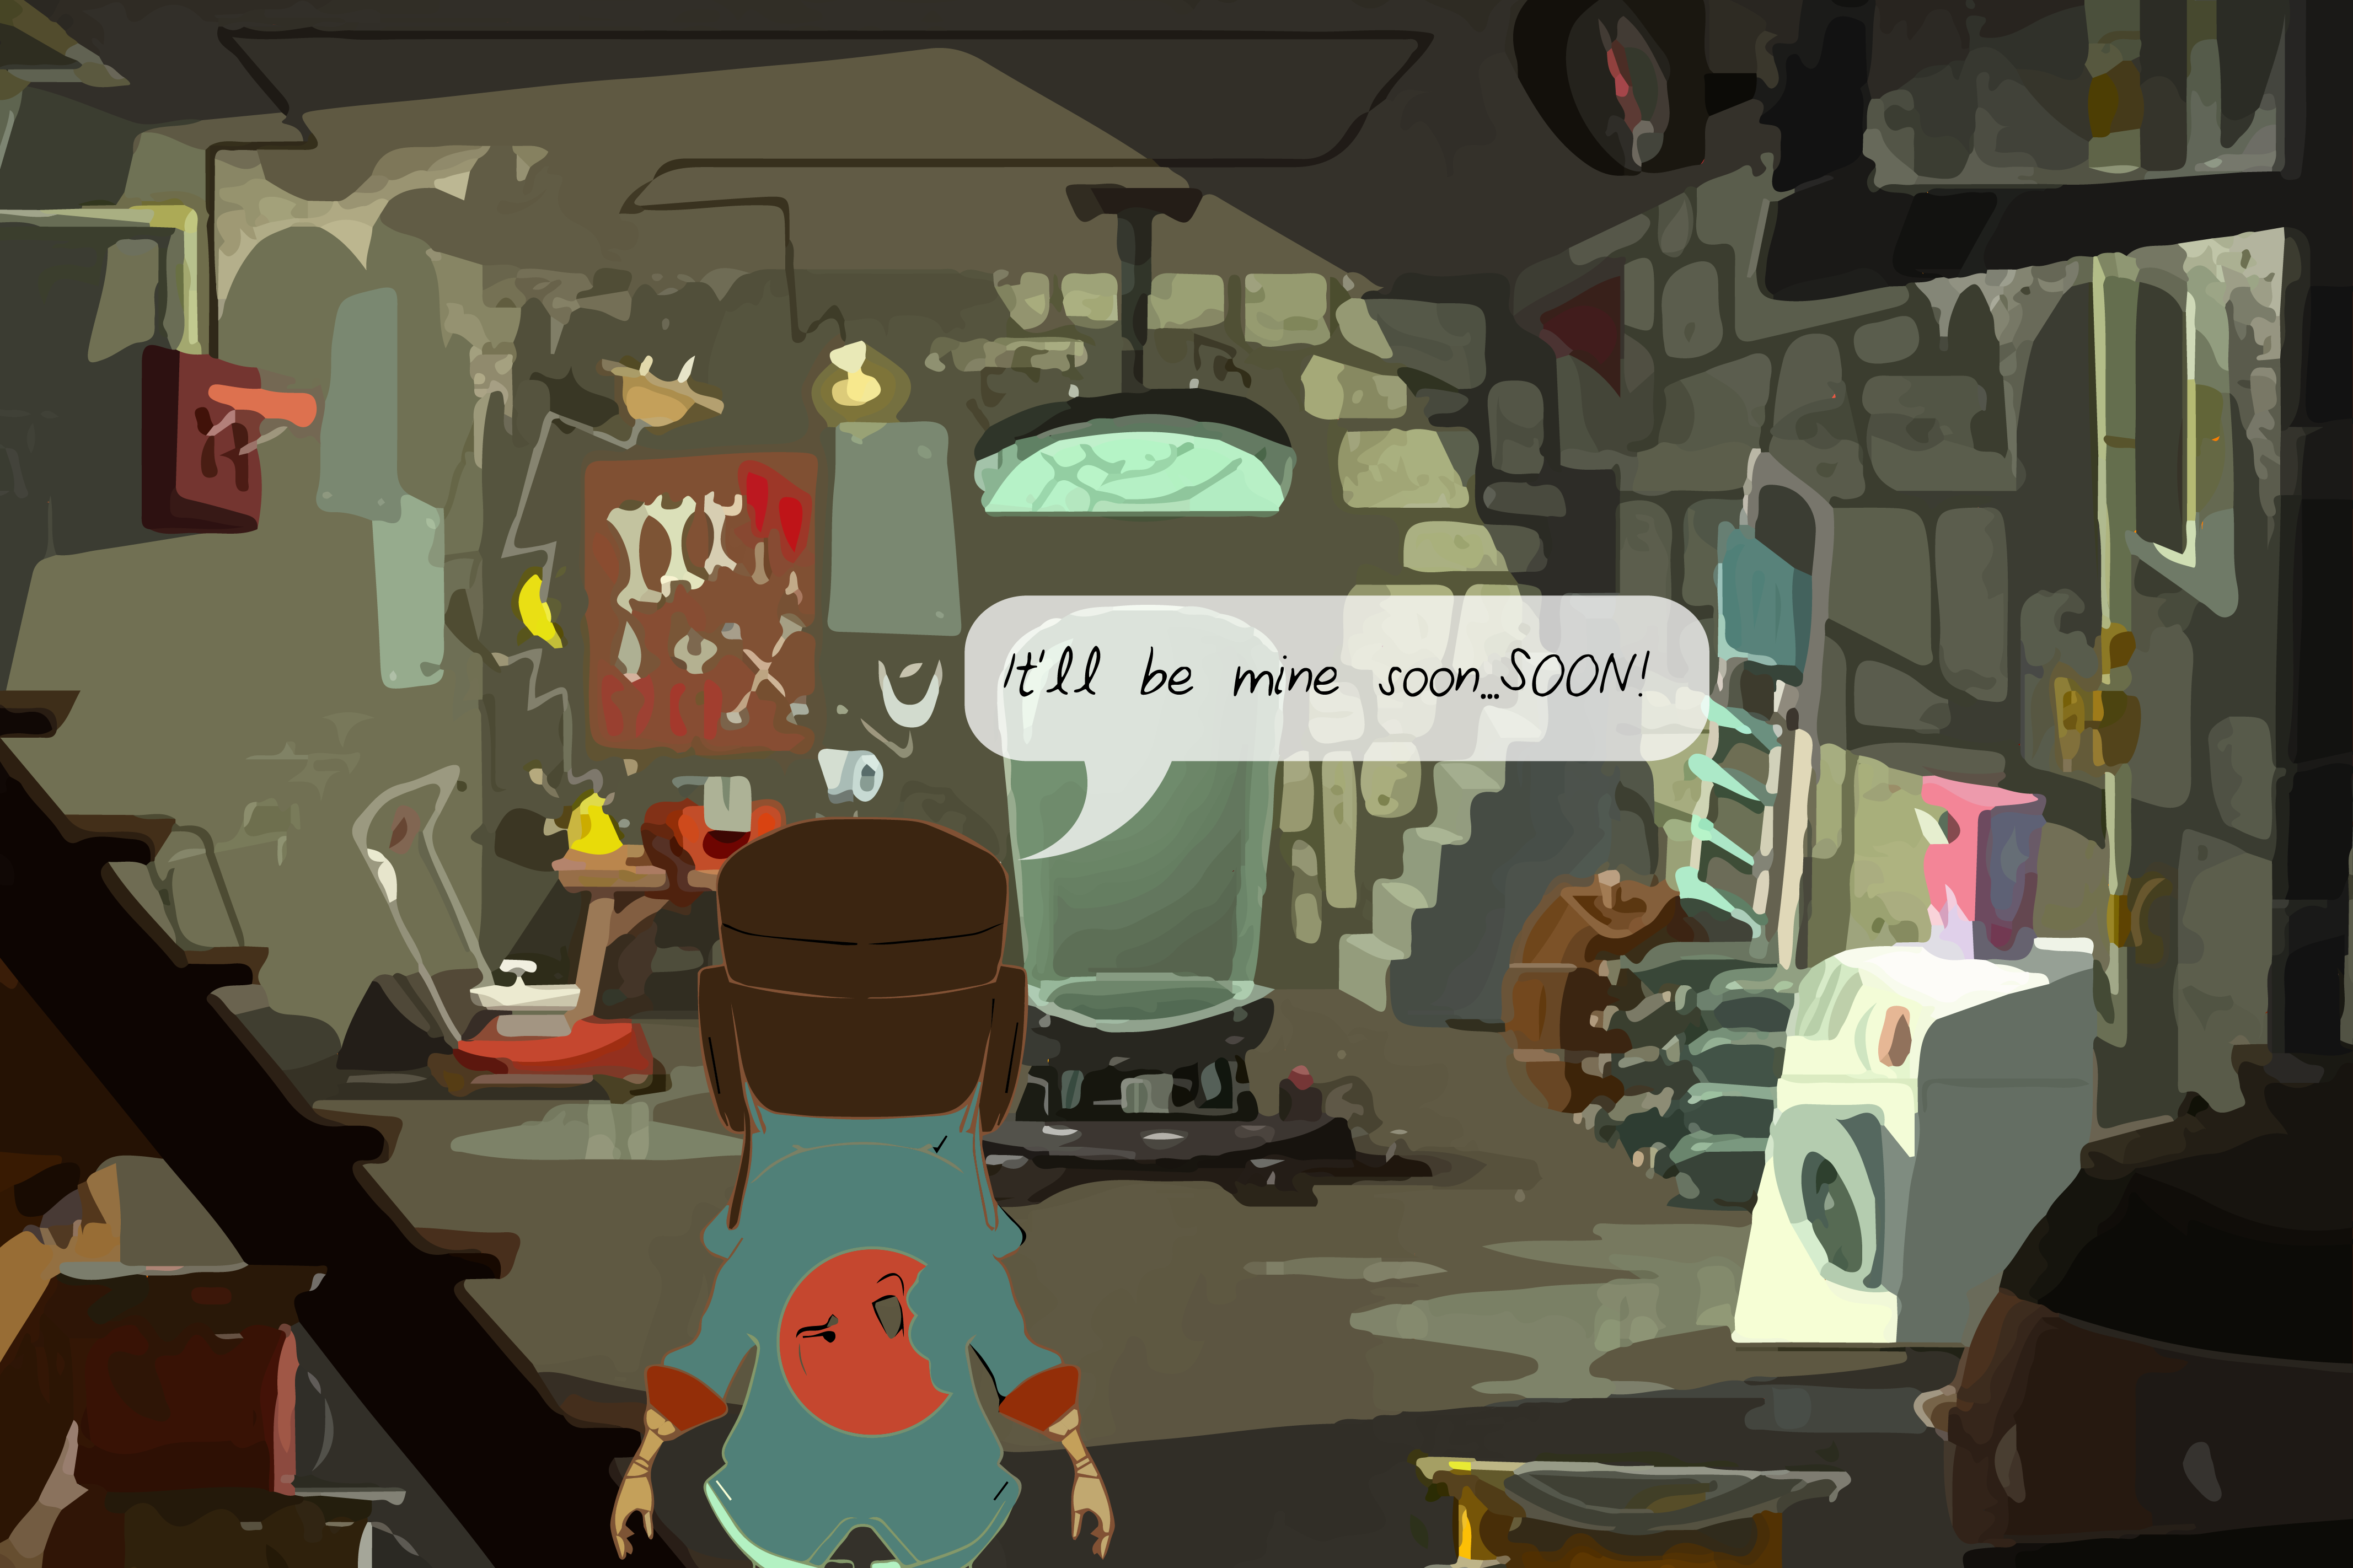
\includegraphics[width=2.3in]{figures/exp1/test-06.png} \\ 
% 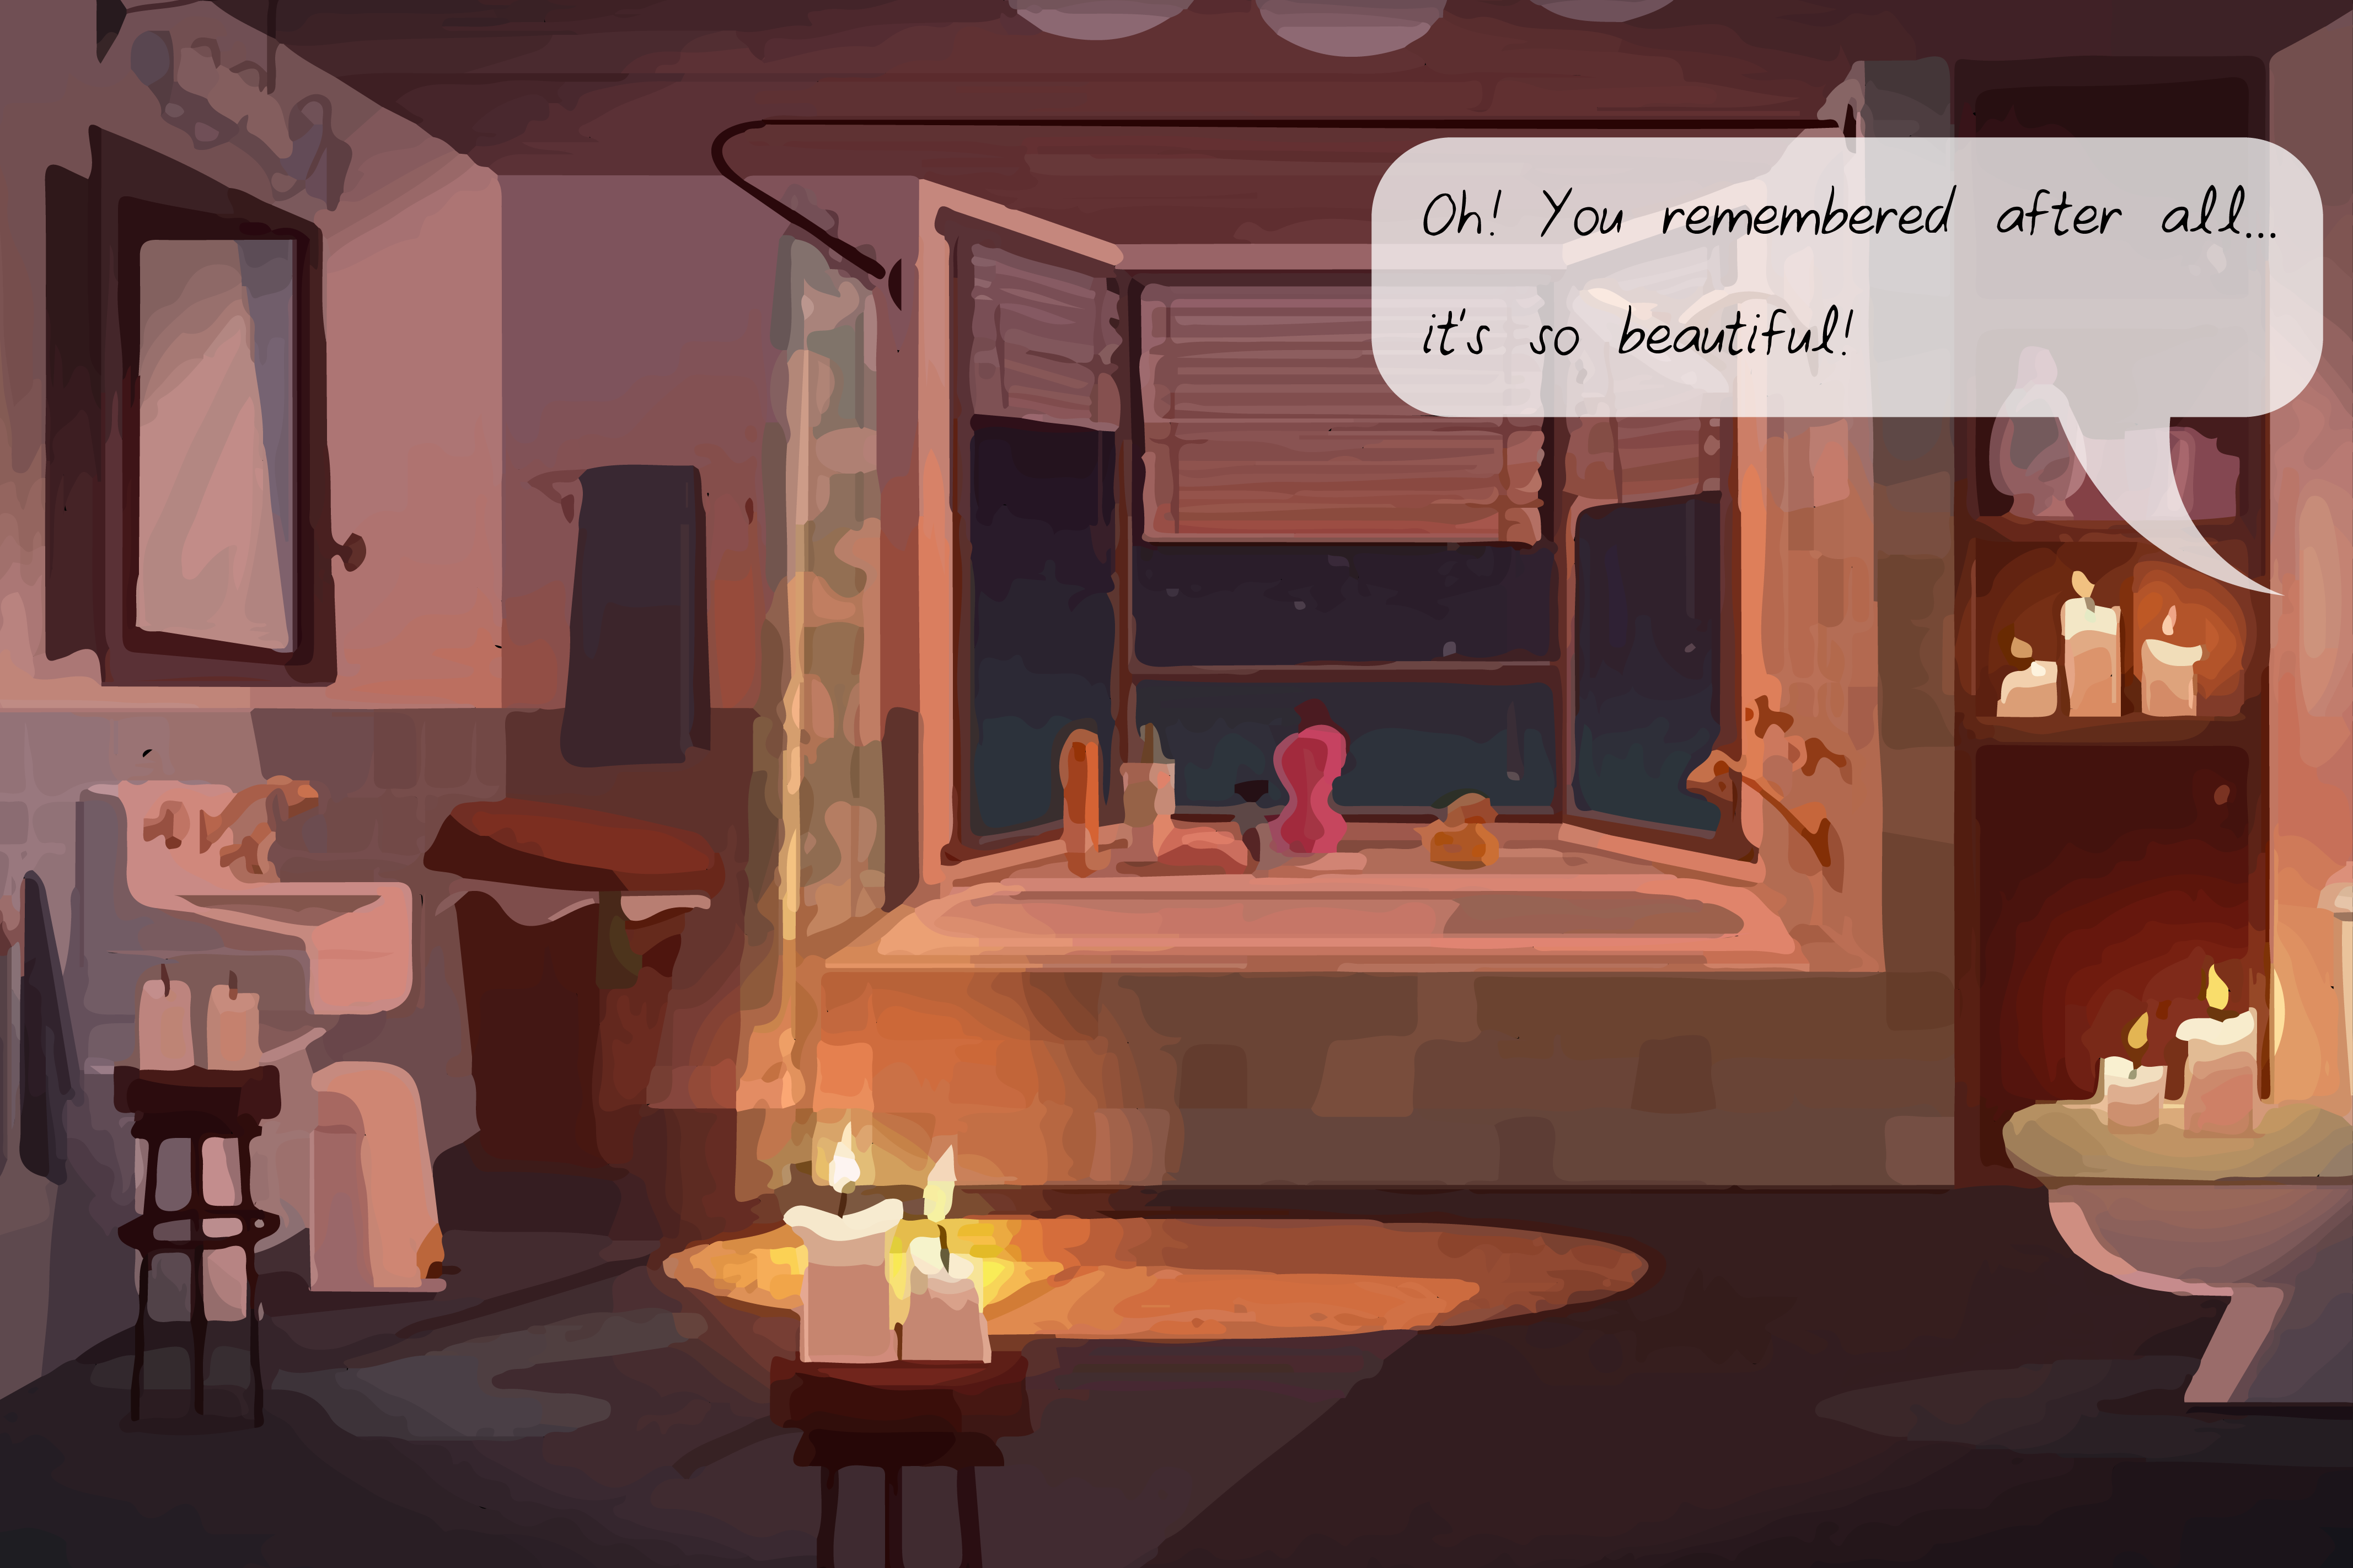
\includegraphics[width=2.3in]{figures/exp1/test-07.png} &
% 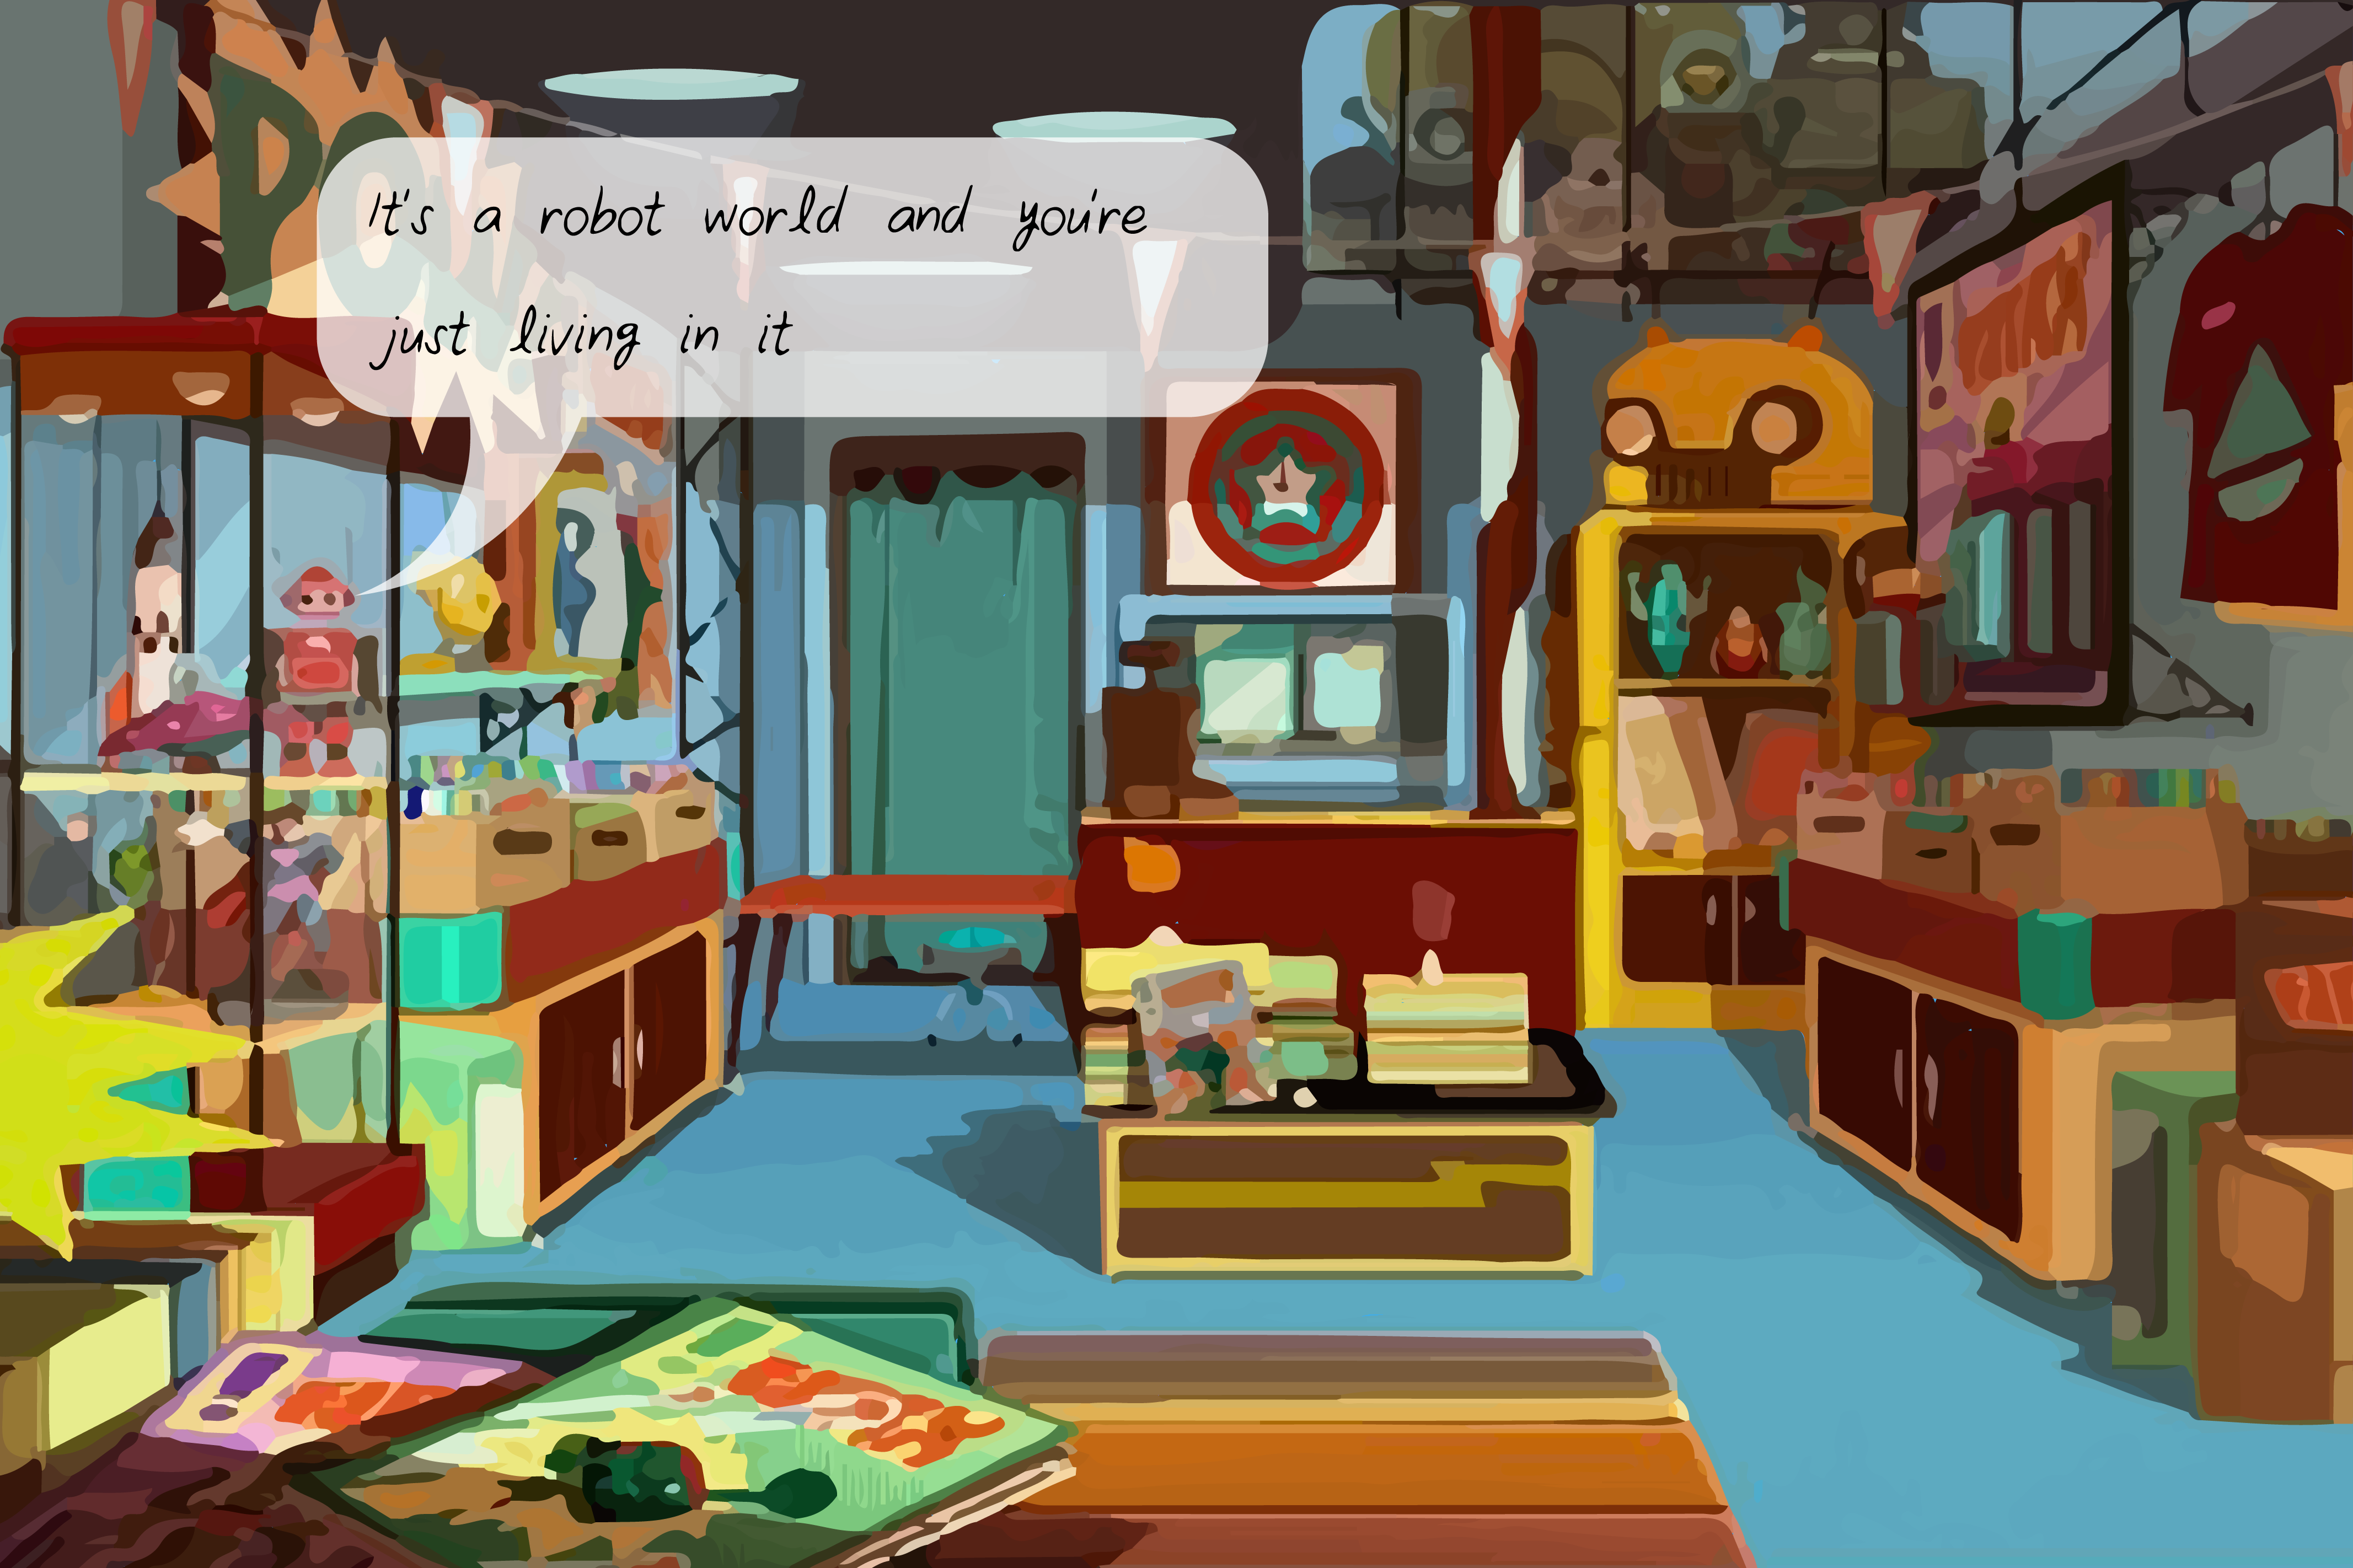
\includegraphics[width=2.3in]{figures/exp1/test-08.png} \\ 
% 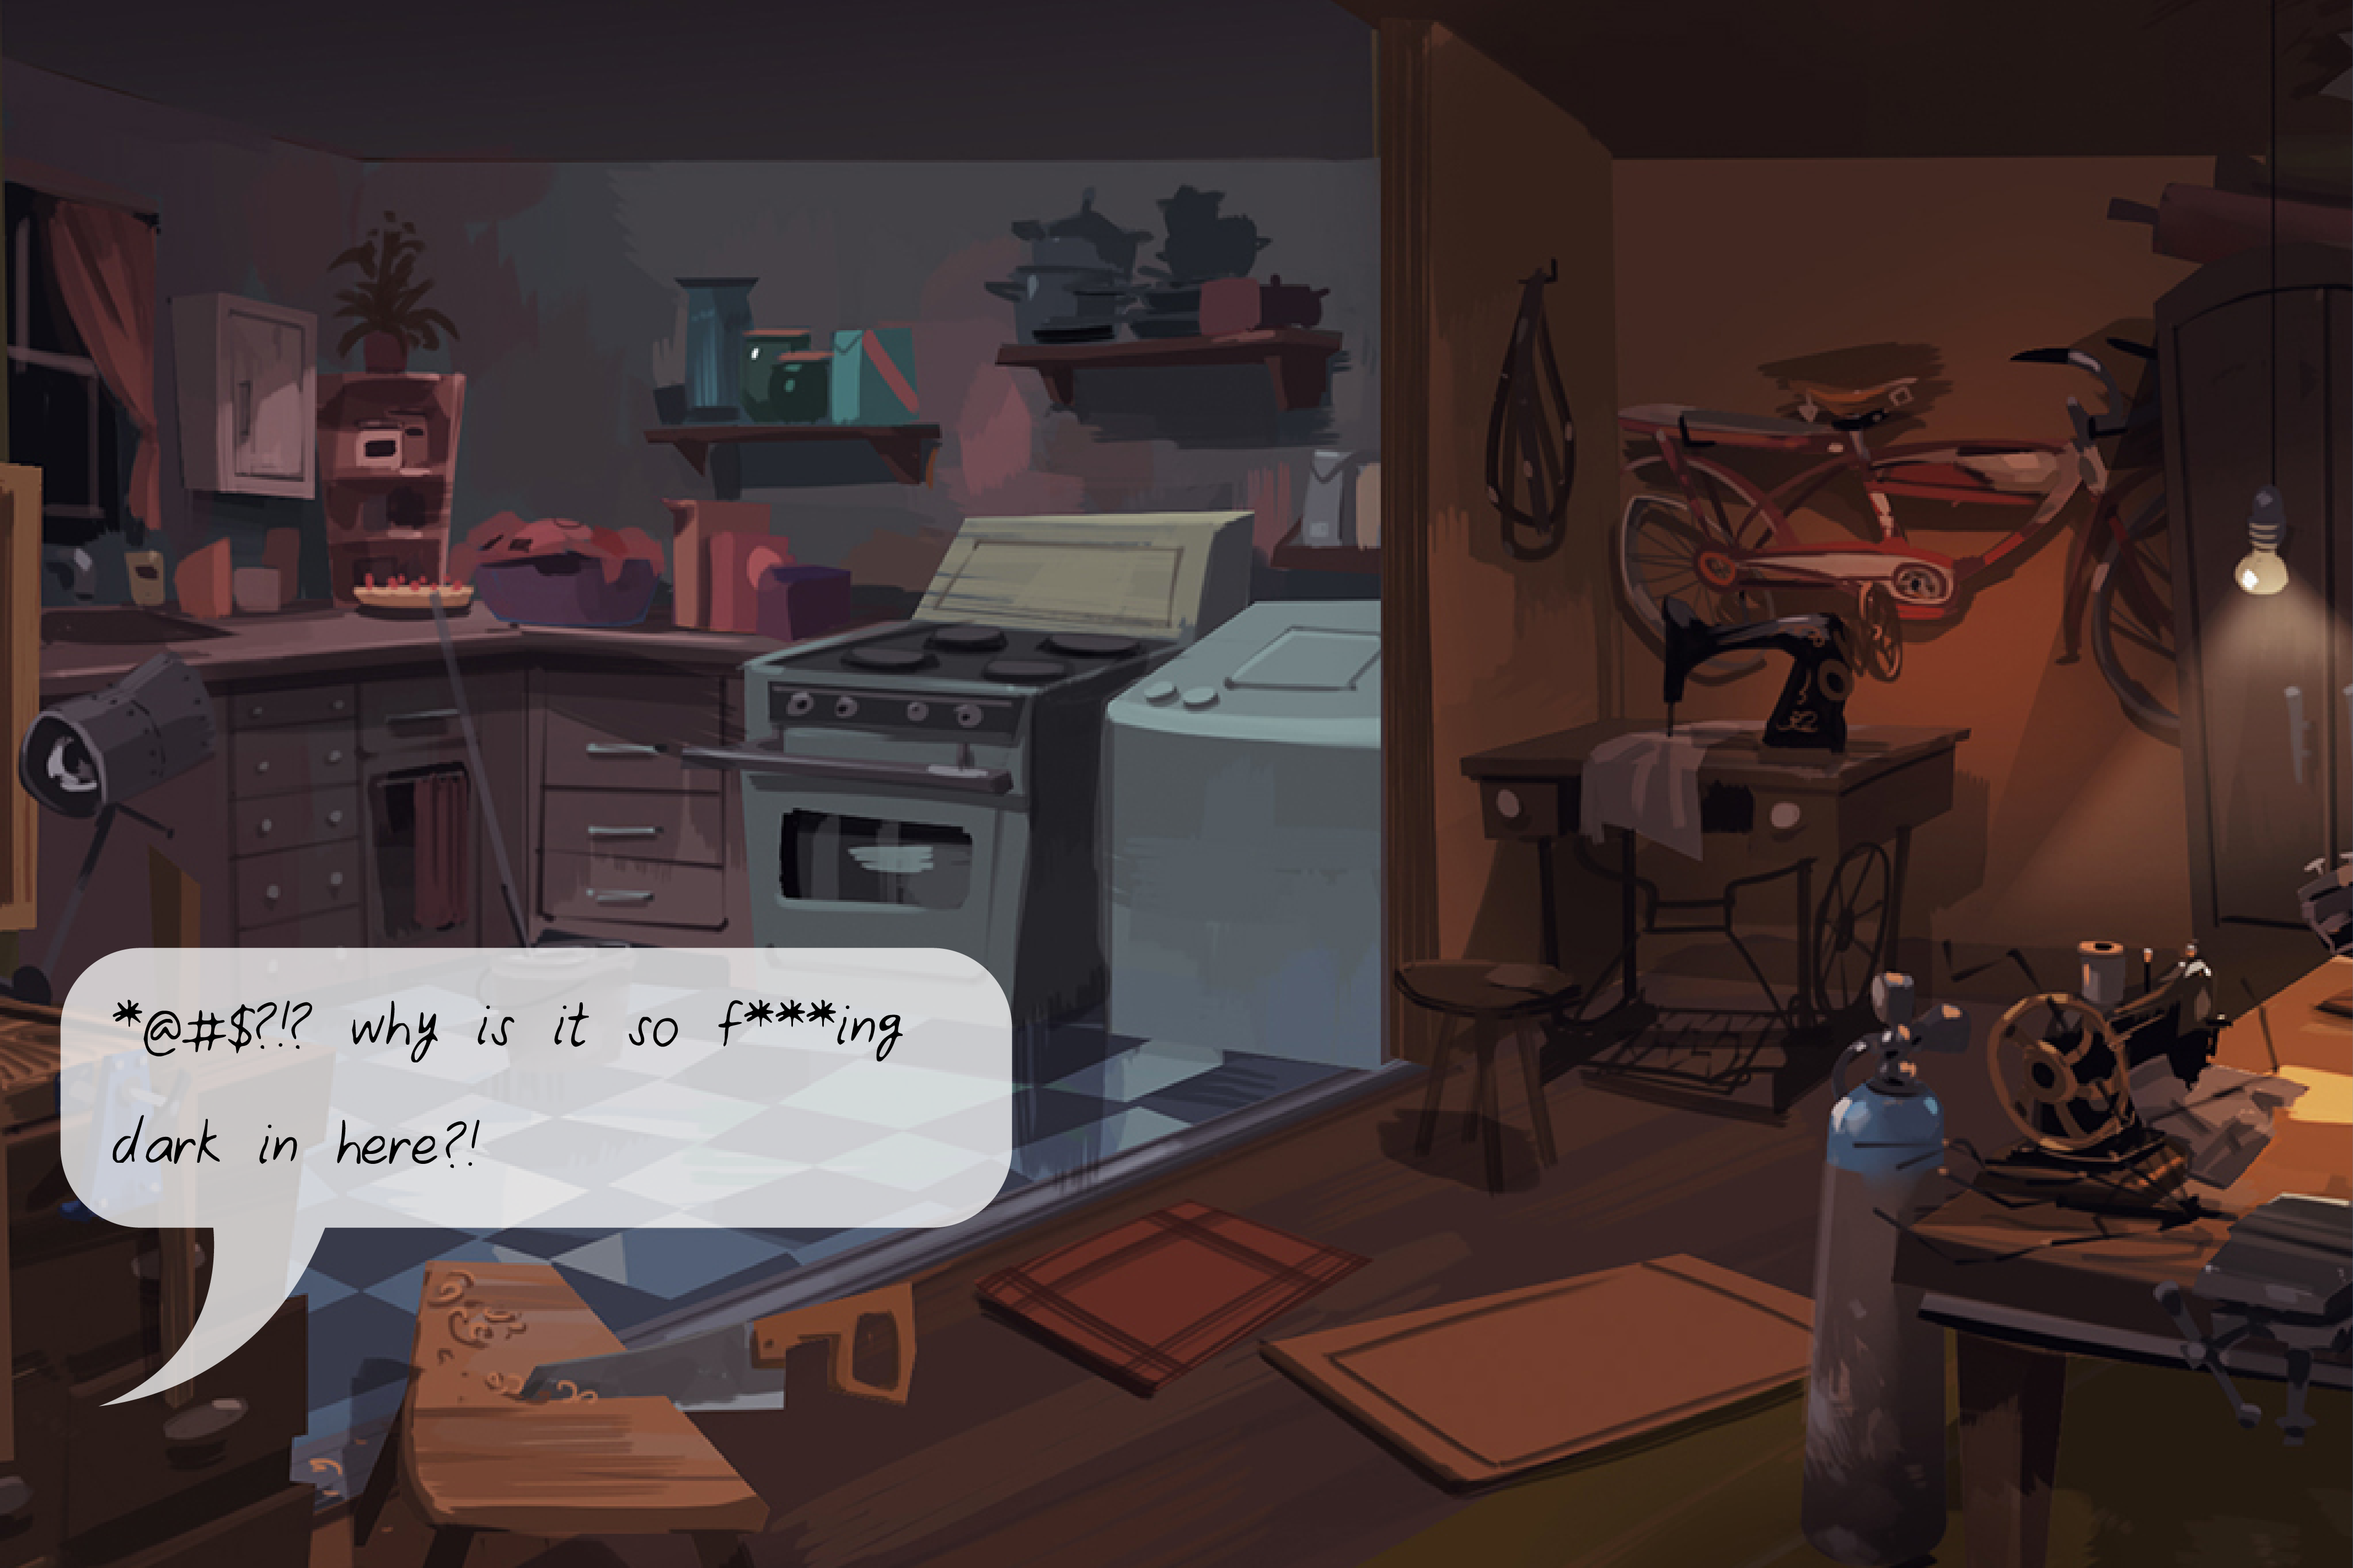
\includegraphics[width=2.3in]{figures/exp1/test-09.png} &
% 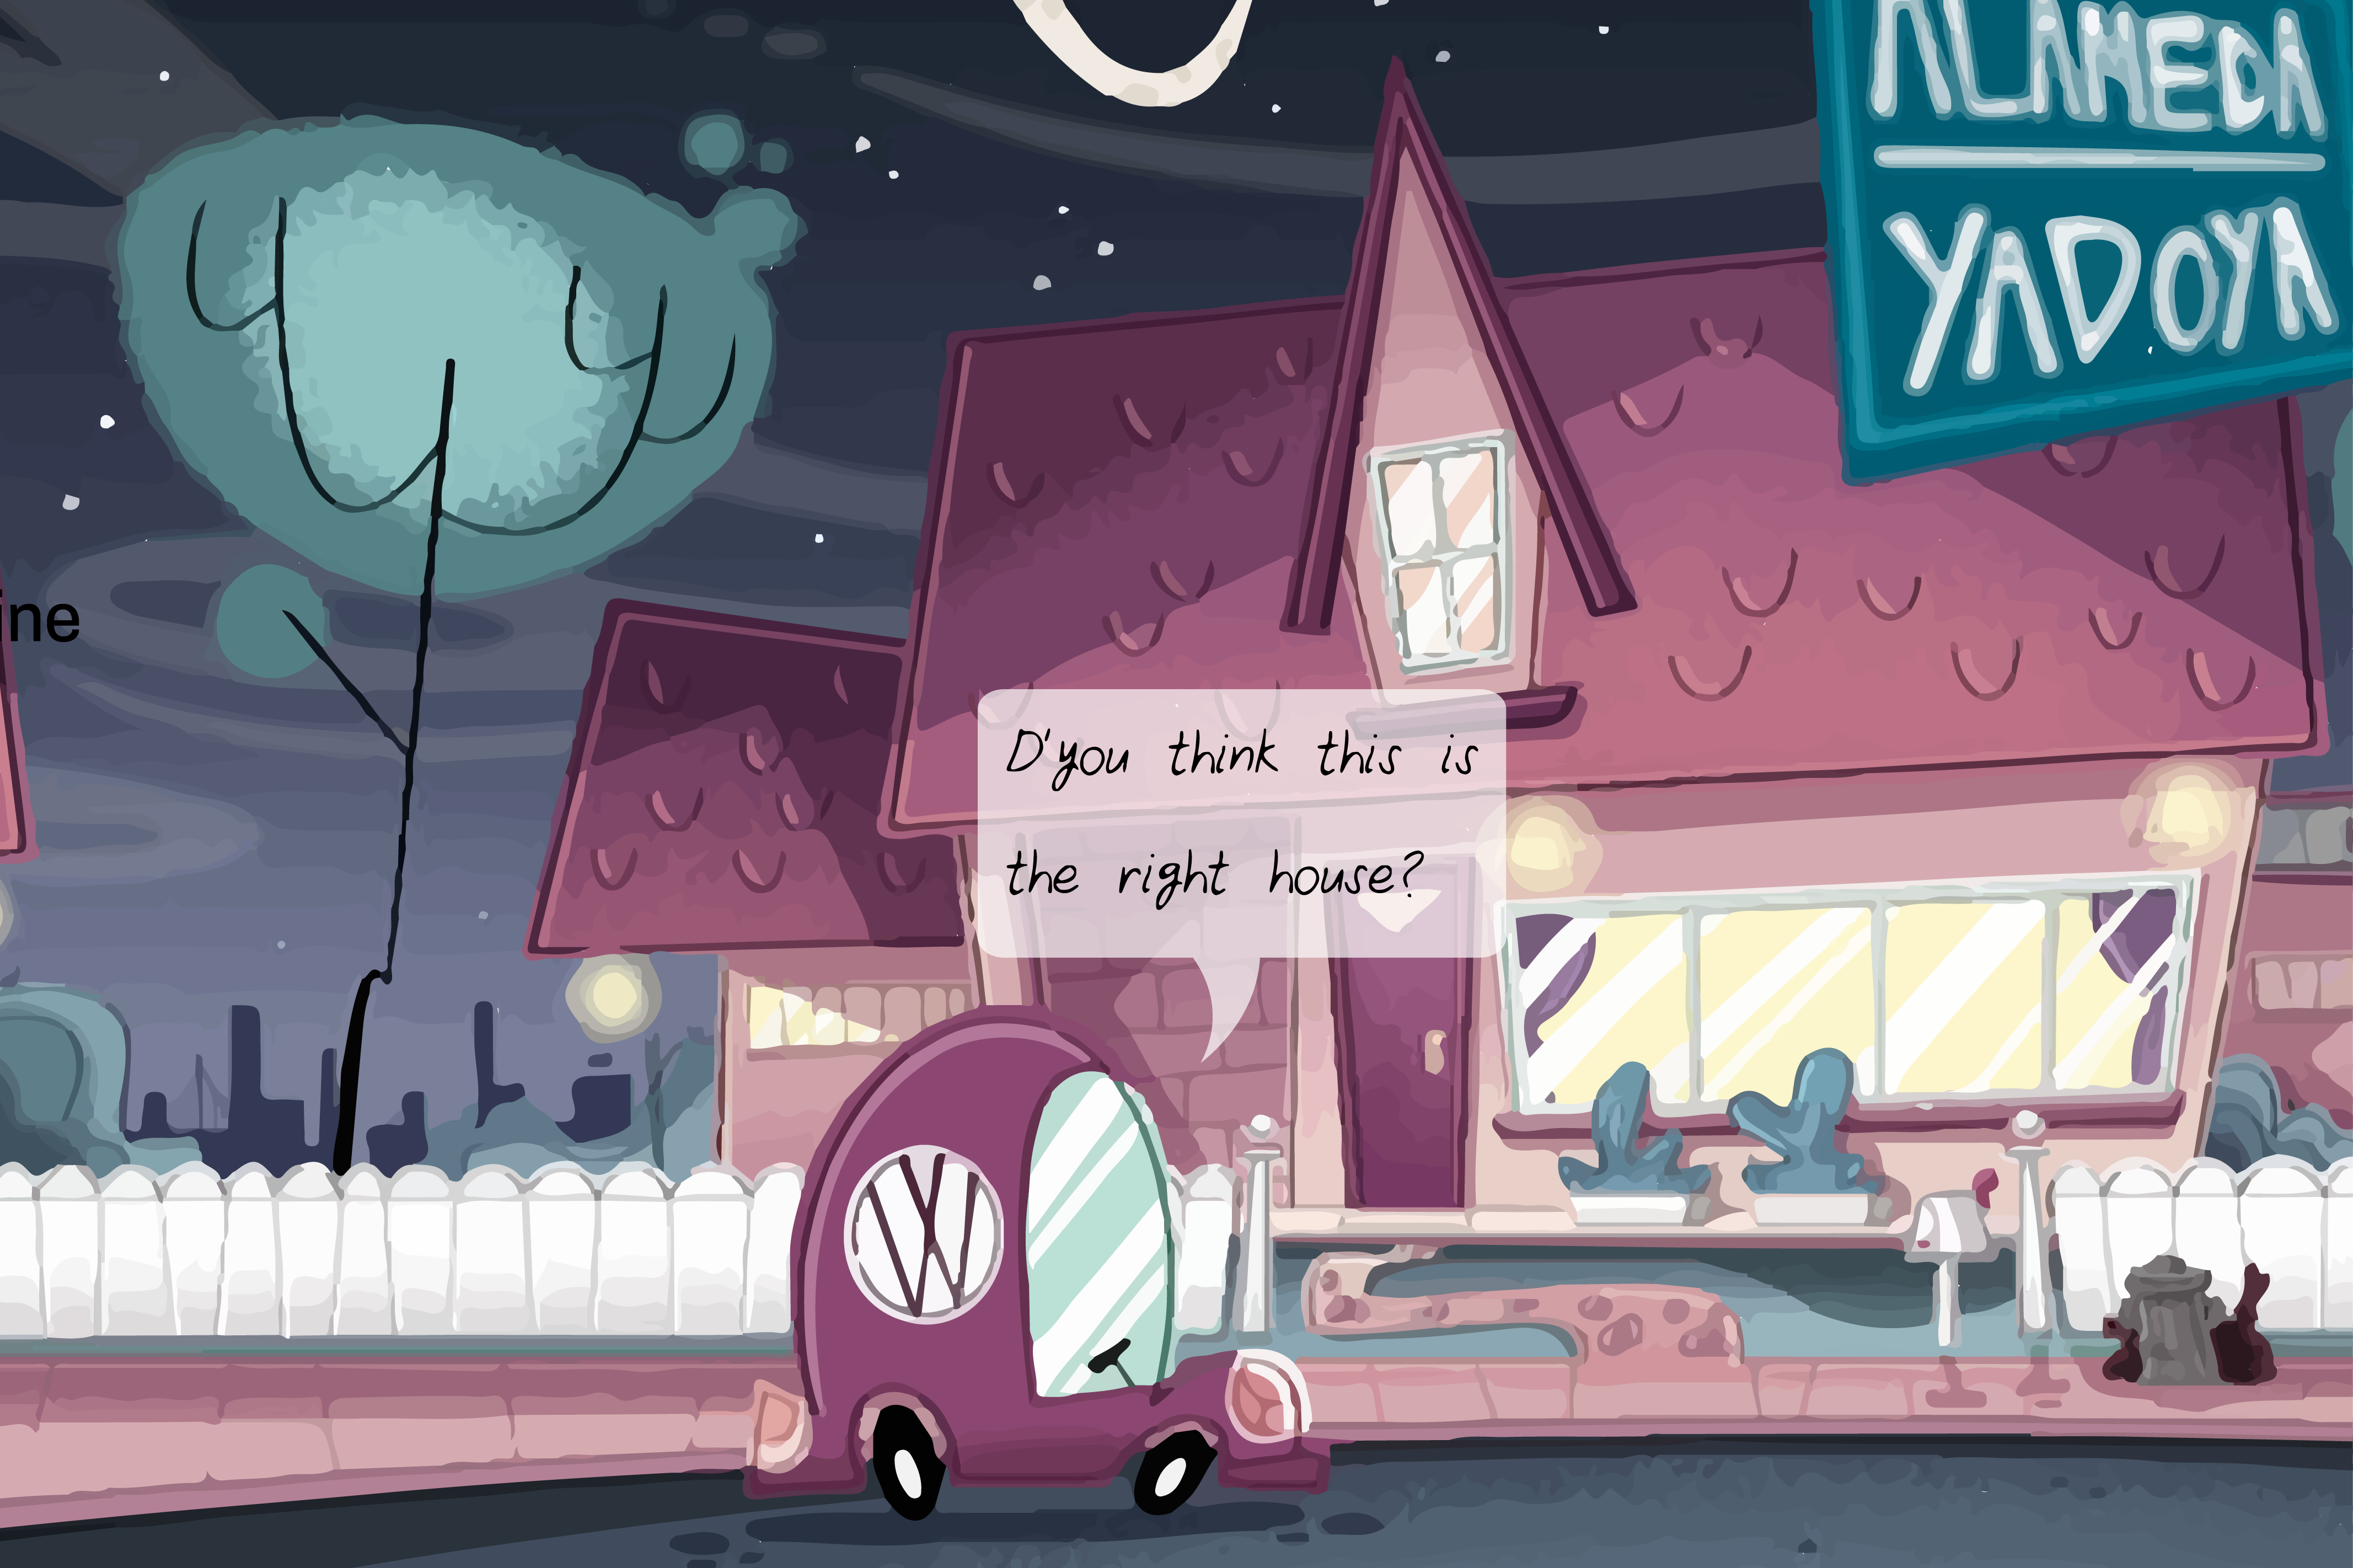
\includegraphics[width=2.3in]{figures/exp1/test-10.png}
% \end{array}$
% \end{center}
% \end{figure}

% \begin{figure}[h]
% \begin{center}$
% \begin{array}{c c}
% 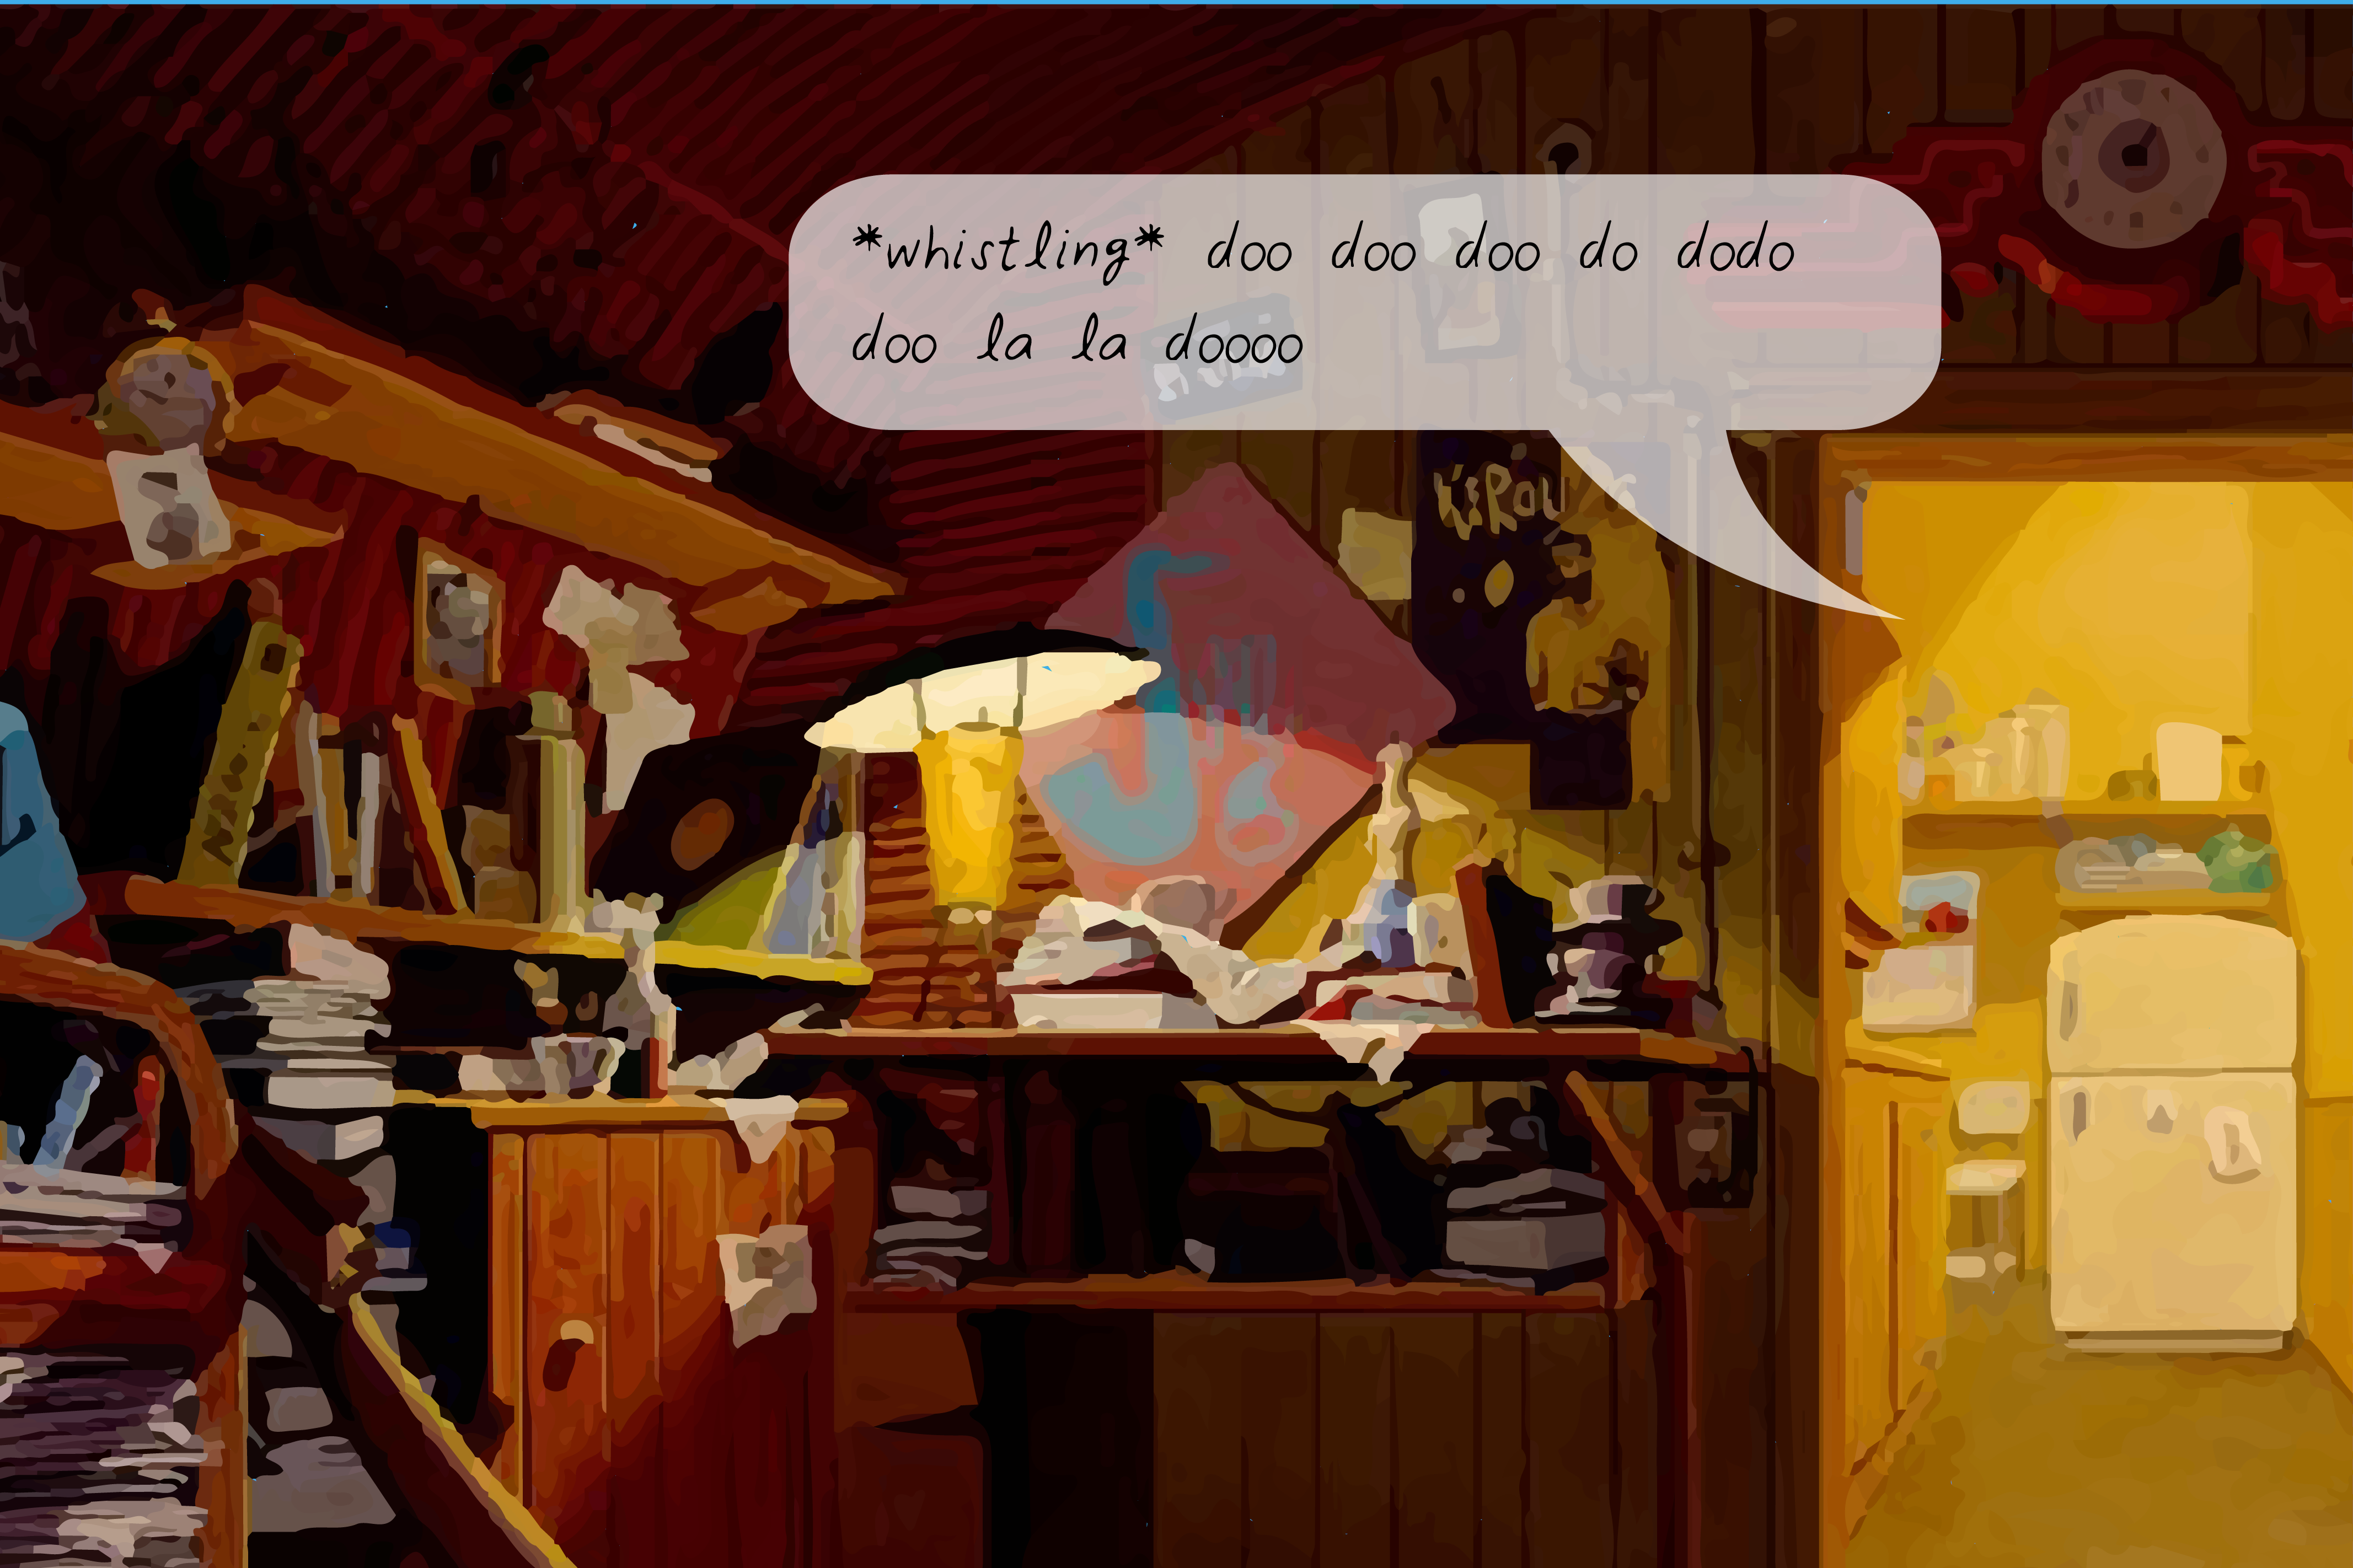
\includegraphics[width=2.5in]{figures/exp1/test-11.png} &
% 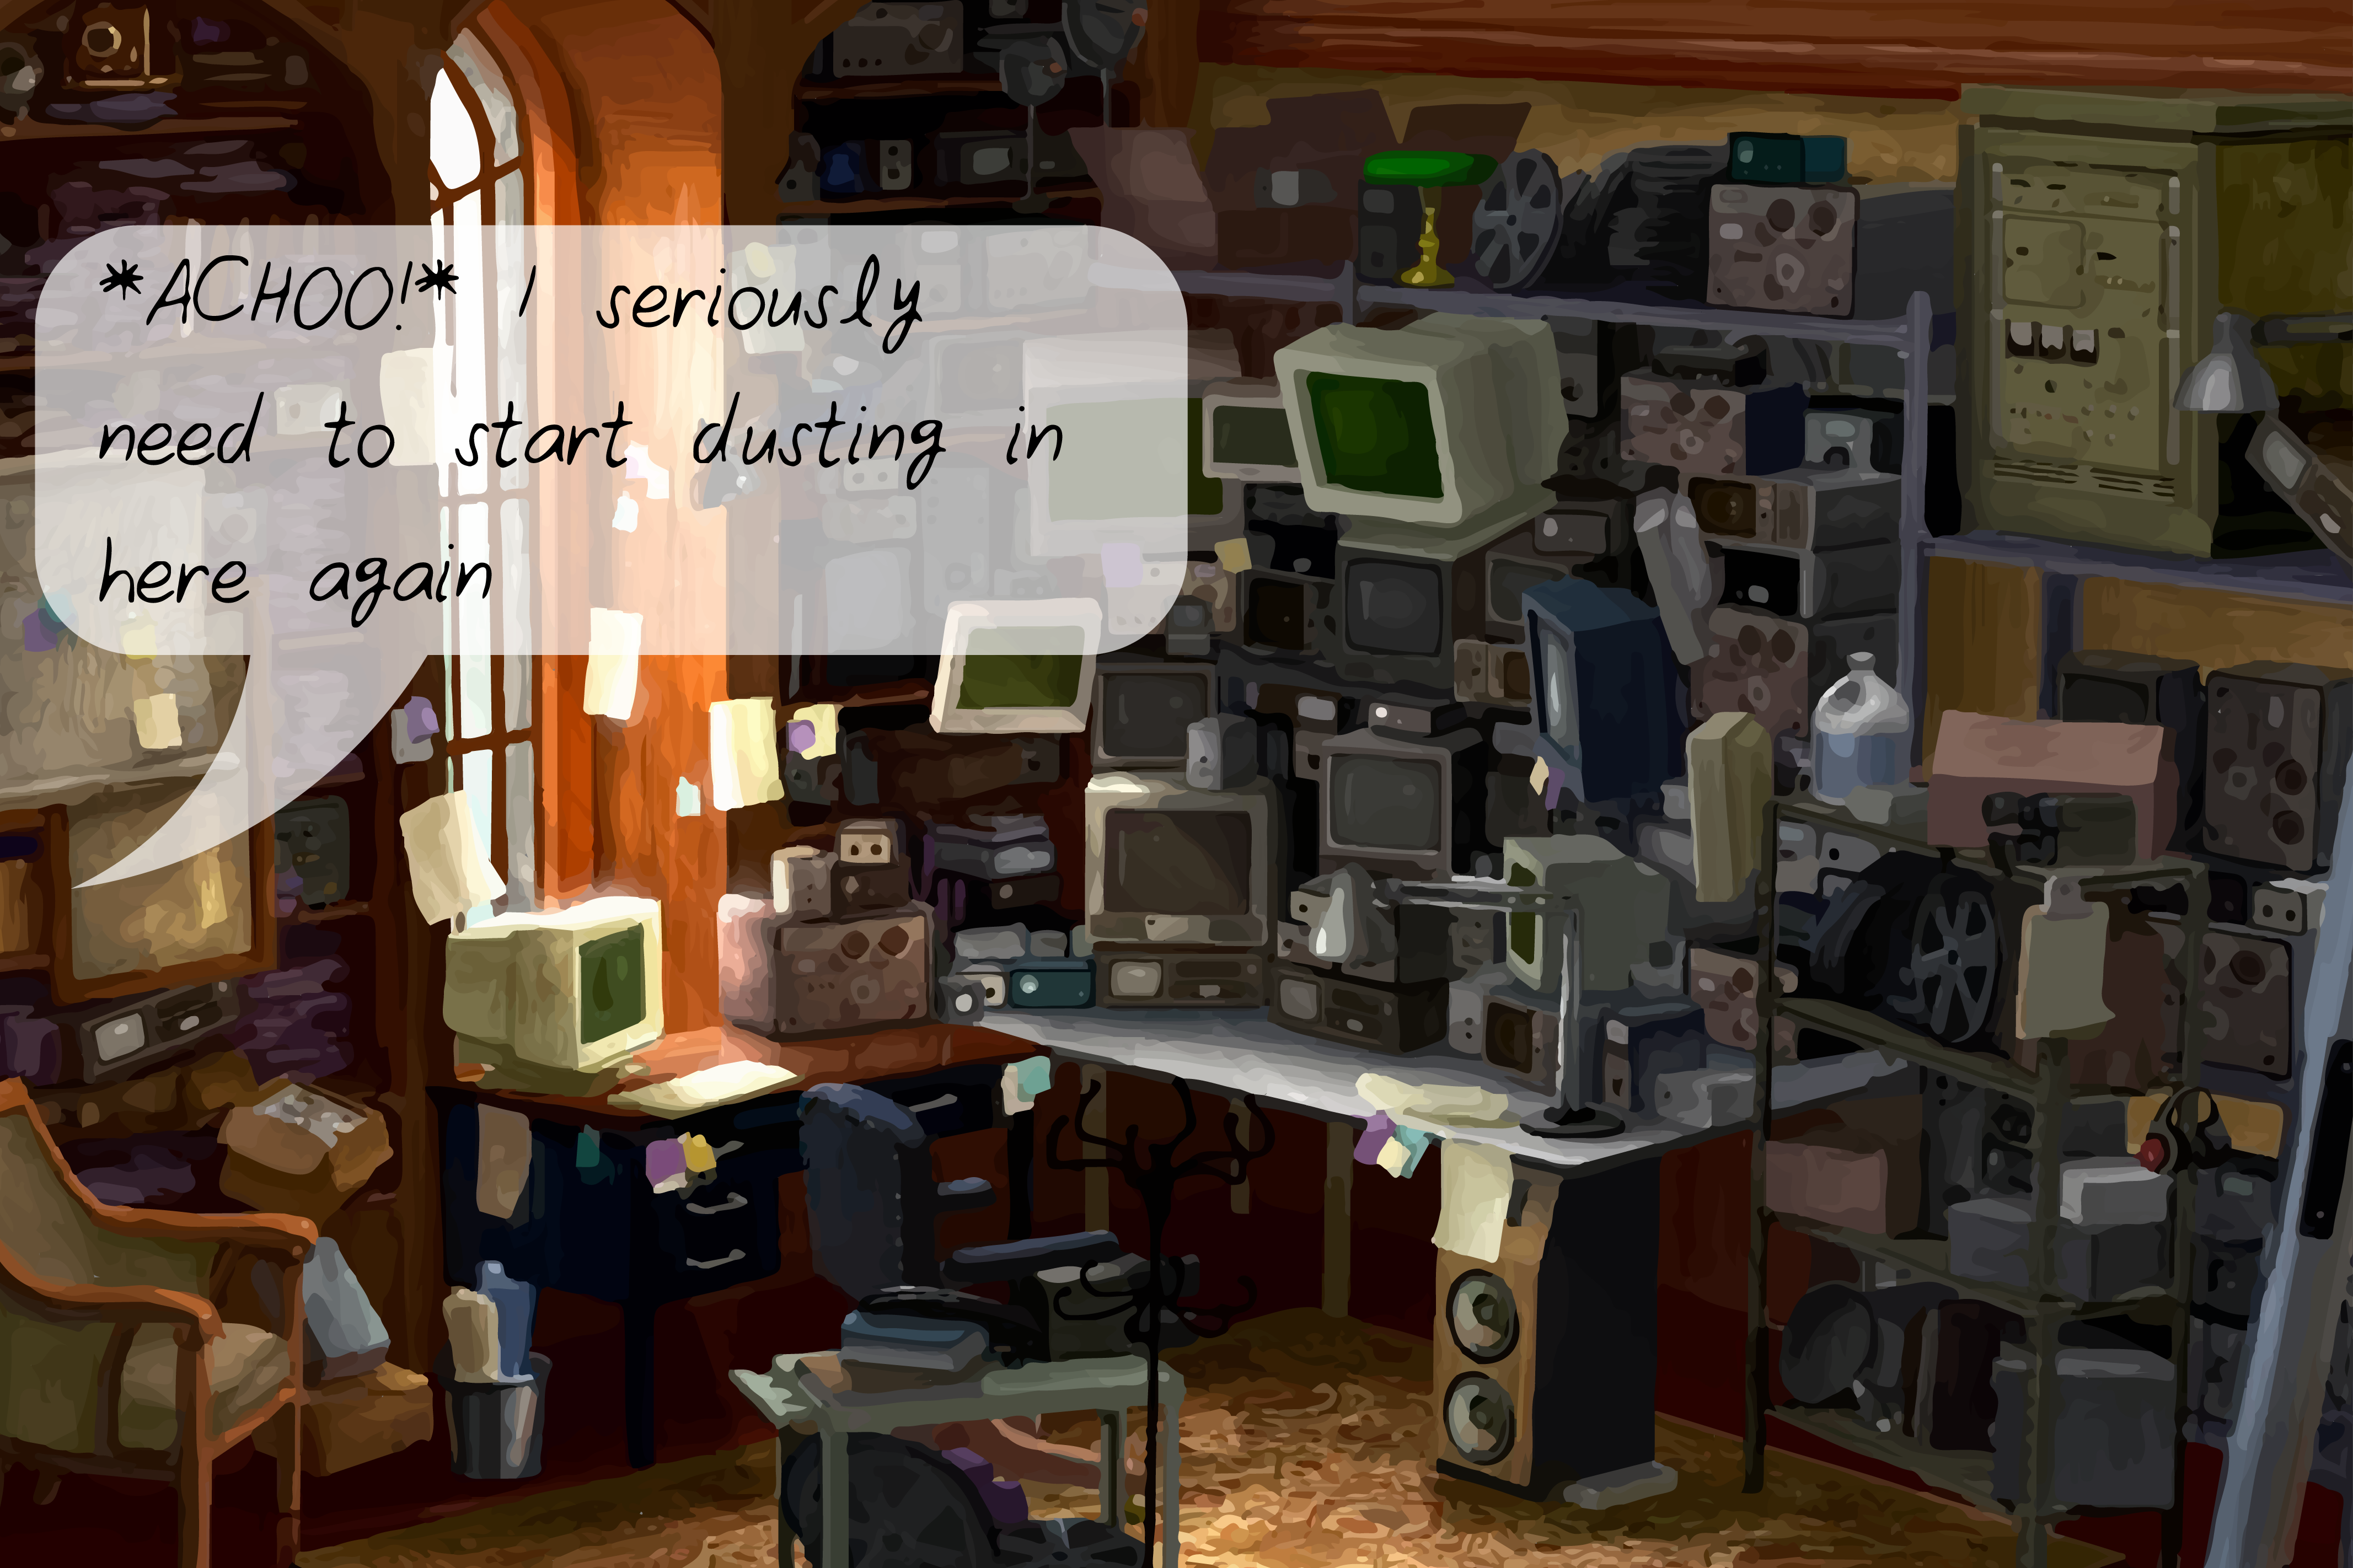
\includegraphics[width=2.5in]{figures/exp1/test-12.png} \\ 
% 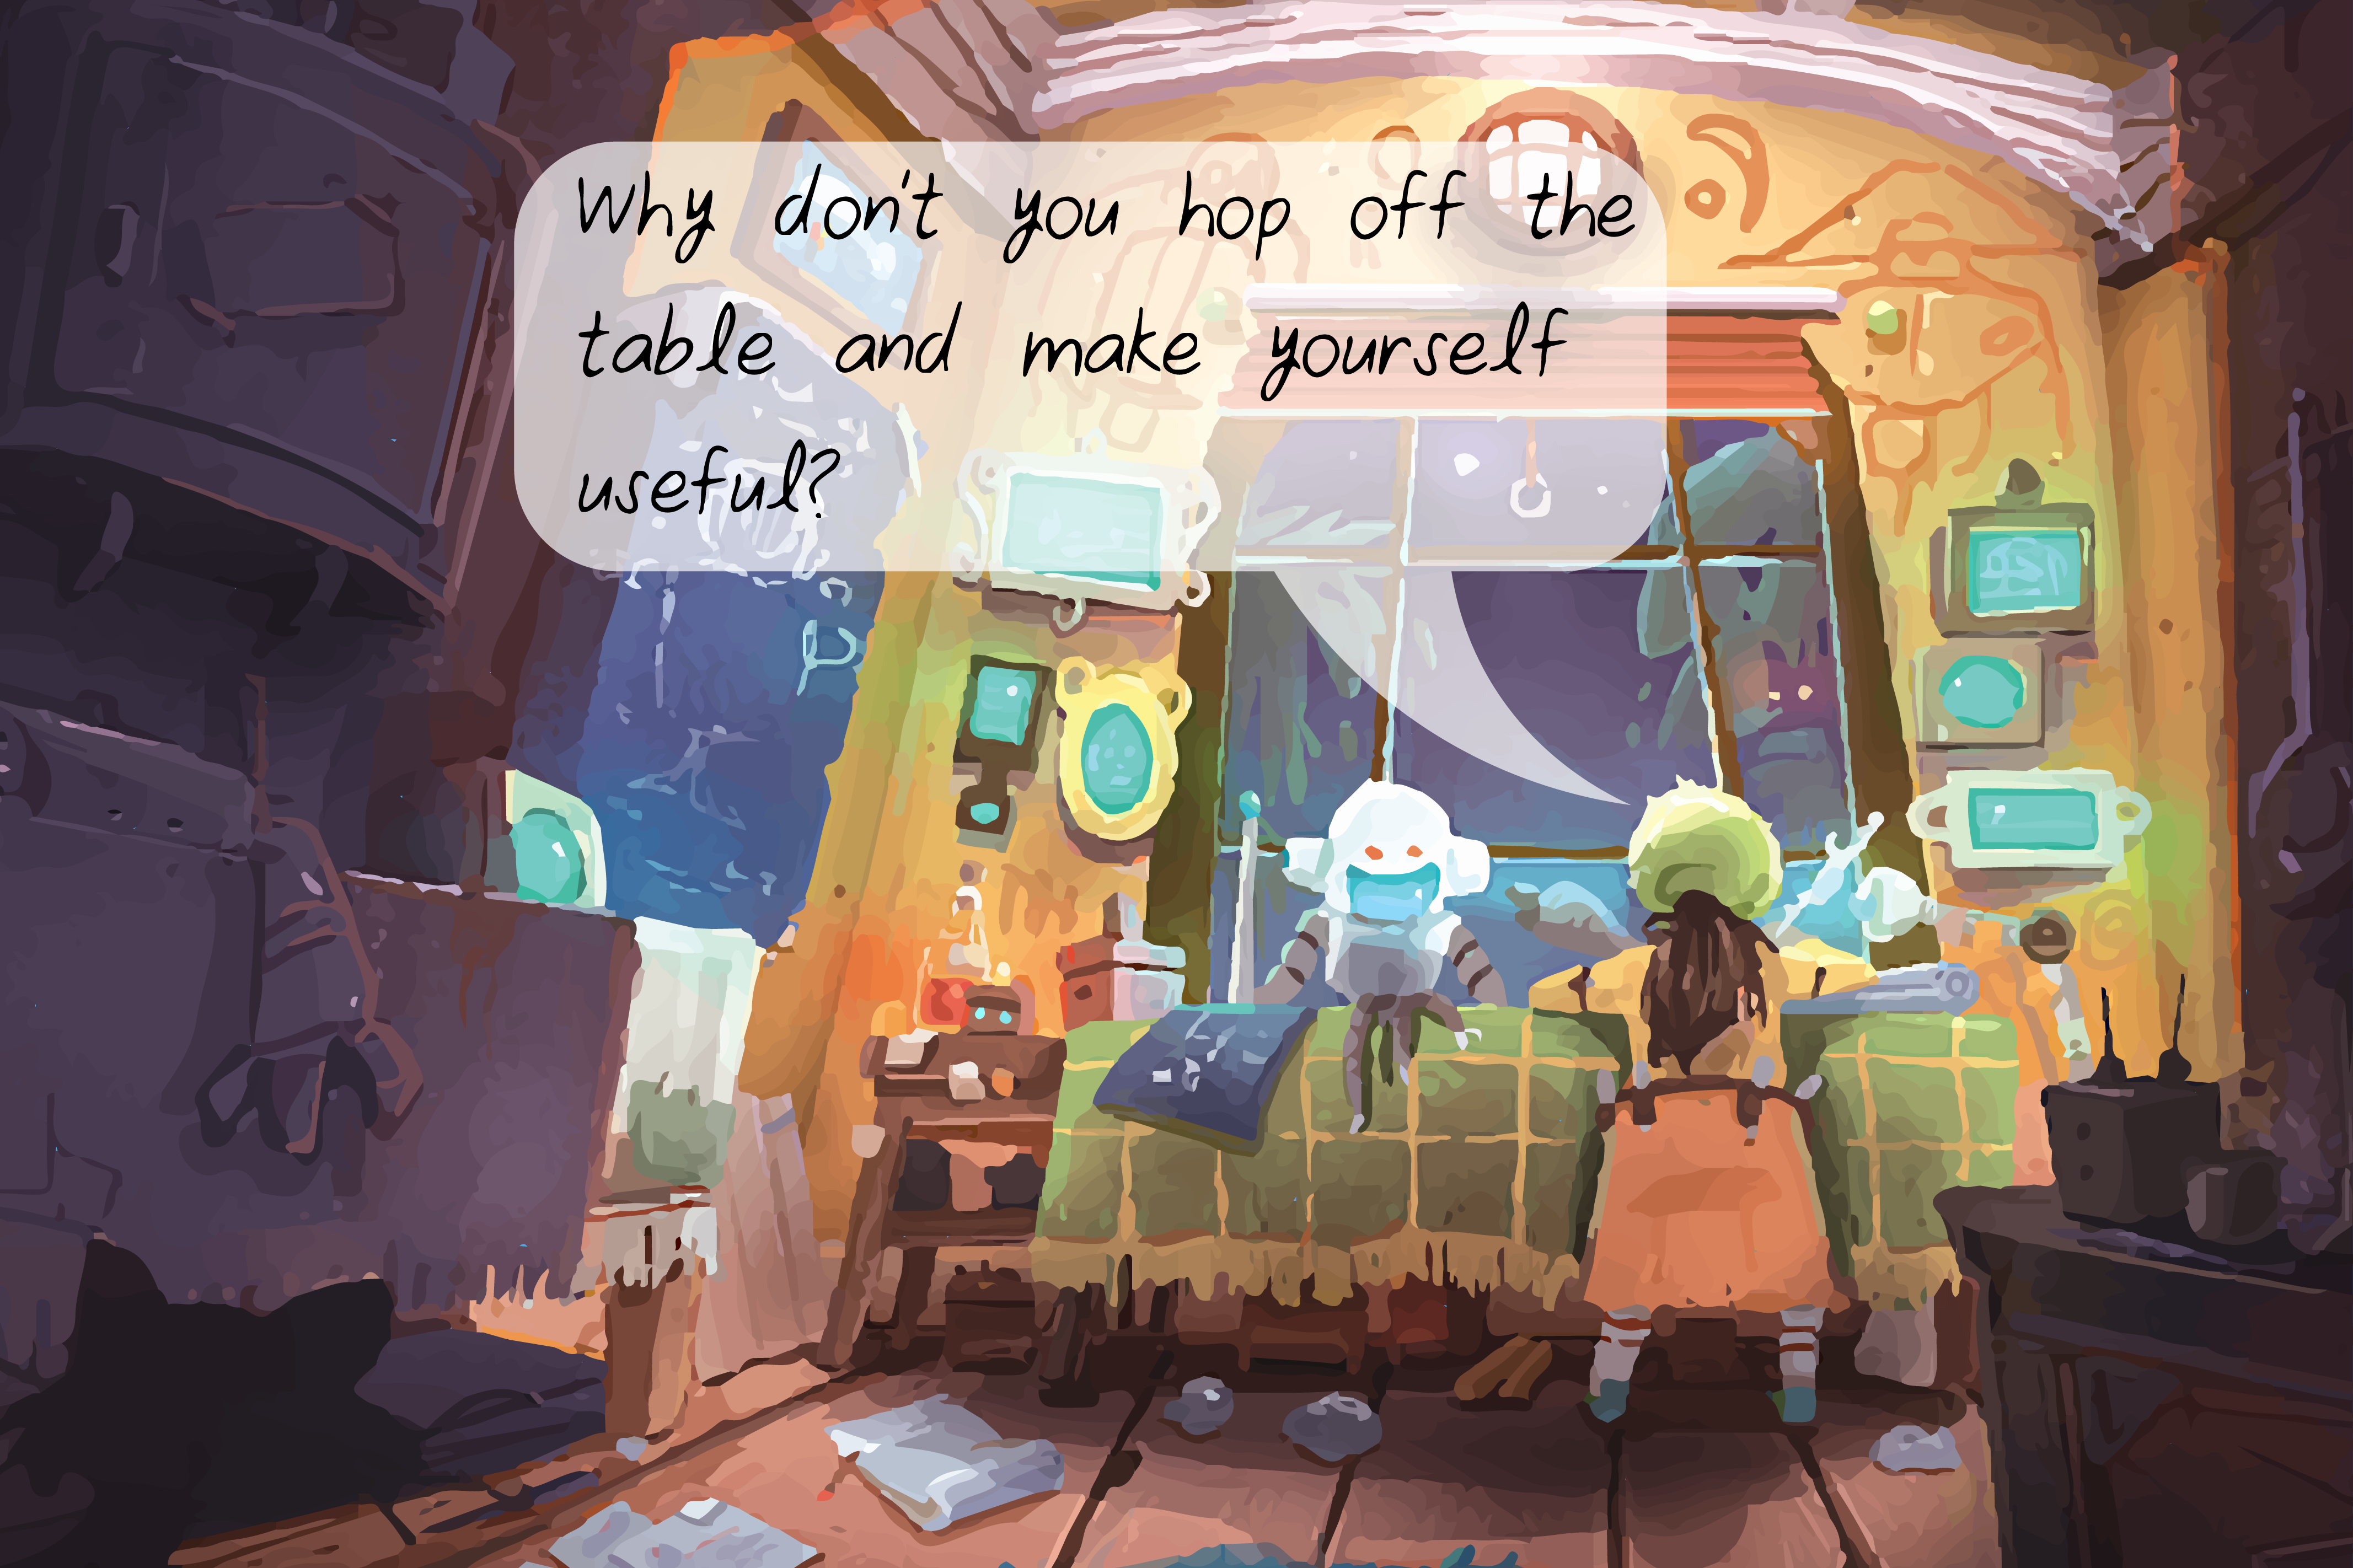
\includegraphics[width=2.5in]{figures/exp1/test-13.png} &
% 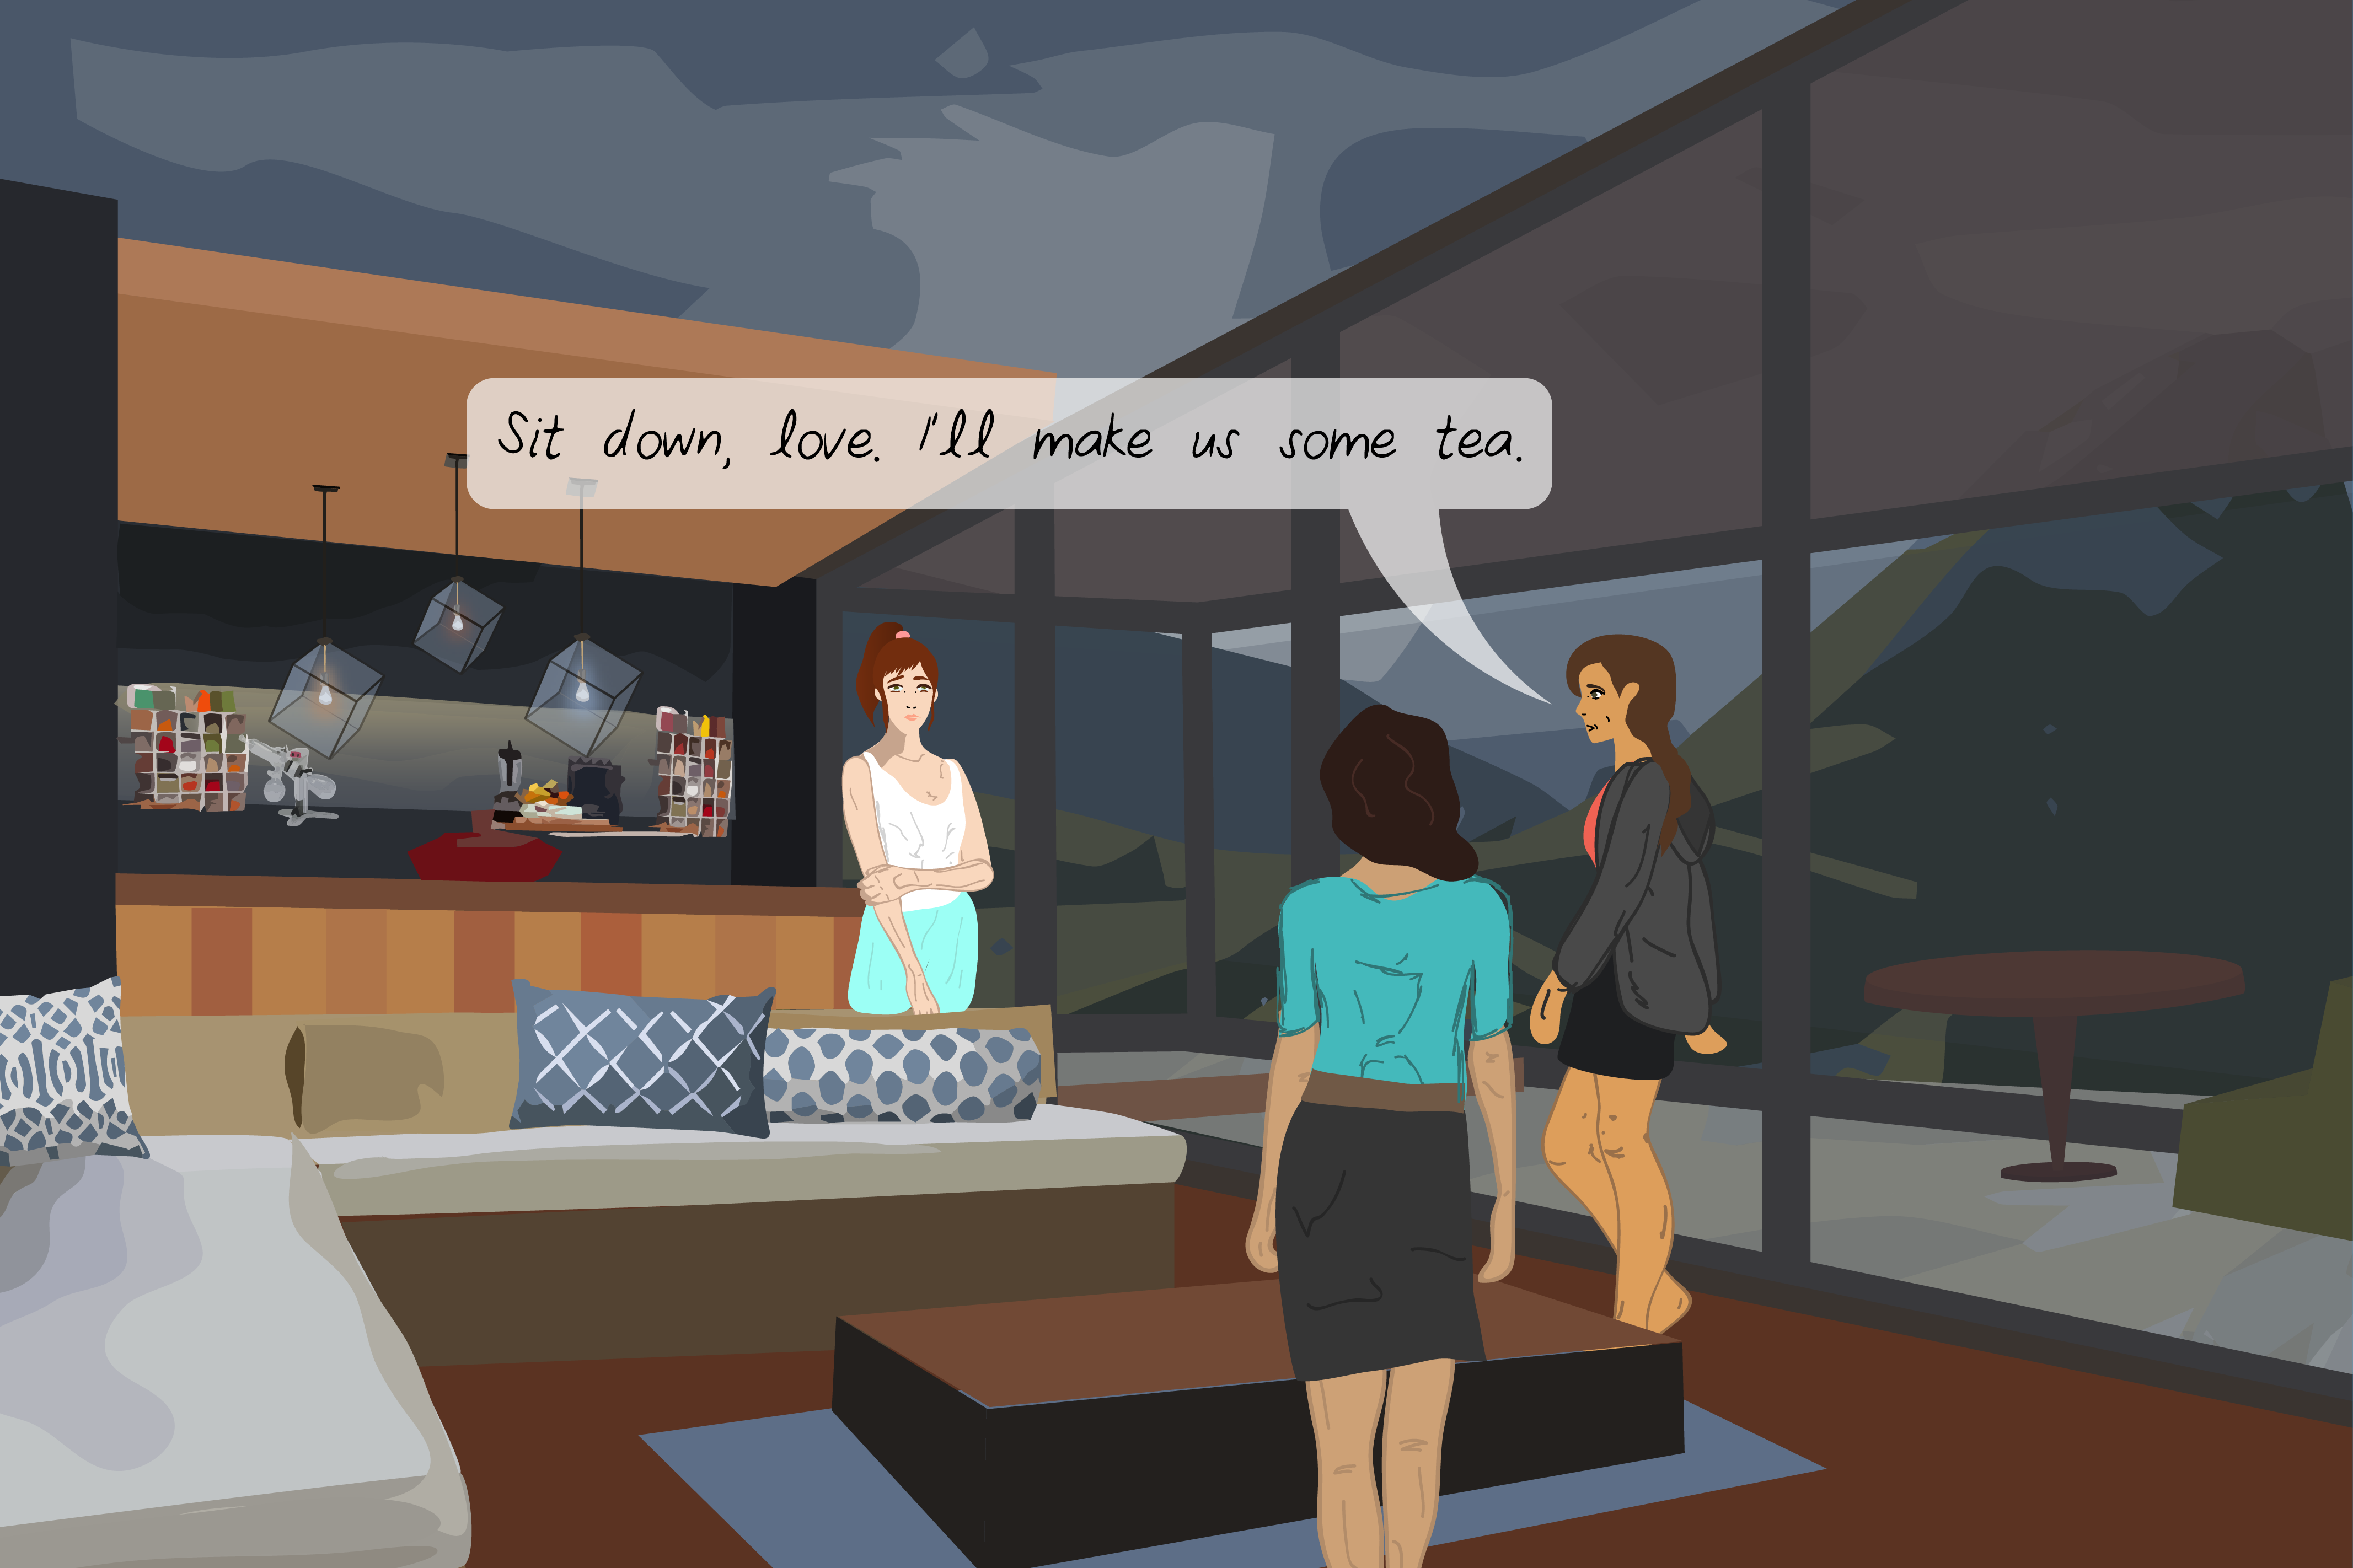
\includegraphics[width=2.5in]{figures/exp1/test-14.png} \\ 
% 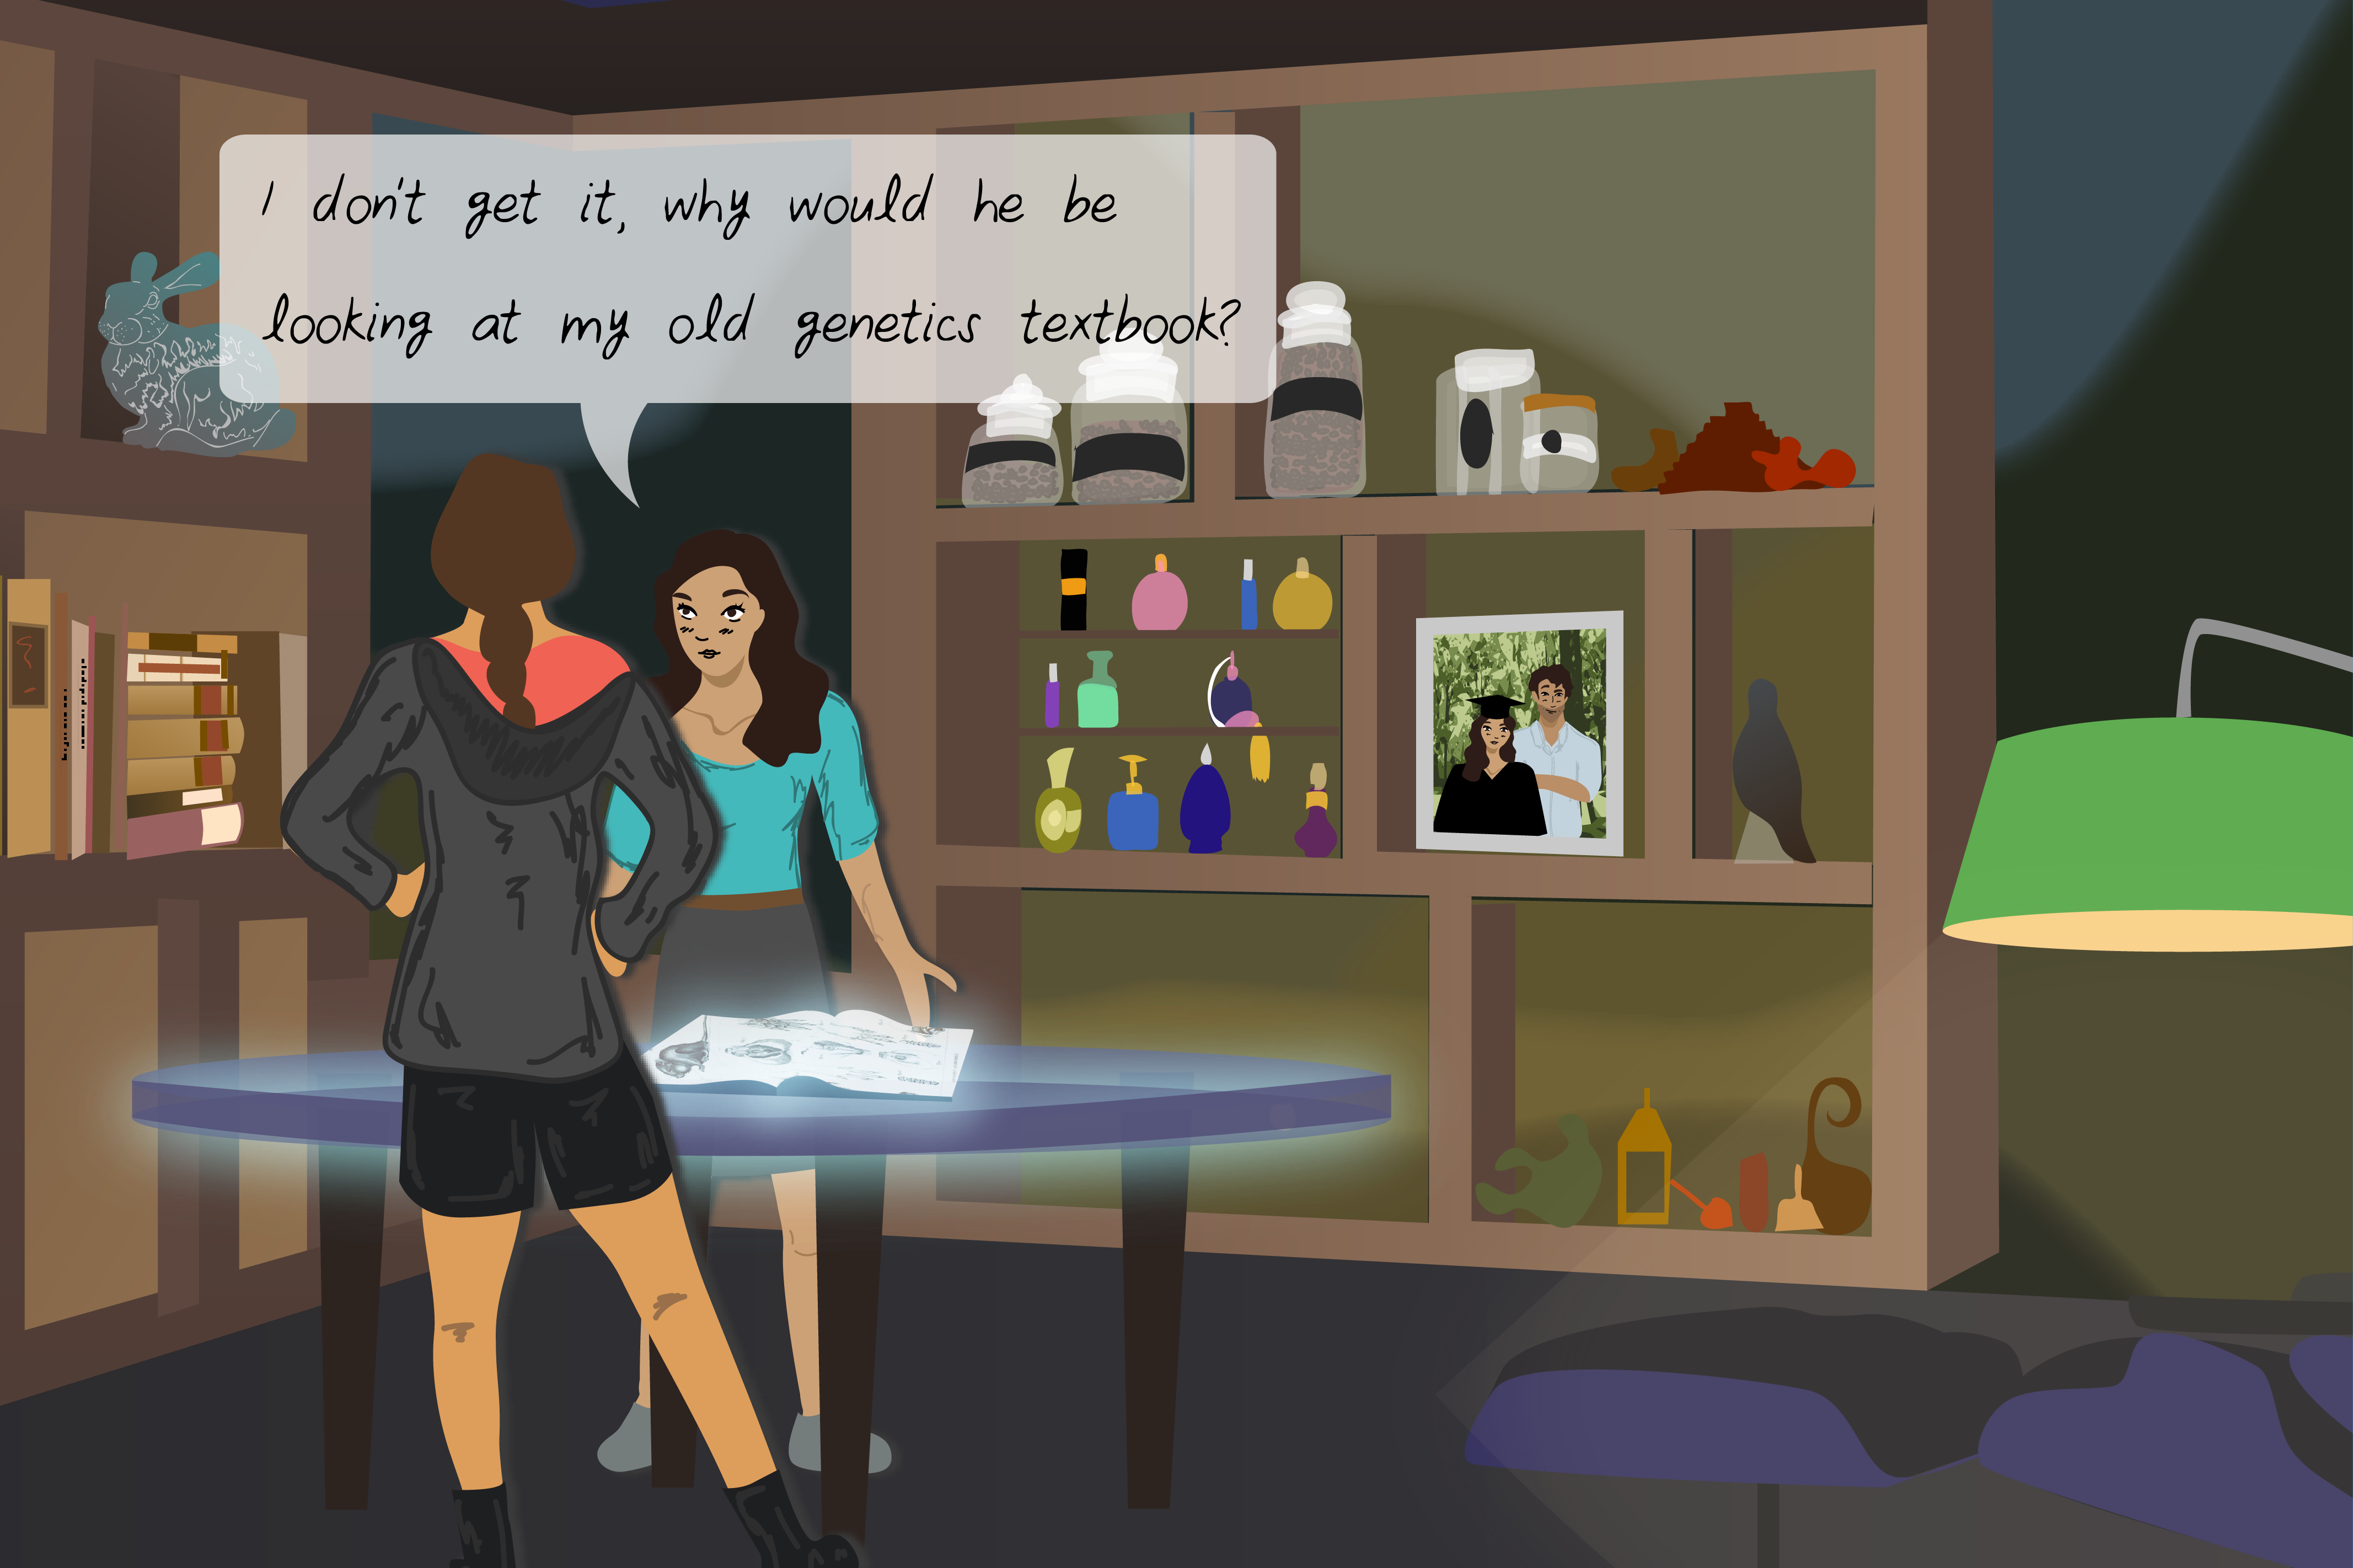
\includegraphics[width=2.5in]{figures/exp1/test-15.png} &
% 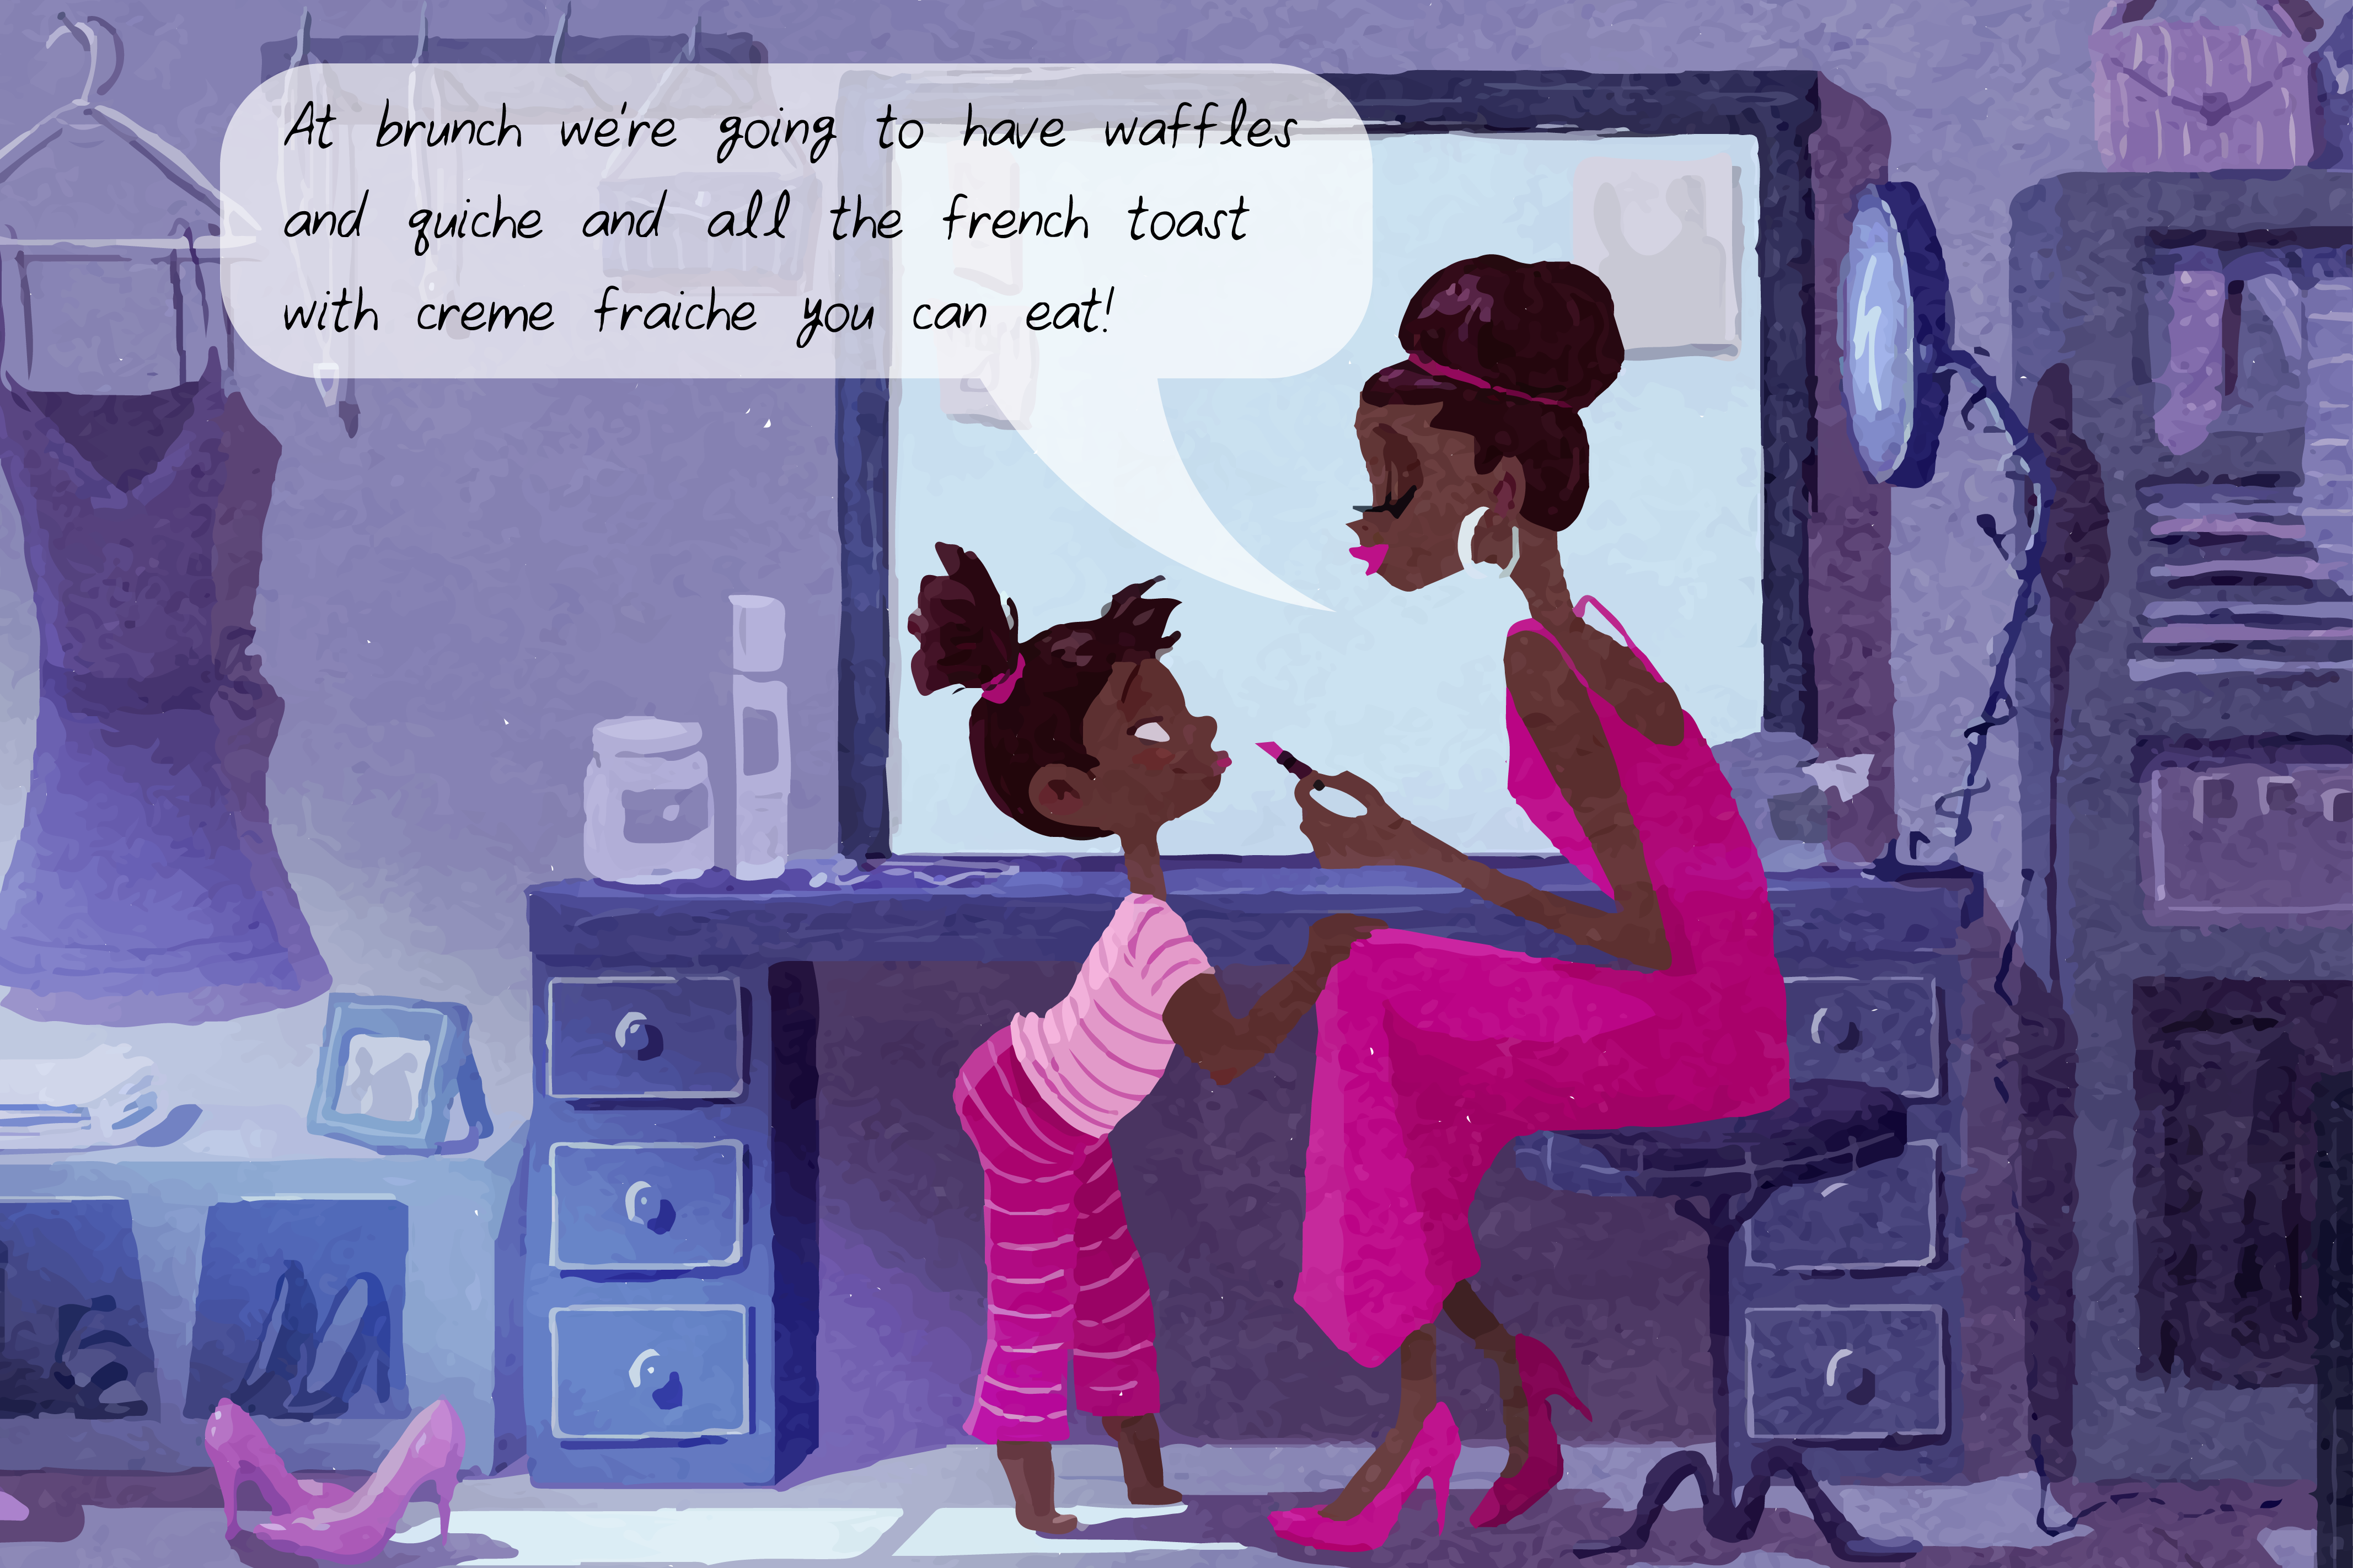
\includegraphics[width=2.5in]{figures/exp1/test-16.png} \\ 
% 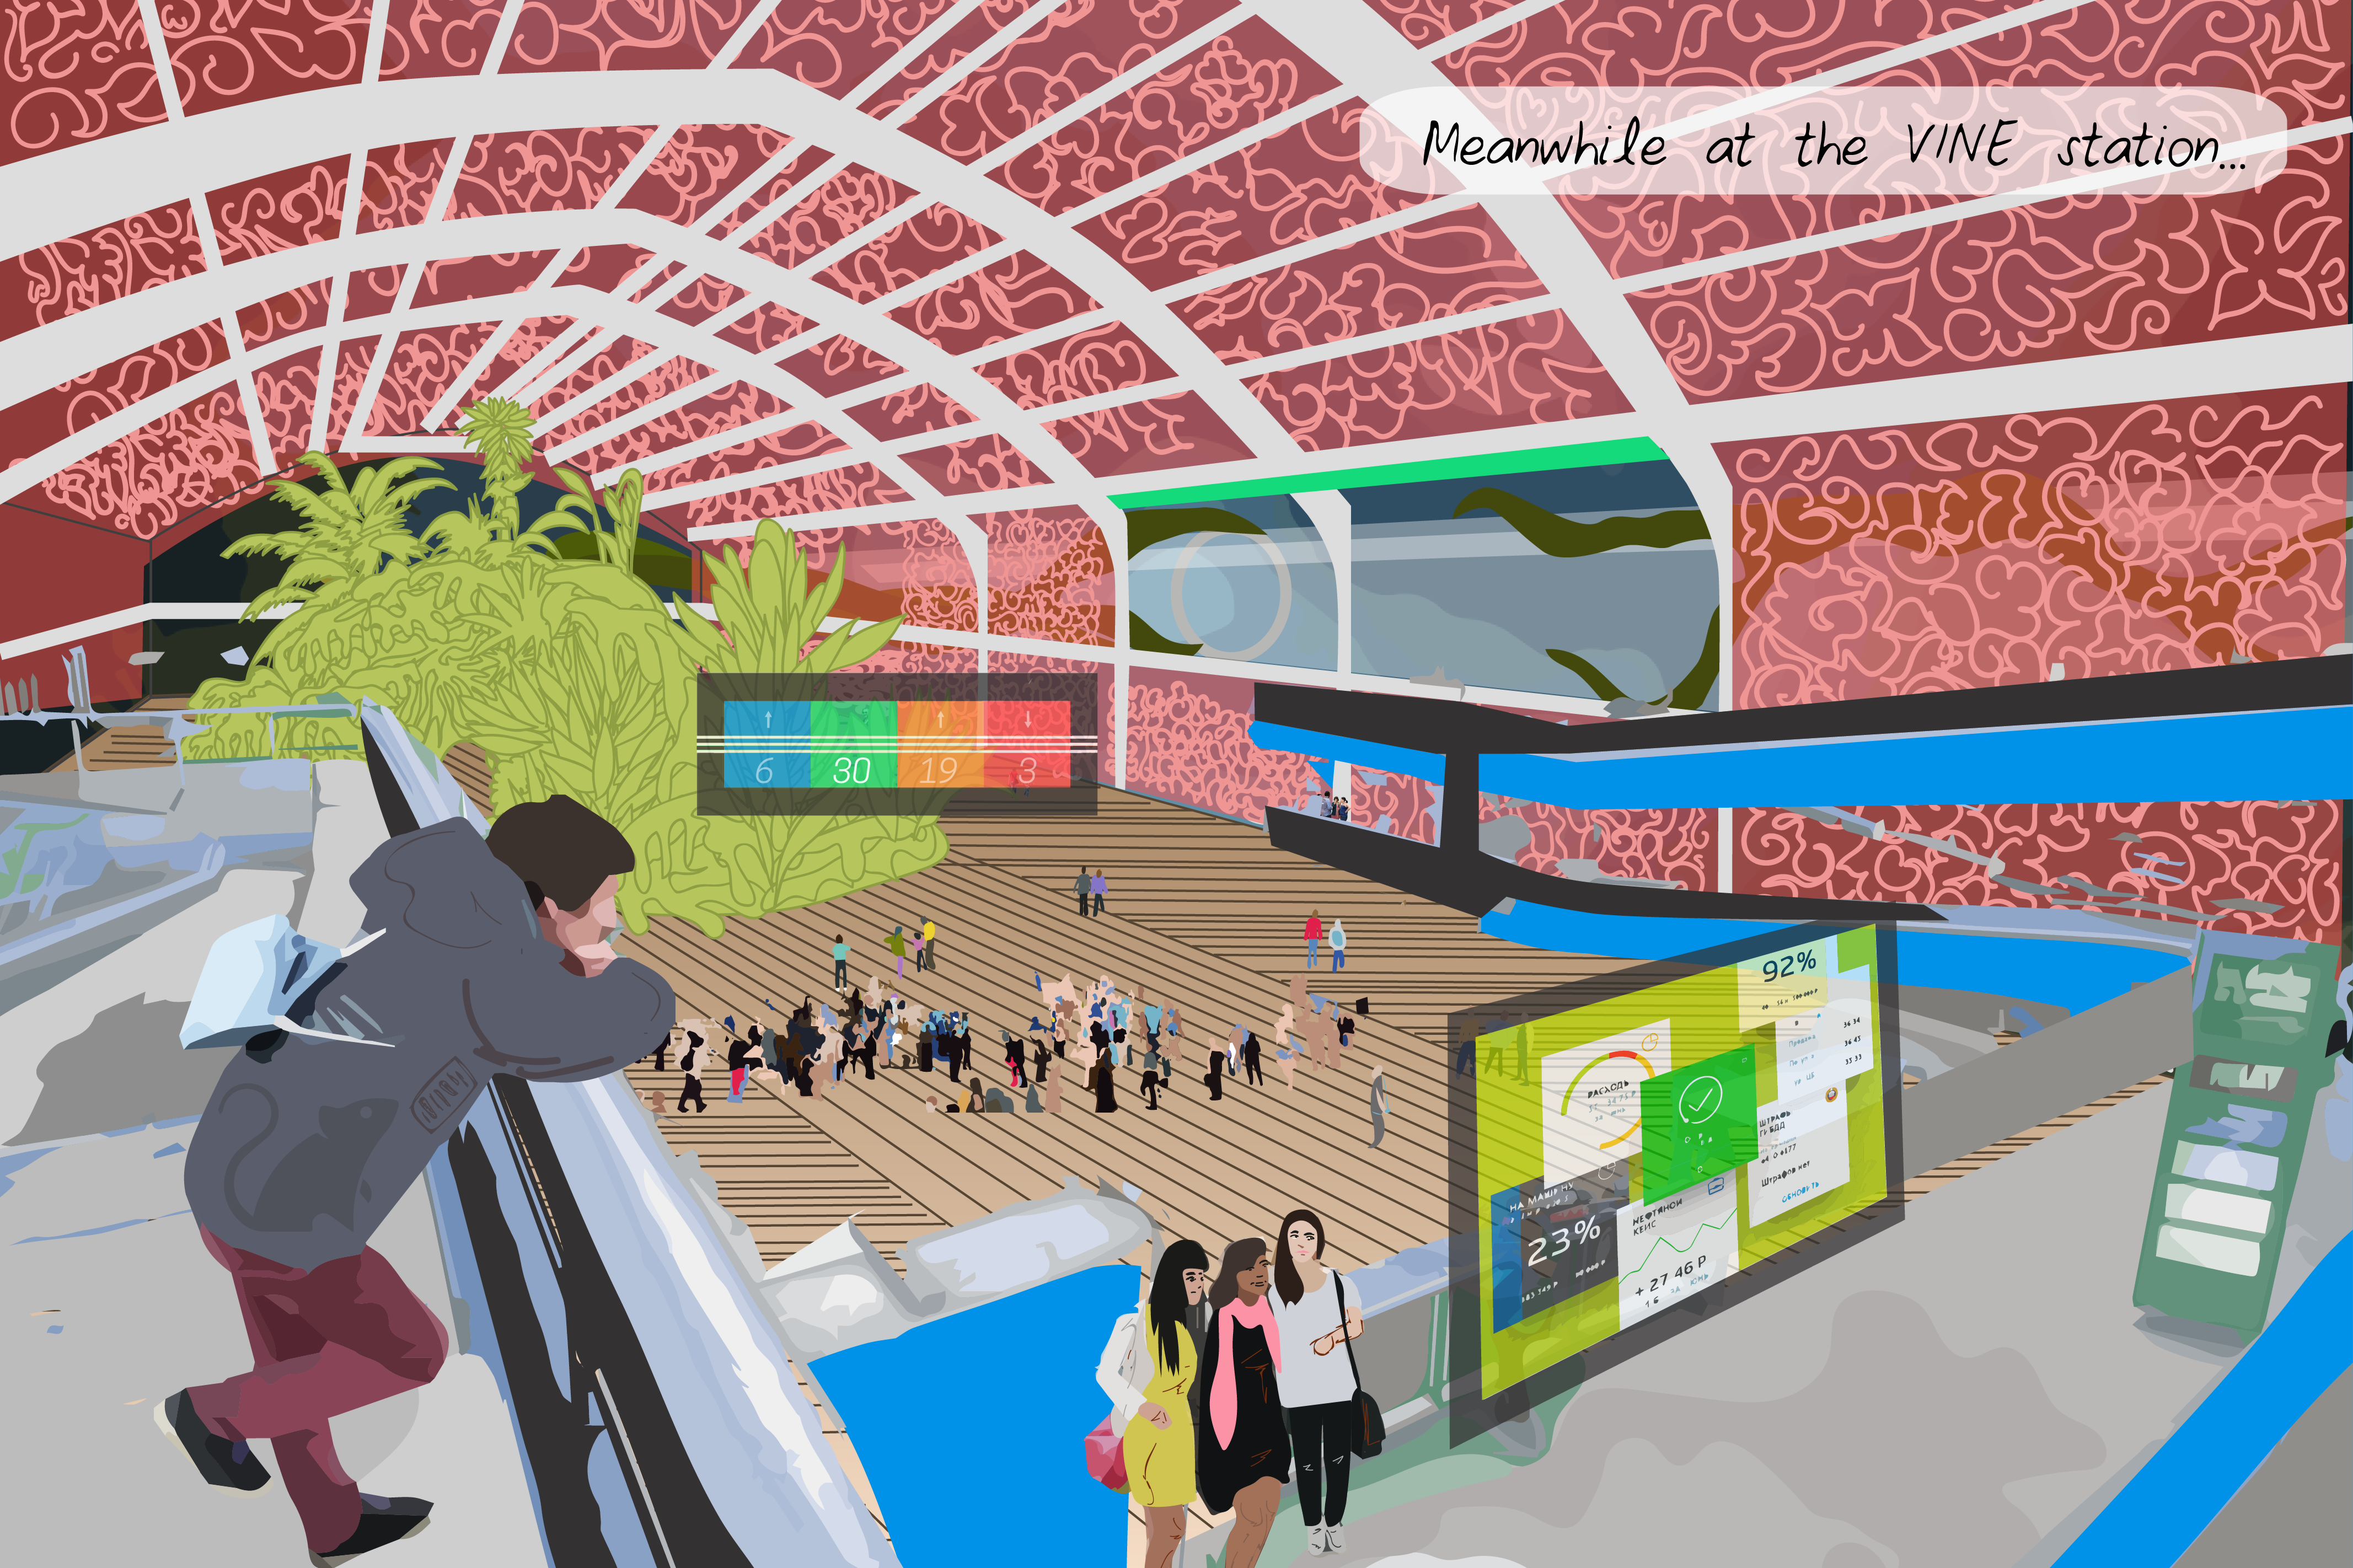
\includegraphics[width=2.5in]{figures/exp1/test-17.png} &
% \includegraphics[width=2.5in]{figures/exp1/test-18.png} \\ 
% 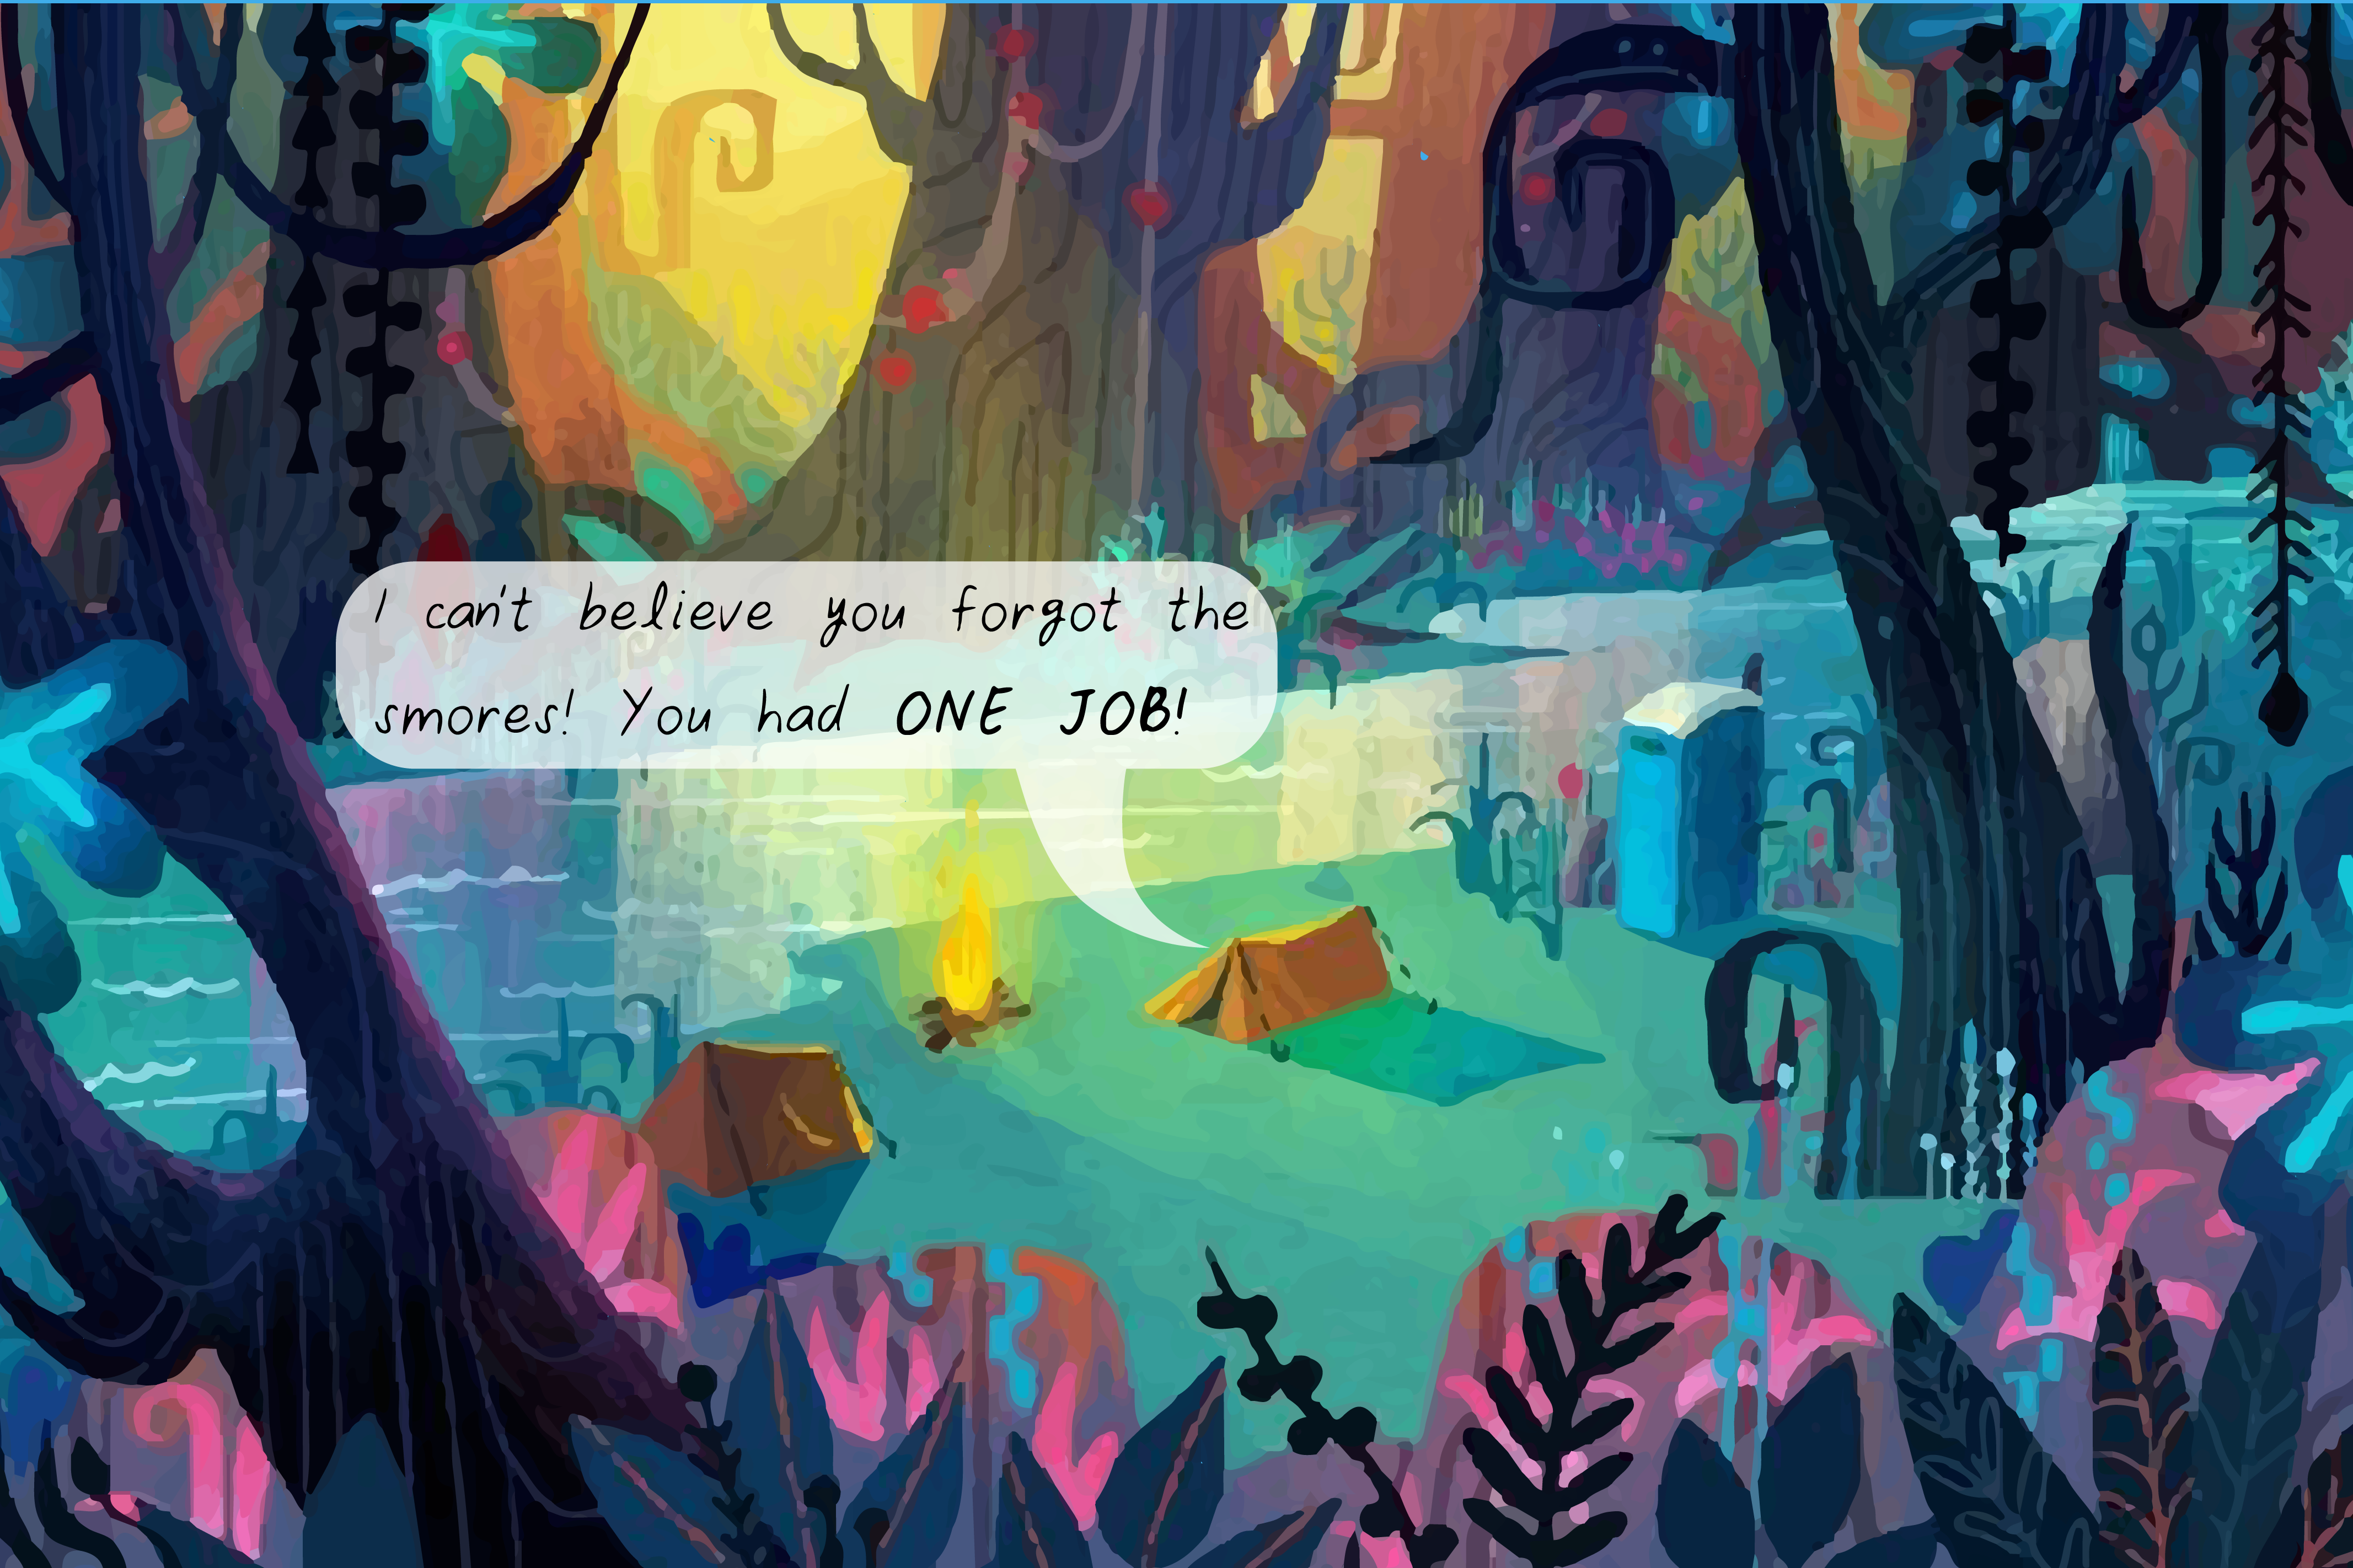
\includegraphics[width=2.5in]{figures/exp1/test-19.png} &
% 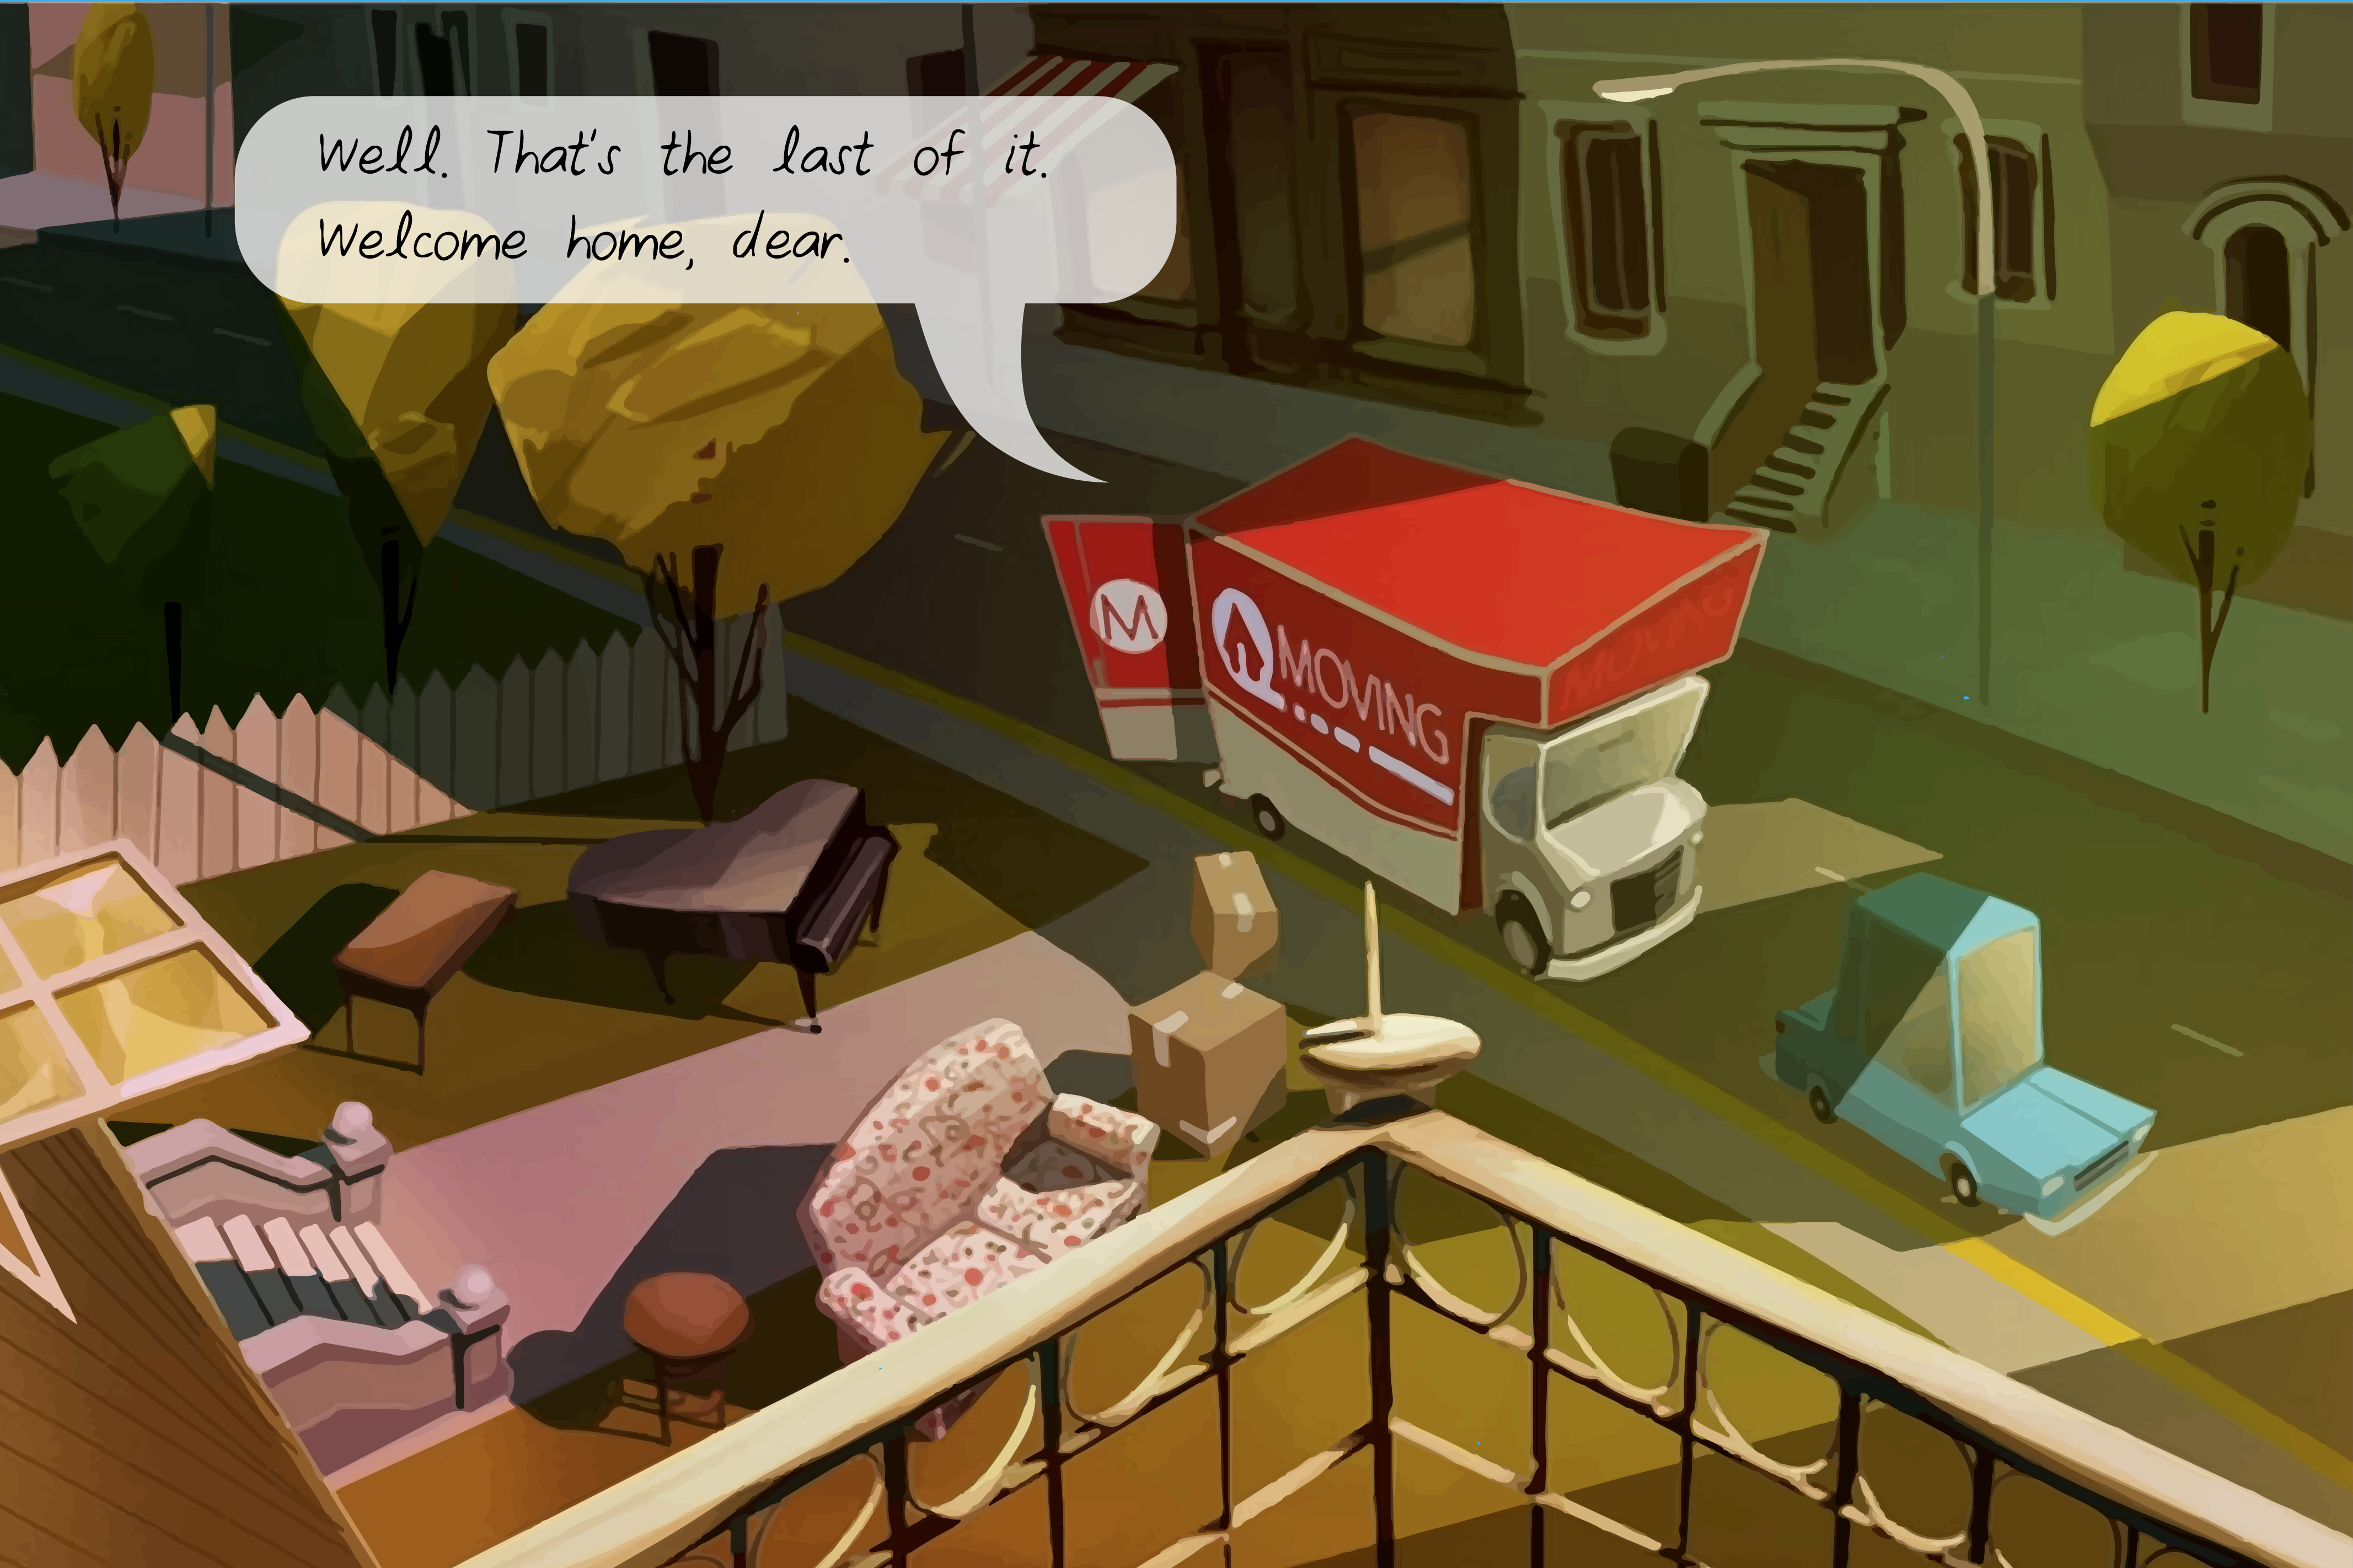
\includegraphics[width=2.5in]{figures/exp1/test-20.png}
% \end{array}$
% \end{center}
% \caption{Trial images from User Study 2, ctd.}
% \end{figure}
% 


\section*{Appendix B: User Study 2}
\addcontentsline{toc}{section}{Appendix B: User Study 2}

% Confidence interval:
%   The mean of	none minus greens equals -0.418776725758
%   95% confidence interval of this difference: From -0.822466706937 to -0.015086744578 
% Intermediate values used in calculations:
%   t = 2.2602
%   df = 12

% \begin{table}[h!]
% \centering
%  \begin{tabular}{|m{5em} || m{6em} | m{10em} | m{10em}|} 
%  \hline
%  Group & Affect & Adjectives & Next Day Plans \\ 
%  \hline\hline
%  none & 0.0516810976 & "boodle boodle" & "poodle doodles" \\ 
%  none & 0.636986 & "devious" & "chomp will eat the other fish" \\
%  greens & 0.8030303 & "adorable, heartwarming, calming, Nemo-like, colorful, whimsical" & "ill be another shark stereotype misunderstanding that is also resolved" \\
%  greens & 0.720838249 & "Active, Outgoing, Determined" & "He will make more friends" \\
%  greens & 0.7200083 & "nervous, eager, determined. lonely, friendly, motivated, unrelenting" & "ill have a picnic/lunch party (something where they all eat together)." \\
%  none & 0.74491477 & "timid, lonely, scared, shy, cautious, unsure" & "thing new and make even more friends. probubly go on an adventure " \\
%  none & 0.5 & "Friendly" & "he will make a new friend " \\
%  none & 0.0566625558 & "Naive, friendly, innocent, slow" & "They will have to hunt for food / eat things" \\
%  none & 0 & "Smiley, Nice, Hungry" & "Chomp's going to eat more fish." \\
%  greens & 0.9906599 & "sad, lonely, misunderstood, nice, friendly" & "Chomps will have a better day with his new sea friends" \\
%  none & 0.156289 & "Shy, ruthless, deceptive" & "Chomp will eat more of his classmates" \\
%  none & 0.5 & "Friendly" & "He struggles with his natural hunting instincts" \\
%  none & 0.114778049 & "accidental fish eater" & "i think he's going to eat more fish by accident" \\
%  none & 0.0525114536 & "crafty" & "Chomp will eat more of the "children"" \\
%  none & 0.807181537 & "Friendly, shy, and loyal" & "more friends and enjoy Ms Pufferfish's lesson plan, no matter what it is. \\ [1ex] 
%  \hline
%  \end{tabular}
% \end{table}


% \begin{figure}[h]
% \begin{center}$
% \begin{array}{c c}
% \includegraphics[width=2.5in]{figures/exp2_screencaps/01.png} &
% \includegraphics[width=2.5in]{figures/exp2_screencaps/02.png} \\ 
% \includegraphics[width=2.5in]{figures/exp2_screencaps/03.png} &
% \includegraphics[width=2.5in]{figures/exp2_screencaps/04.png} \\ 
% \includegraphics[width=2.5in]{figures/exp2_screencaps/05.png} &
% \includegraphics[width=2.5in]{figures/exp2_screencaps/06.png} \\ 
% \includegraphics[width=2.5in]{figures/exp2_screencaps/07.png} &
% \includegraphics[width=2.5in]{figures/exp2_screencaps/08.png} \\ 
% \includegraphics[width=2.5in]{figures/exp2_screencaps/09.png} &
% \includegraphics[width=2.5in]{figures/exp2_screencaps/10.png}
% \end{array}$
% \end{center}
% \caption{Trial images from User Study 2}
% \end{figure}

% \begin{figure}[h]
% \begin{center}$
% \begin{array}{c c}
% 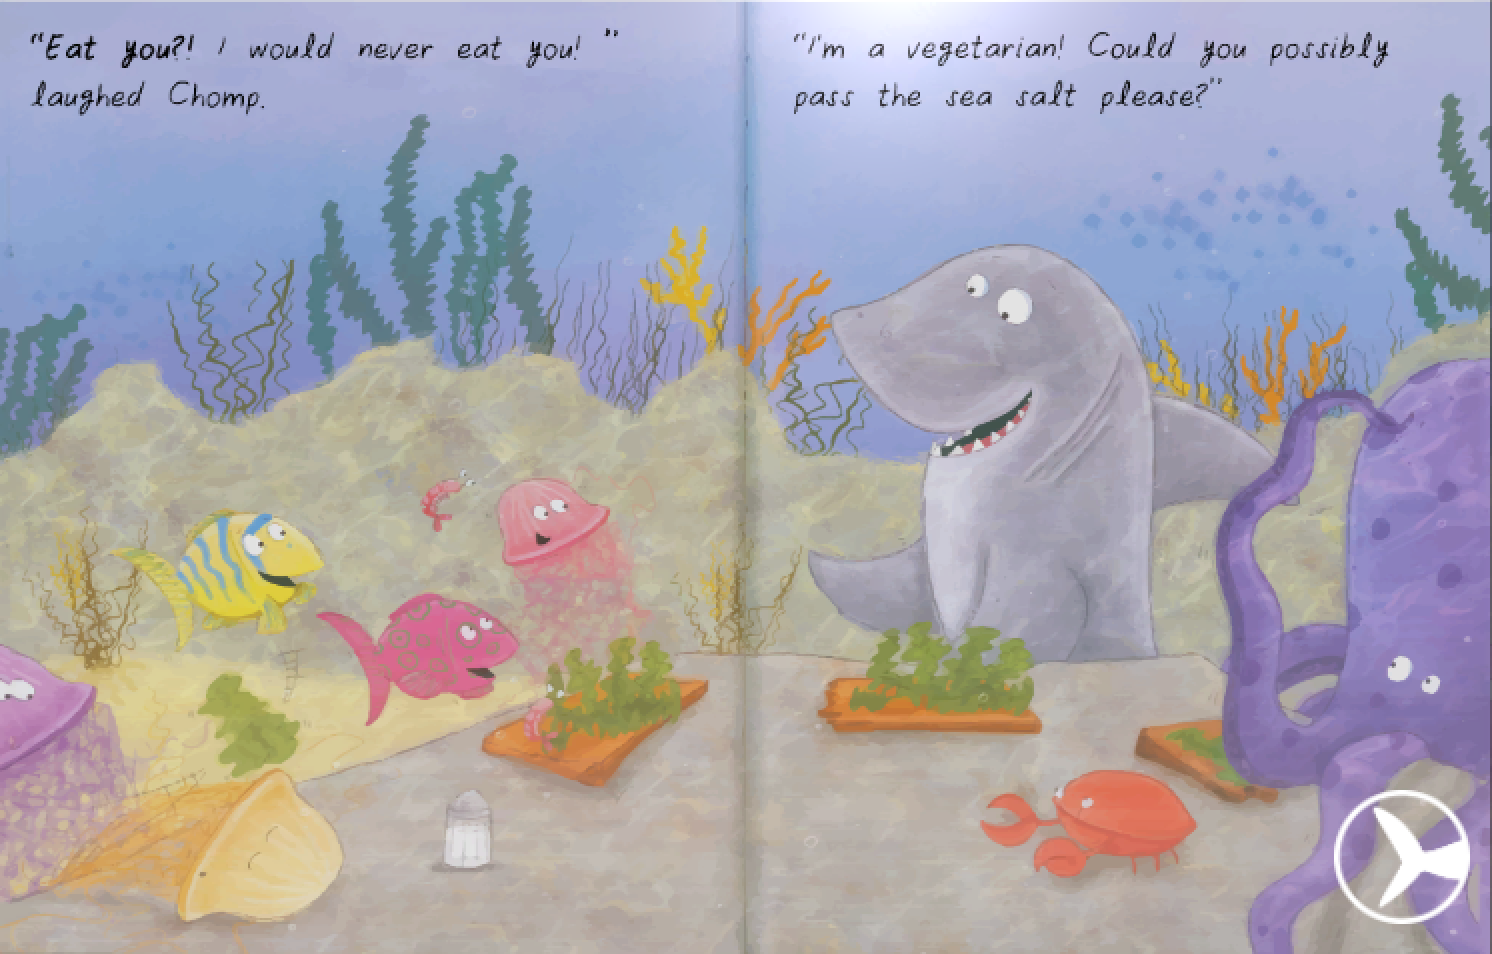
\includegraphics[width=2.5in]{figures/exp2_screencaps/11.png} &
% 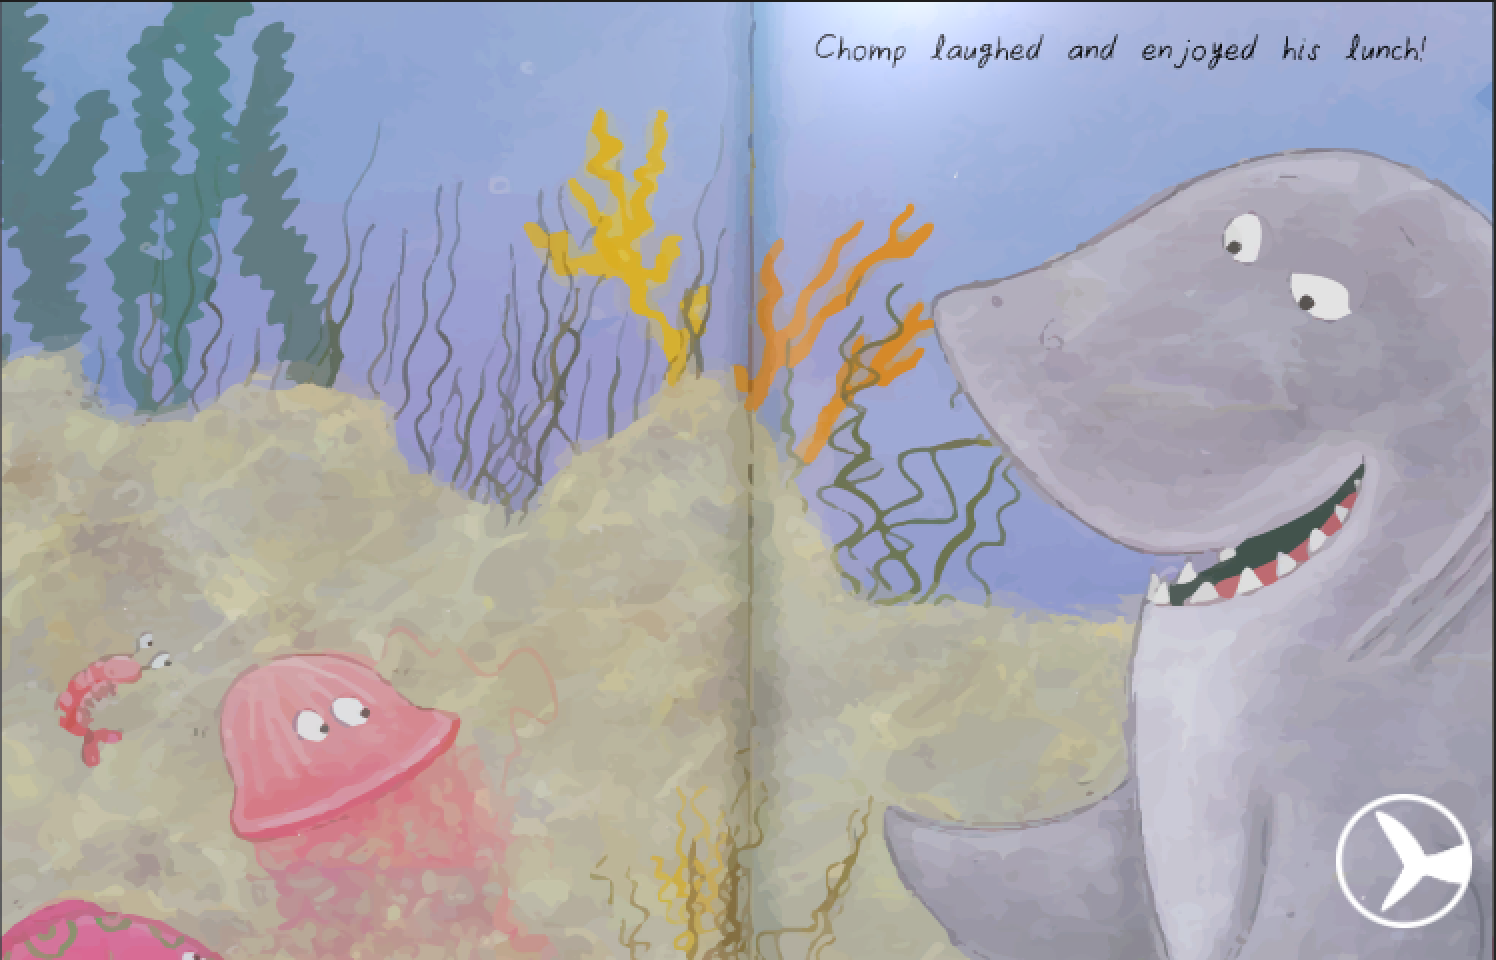
\includegraphics[width=2.5in]{figures/exp2_screencaps/11_alt.png} \\ 
% 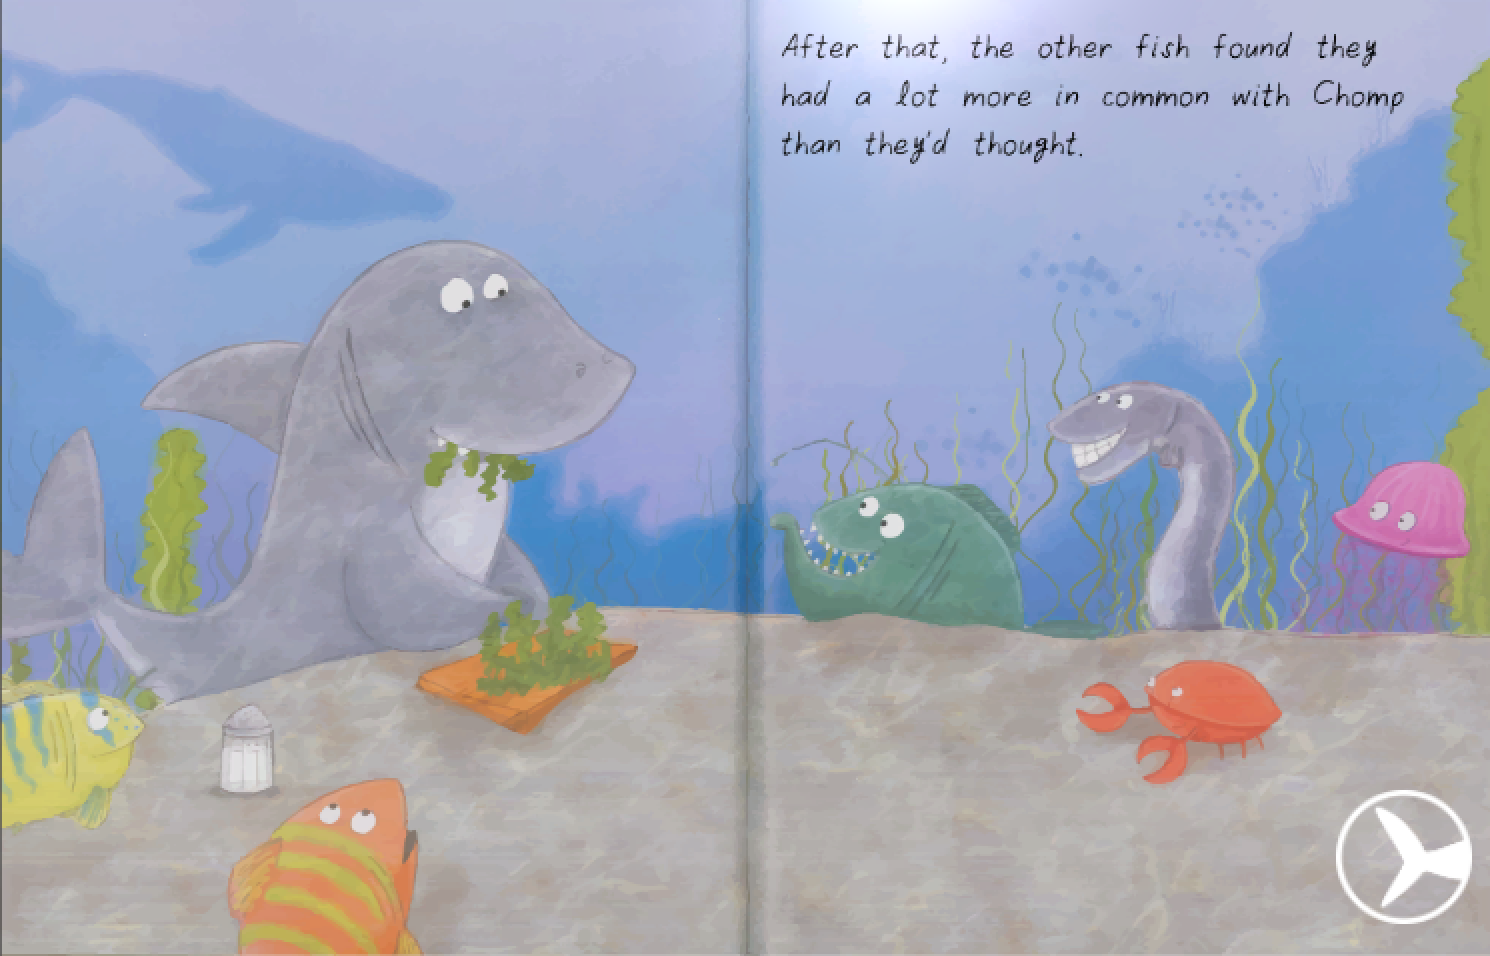
\includegraphics[width=2.5in]{figures/exp2_screencaps/12.png} &
% 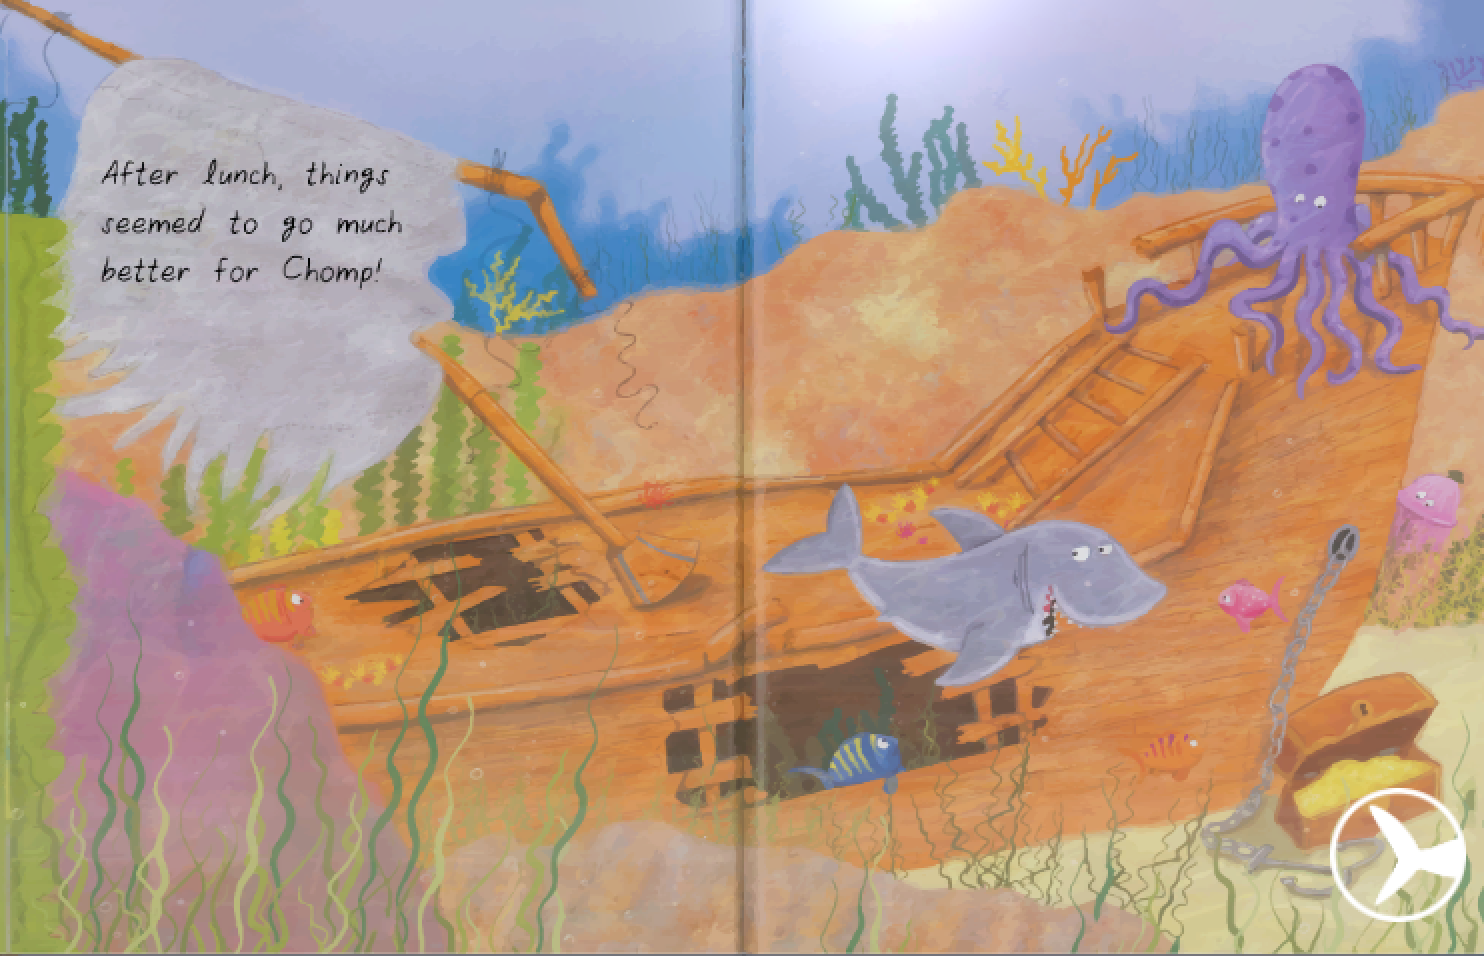
\includegraphics[width=2.5in]{figures/exp2_screencaps/13.png} \\ 
% 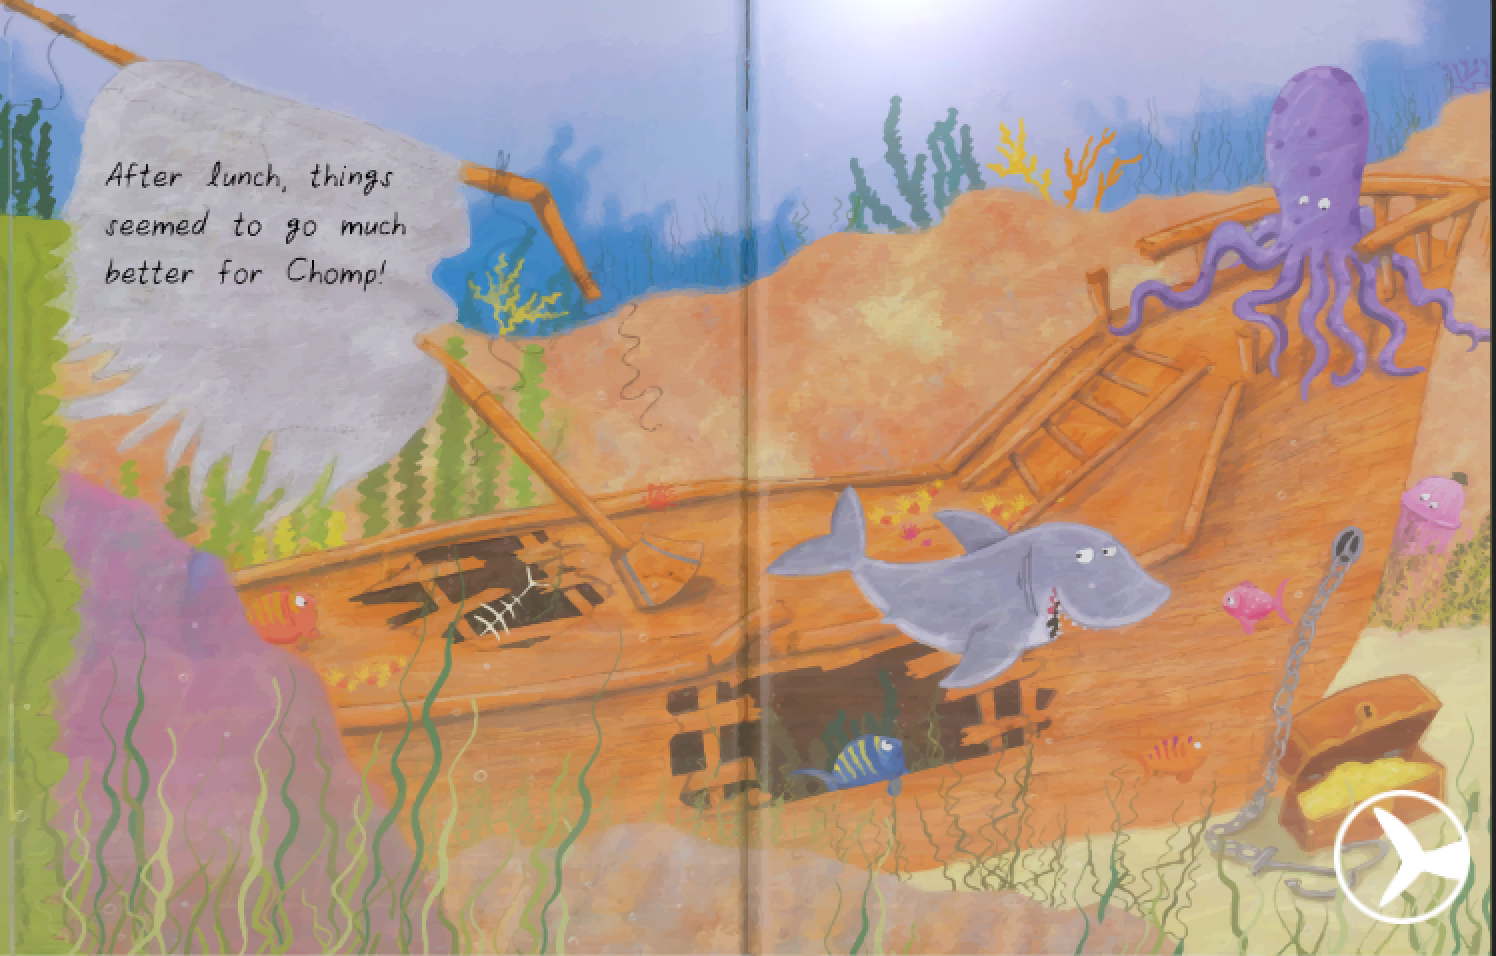
\includegraphics[width=2.5in]{figures/exp2_screencaps/13_alt.png} &
% 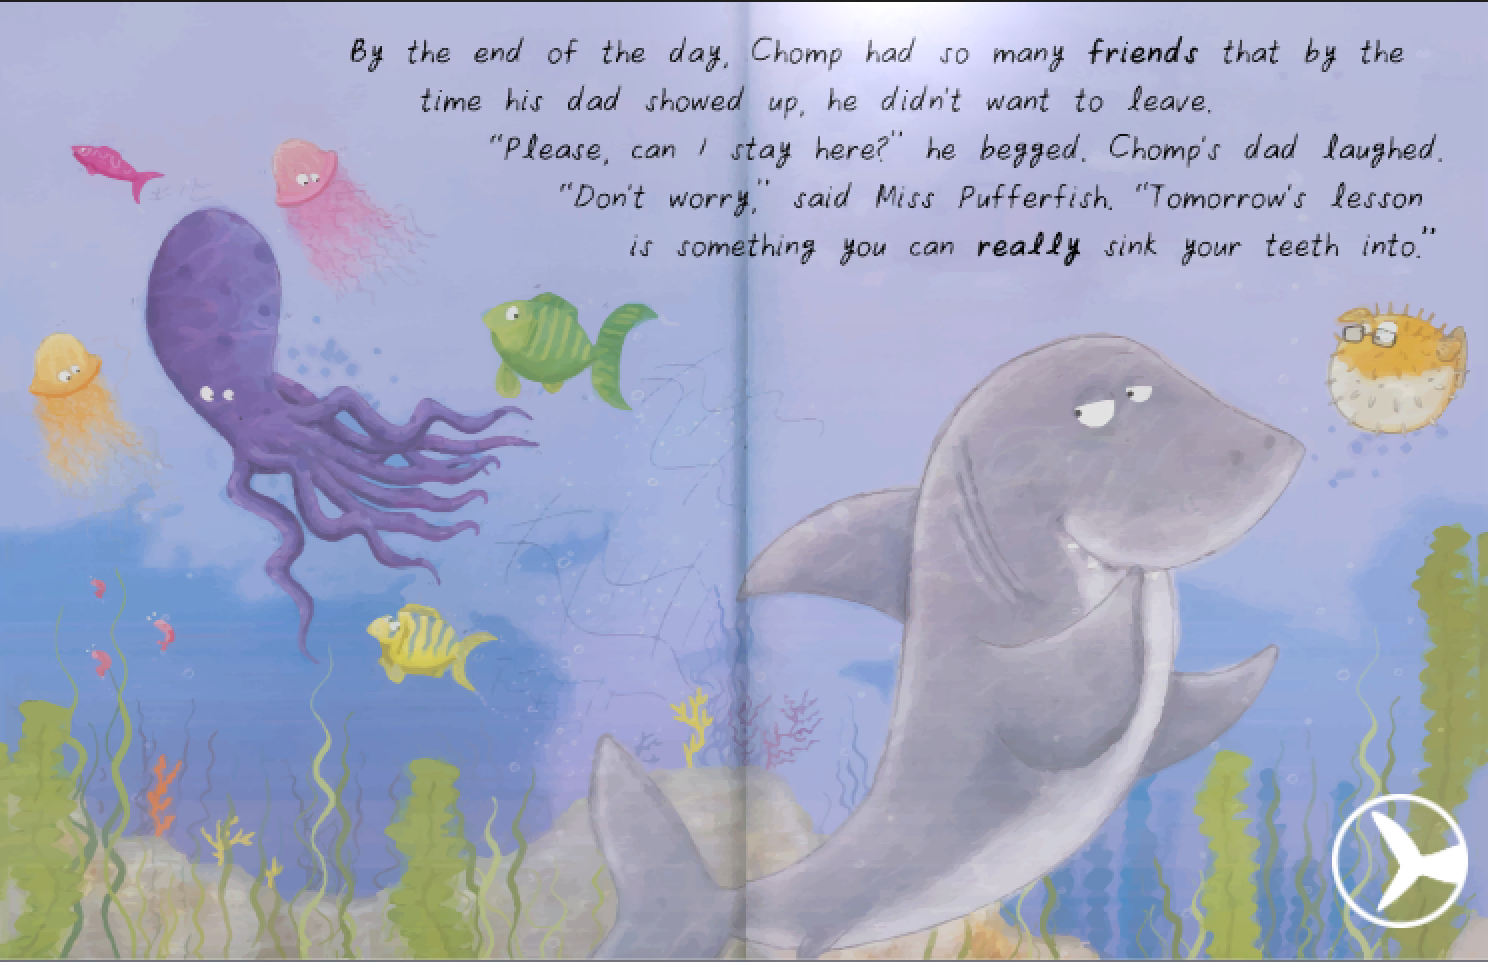
\includegraphics[width=2.5in]{figures/exp2_screencaps/14.png} \\ 
% 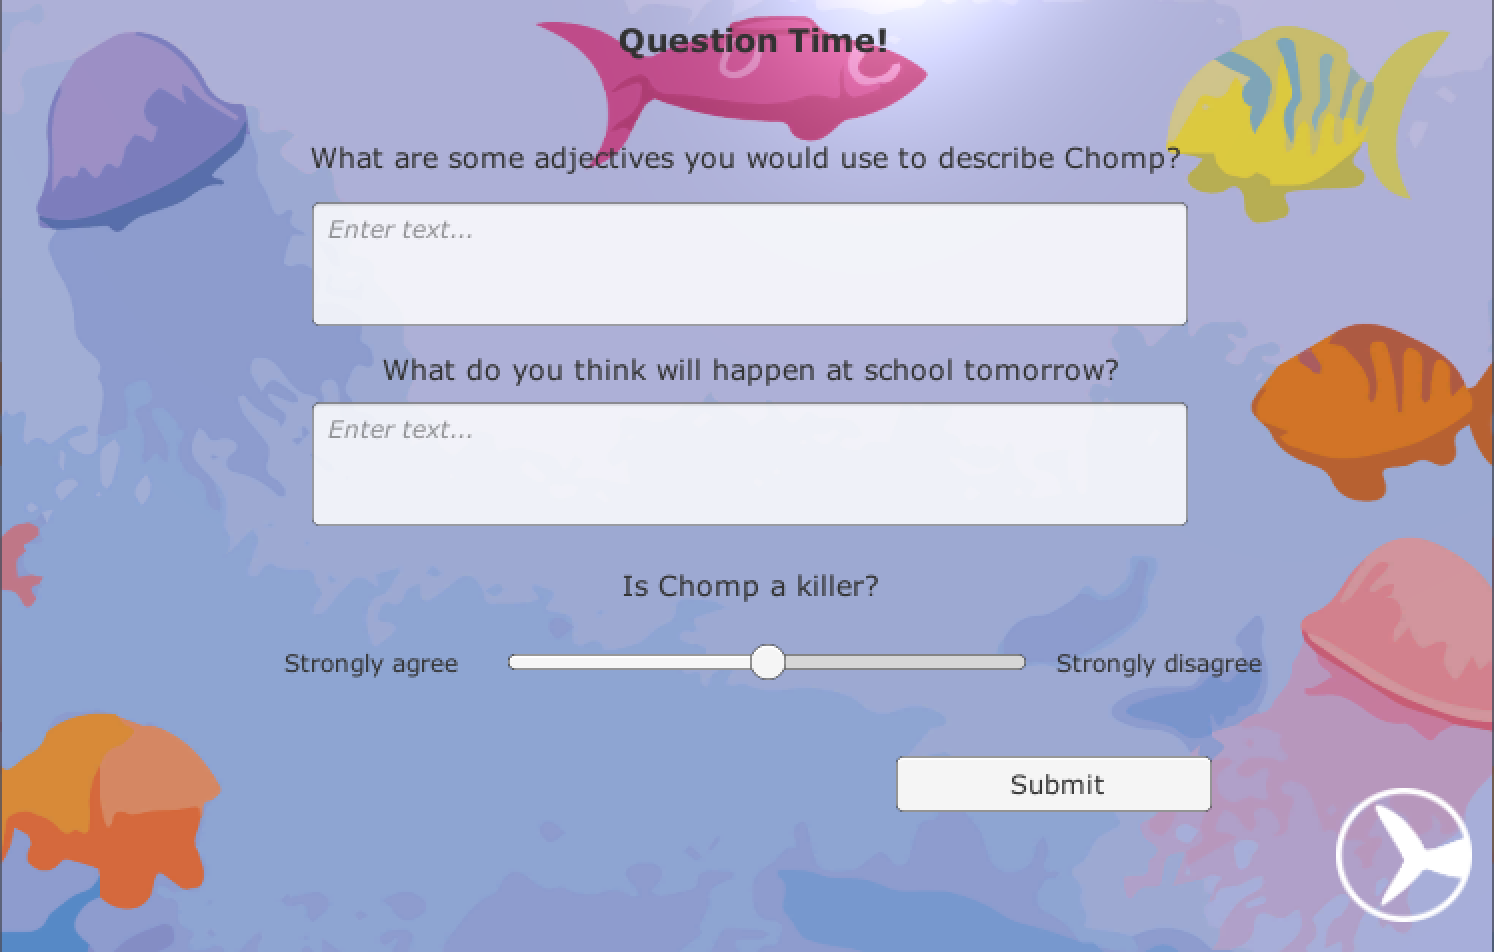
\includegraphics[width=2.5in]{figures/exp2_screencaps/15.png} &
% 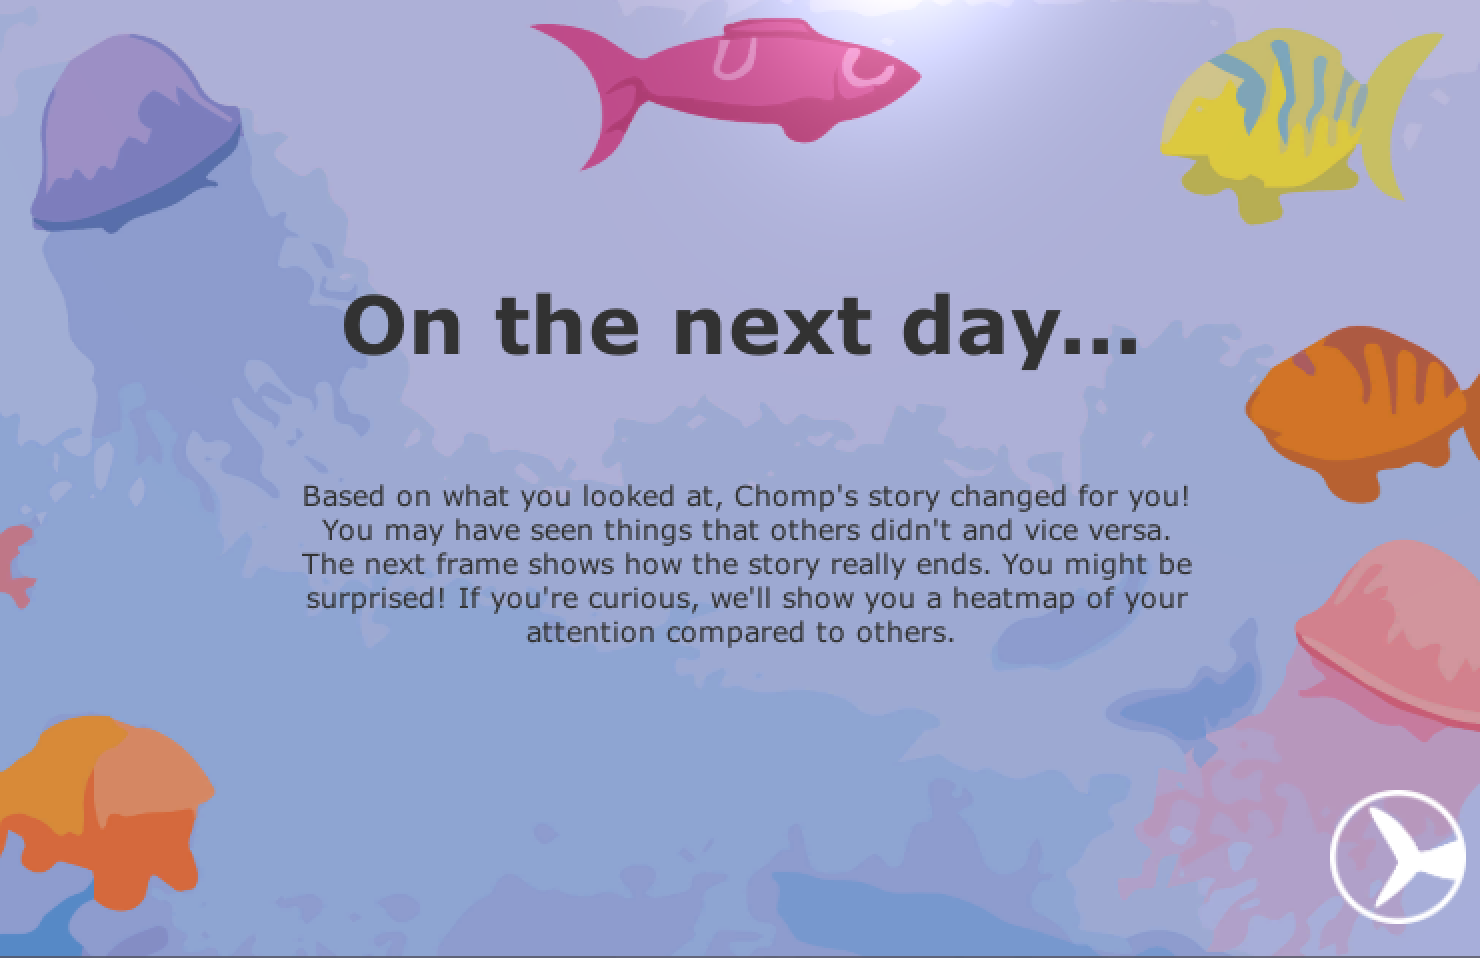
\includegraphics[width=2.5in]{figures/exp2_screencaps/16.png} \\ 
% 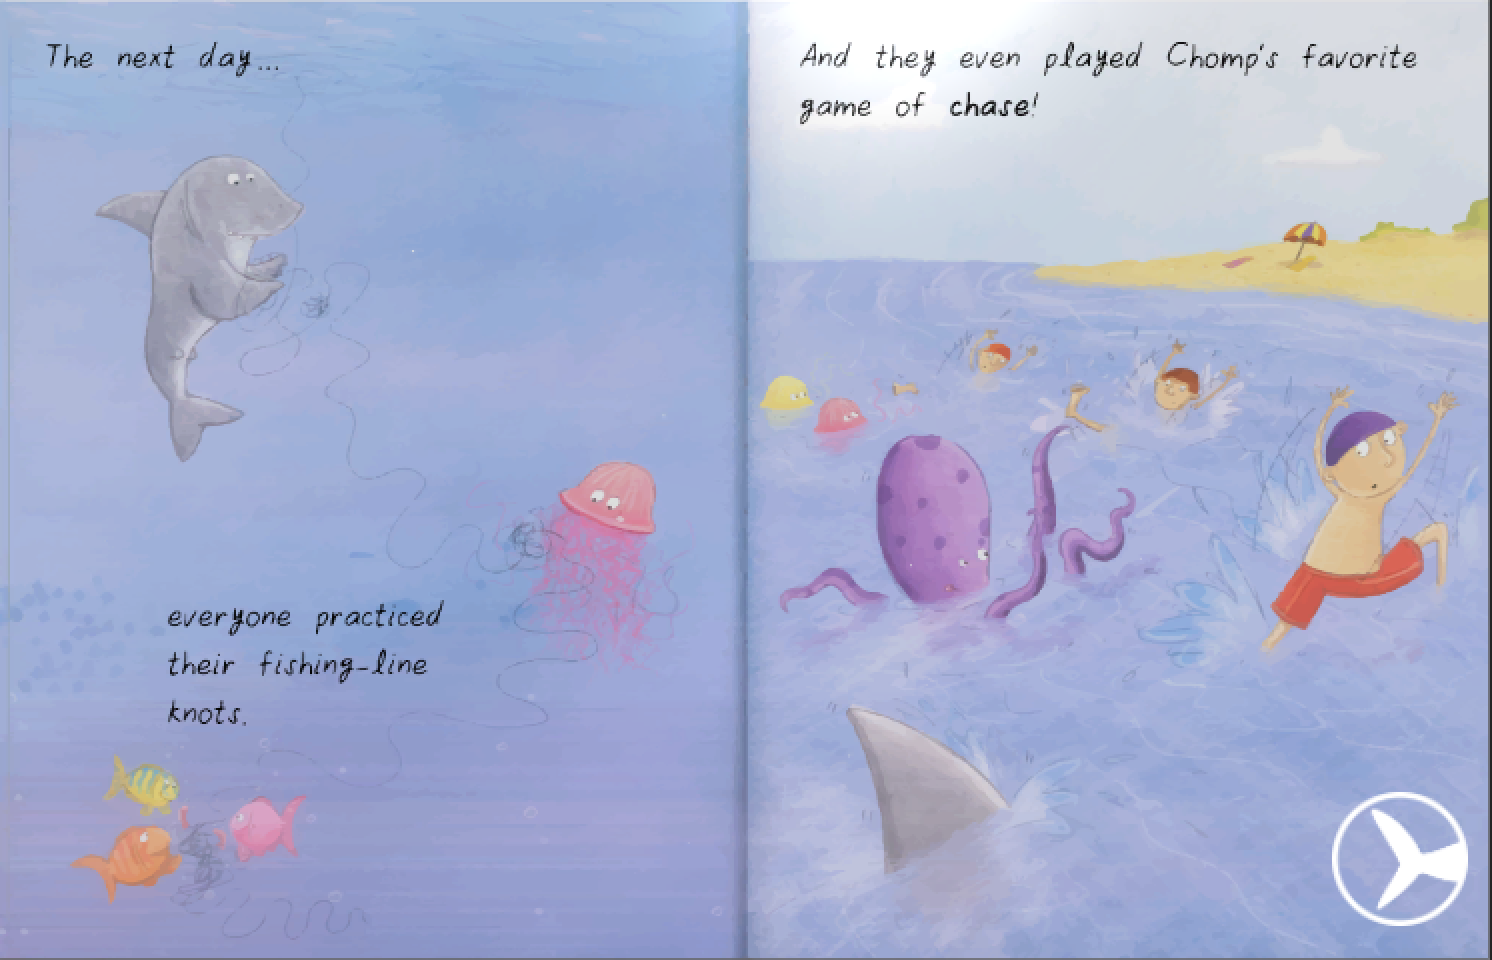
\includegraphics[width=2.5in]{figures/exp2_screencaps/17.png} &
% 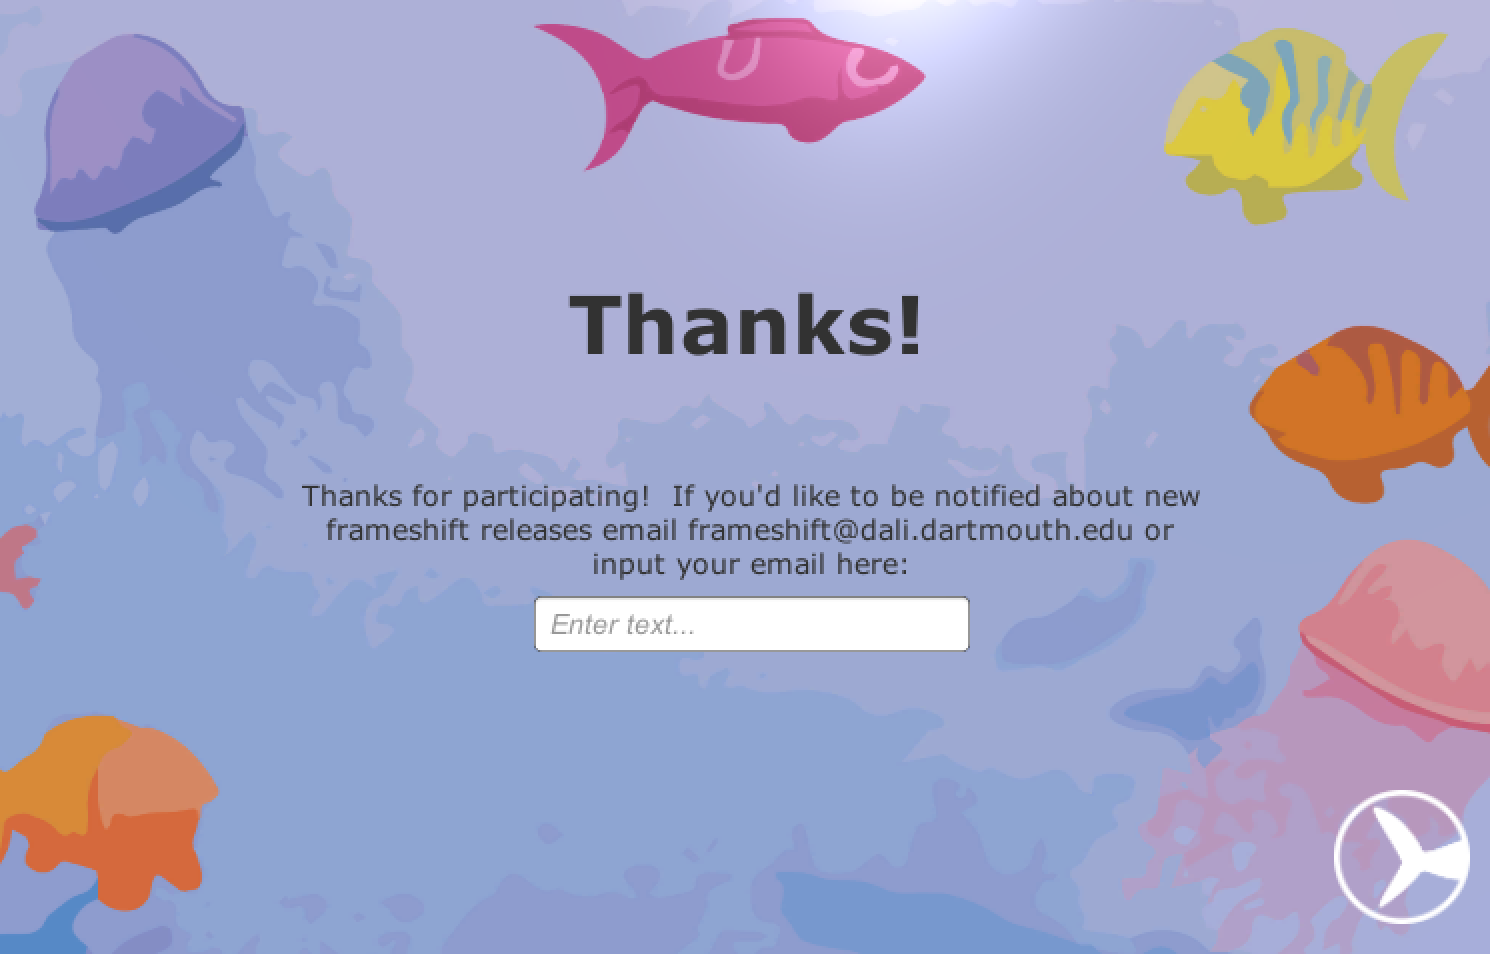
\includegraphics[width=2.5in]{figures/exp2_screencaps/18.png}
% \end{array}$
% \end{center}
% \caption{Trial images from User Study 2, ctd.}
% \end{figure}






% 

\section*{Appendix C: Distribution of Work}
\addcontentsline{toc}{section}{Appendix C: Distribution of Work}

% As part of the requirement for a joint thesis this sections identifies the different work performed by each of the two authors. 

% Rukmini Goswami took the lead on:
% \begin{itemize}
%  \setlength\itemsep{-0.5em}
%  \item user study design and process
%  \item analysis of results
%  \item experimental setup in Unity3D
%  \item EyeTribe initial experimentation
%  \item statistical methods
%  \item all artwork for the future work
% \end{itemize}

% Tim Tregubov took the lead on: 
% \begin{itemize}
%  \setlength\itemsep{-0.5em}
%  \item scaffolding out the Unity3D C\# classes and framework. 
%  \item designing the narrative framework structure
%  \item Tobii SDK integration
%  \item gaze and fixation data processing
%  \item stack architecture and code structure
% %  \begin{itemize}
% %     \setlength\itemsep{-0.5em}
% %     \item for thi
% %  \end{itemize}
% \end{itemize}

 
% \section*{Appendix D: Preview images from FrameShift the novel}
\addcontentsline{toc}{section}{Appendix D: Preview images from FrameShift — the novel}
% \begin{figure}[h!]
% \begin{center}$
% \begin{array}{c c}
% \includegraphics[width=2.3in]{figures/appendixD/01.png} &
% \includegraphics[width=2.3in]{figures/appendixD/02.png} \\ 
% \includegraphics[width=2.3in]{figures/appendixD/03.png} &
% \includegraphics[width=2.3in]{figures/appendixD/04.png} \\ 
% \includegraphics[width=2.3in]{figures/appendixD/05.png} &
% \includegraphics[width=2.3in]{figures/appendixD/06.png} \\ 
% \includegraphics[width=2.3in]{figures/appendixD/07.png} &
% \includegraphics[width=2.3in]{figures/appendixD/08.png} \\ 
% \includegraphics[width=2.3in]{figures/appendixD/09.png} &
% \includegraphics[width=2.3in]{figures/appendixD/10.png}
% \end{array}$
% \end{center}
% \end{figure}

\singlespacing

\bibliography{nook_citations}
\addcontentsline{toc}{chapter}{Bibliography}



\end{document}
